\documentclass[a4paper,12pt]{report}
\usepackage[T1]{fontenc}
\usepackage[utf8]{inputenc}
\usepackage[italian,english]{babel}
% LAYOUT
\usepackage{geometry}
	\geometry{a4paper,top=2.8cm,headsep=1.2cm,bottom=2.5cm,
	left=2.5cm,right=2.5cm,heightrounded}
\usepackage[titletoc]{appendix}
\usepackage[autostyle,italian=guillemets,english=american]{csquotes}
\usepackage[backend=biber,style=numeric,hyperref]{biblatex}
	\addbibresource{bibliography.bib}
\usepackage{hyperref}
	\hypersetup{hidelinks}
\usepackage{microtype}
% SCIENTIFIC TYPESETTING
\usepackage{amsmath, amsthm, amssymb, mathtools}
\usepackage{siunitx}
\usepackage{resizegather}
	\addtolength{\jot}{4pt}
\usepackage{bm, mathrsfs}
% FIGURES AND TABLES
\usepackage{pgfplots, pgfplotstable, booktabs, array}
	\pgfplotsset{compat=1.16}
	\pgfplotstableset{
		col sep = comma,
		every head row/.append style={before row=\toprule, after row=\midrule},
		every last row/.append style={after row=\bottomrule},
		every column/.append style={sci, sci zerofill, sci e, sci precision = 2},
		string replace={NaN}{},
		empty cells with={-}
	}
\usepackage{listingsutf8}
	\lstset{inputencoding=utf8/latin1}
	\lstset{numbers=left, frame=tb, rulecolor=\color{black}}
	\lstset{framexleftmargin=3em, xleftmargin=3em}
	\lstset{tabsize=4}
	\lstset{captionpos=b, abovecaptionskip=1ex}
	\renewcommand{\lstlistingname}{Program}
\usepackage{matlab-prettifier}
	\lstset{style=Matlab-editor}
\usepackage[scaled]{beramono}
	\lstset{basicstyle=\mlttfamily \small}
	\lstset{numberstyle=\mlttfamily \small \color{gray}}
\usepackage{caption, subcaption}
	\captionsetup{tableposition=top,figureposition=bottom}
	\captionsetup{justification=centering,font=small,labelfont=bf}


\renewcommand{\vec}[1]{\bm{#1}}
\newcommand{\mat}[1]{\bm{#1}}
\newcommand{\tns}[1]{\bm{#1}}

\newcommand{\N}{\mathbb{N}}
\newcommand{\Z}{\mathbb{Z}}
\newcommand{\Q}{\mathbb{Q}}
\newcommand{\R}{\mathbb{R}}
\newcommand{\C}{\mathbb{C}}
\newcommand{\abs}[1]{\left\lvert#1\right\rvert}
\newcommand{\norm}[1]{\left\lVert#1\right\rVert}
\newcommand{\deq}{\vcentcolon=}
\newcommand{\eqd}{=\vcentcolon}
\newcommand{\dx}{\, d\vec{x}}
\newcommand{\dt}{\, dt}
\newcommand{\dsigma}{\, d\vec{\sigma}}
\newcommand{\grad}{\nabla}
\renewcommand{\Re}{\operatorname{Re}}
\renewcommand{\Im}{\operatorname{Im}}

\DeclareMathOperator{\Ker}{Ker}
\DeclareMathOperator{\Rank}{Rank}
\DeclareMathOperator{\spn}{span} % \span è già utilizzato da latex
\DeclareMathOperator{\diver}{div}
\DeclareMathOperator{\supp}{supp}
\DeclareMathOperator{\TV}{TV}
\DeclareMathOperator{\tr}{tr}

\theoremstyle{definition}
\newtheorem*{defi}{Definition}
\newtheorem*{exam}{Example}
\newtheorem*{prob}{Problem}

\theoremstyle{plain}
\newtheorem{theo}{Theorem}[chapter]
\newtheorem{lemm}[theo]{Lemma}
\newtheorem{prop}[theo]{Proposition}
\newtheorem{coro}[theo]{Corollary}

\theoremstyle{remark}
\newtheorem*{rema}{Remark}

\begin{document}

\begin{titlepage}
\newgeometry{top=2cm,bottom=2cm,left=3cm,right=3cm,heightrounded}
\begin{figure}[htbp]
\begin{minipage}{0.3\textwidth}

\includegraphics[scale=1.1]{figures/logo.pdf}
\end{minipage}
%
\hfill
%
\begin{minipage}{0.4\textwidth}
\centering
\begin{flushright}
	{\Large \textbf{Scuola di Scienze\\ Matematiche\\ Fisiche e Naturali\\}}
\end{flushright}
\begin{flushright}
	Corso di Laurea Magistrale\\ in Matematica
\end{flushright}
\end{minipage}
%
\end{figure}
\vspace{20mm}
\begin{center}
	{\Huge \textbf{Numerical solution of the 2D\\ compressible Euler equations\\
	using WENO reconstructions\\ on polygonal meshes\\}}
	\vspace{10mm}
	{\huge Soluzione numerica delle equazioni di\\ Eulero
	per fluidi comprimibili in due\\ dimensioni
	mediante ricostruzioni\\ WENO su mesh poligonali\\}
\end{center}
\vspace{25mm}
\noindent{\Large \textbf{Relatrice:}   \\ \\}
\noindent{\LARGE Prof.\ Alessandra Sestini \\ \\}
\noindent{\Large \textbf{Candidato:}  \\ \\}
\noindent{\LARGE Bruno Degli Esposti \\ \\}
\vfill
\noindent{\normalsize Anno accademico 2020/2021}

\end{titlepage}
\newpage
\restoregeometry

\tableofcontents
\pagestyle{headings}

\chapter*{Introduction} \label{ch:introduction}
%\phantomsection
\addcontentsline{toc}{chapter}{Introduction}

Fast, accurate and reliable simulations of transport phenomena are of great
importance to scientific and engineering applications, but to this day remain
challenging despite decades of effort in the field of numerical analysis.

The reasons are manifold: first, the interplay between the numerical domain
of dependence at every point and the analytical domain of dependence is very
delicate and, if not handled correctly, can easily lead to the definition
of unstable numerical methods.
%(hence the need for upwinding, CFL conditions, etc).

Second, weak diffusion terms in the equations (or the lack thereof) allow
sharp features of the solution to propagate without substantial smoothing
effects. This a problem for low order numerical schemes, which suffer from
excessive dissipation, but also for high order schemes, which rely on regularity
assumptions that may only hold piecewise on the exact solution.
Moreover, in the inviscid nonlinear case, even smooth initial boundary
data can develop discontinuities in finite time due to wave-breaking phenomena.

And finally, a convergent numerical scheme can still produce unsatisfactory results
from a qualitative point of view, because it may not enforce exact
conservation at the discrete level, or it may produce spurious oscillations
around sharp features, or it may even converge to the wrong kind of weak
solution (for example, one that violates a suitable generalization of the
second law of thermodynamics).

In this work, we tackle some of these issues in the context of the
numerical solution of the 2D compressible Euler equations,
which are among the most important examples of hyperbolic systems of
conservation laws both from a practical and a historical point of view.
Our approach builds on well-established but modern techniques that
combine the finite volume method (FVM) with Godunov’s method and Weighted
Essentially Non-Oscillatory (WENO) reconstructions based on least-squares
polynomial approximation, following the works of Hu and Shu and others
\cite{hu1999weighted} \cite{kaser2005ader}.

After an introduction to the 2D compressible Euler equations
and the finite volume method, we define numerical schemes
of arbitrarily high order for the solution of hyperbolic systems
of conservation laws by using a least-squares polynomial approximation
technique. The resulting schemes are quantitatively accurate, but
produce unacceptable oscillations around discontinuities or other sharp
features of the solutions, so their use must be limited to the simulation
of smooth flows.

To fix this, we introduce a family of numerical schemes known as WENO that can
detect and avoid unwanted oscillations in the numerical solution.
More precisely, in Chapter \ref{ch:WENO} we successfully generalize
type-I WENO schemes from triangular meshes to arbitrary polygonal
meshes and show their effectiveness on Voronoi tessellations for
the solution of the 2D compressible Euler equations.
This is in line with a wider, modern trend towards greater flexibility in
the discretization of problems’ domains.

A significant amount of effort was put into the implementation
of these numerical methods, which are at times simple to describe by
words but actually very time-consuming to code.
The most relevant parts of the source code can be found in Appendix
\ref{ch:appendix-source-code}. The high-level routines of the finite
volume solver are written in MATLAB, whereas the low-level routines
are written in C++ for the sake of performance; the two parts
are connected through MATLAB's MEX interface.

Properly visualizing a numerical solution to a 2D partial differential equation
can be a challenging task, but is also one of the best ways to judge its quality
and gain confidence that the numerical methods have been implemented correctly.
For this reason, we have saved the results of our simulations in a format
(\code{.vtk}) that is compatible with Paraview, a popular open-source
data analysis and visualization application widely used in computational
fluid dynamics for post-processing tasks.

%This thesis is structured as follows.
%In Chapter \ref{ch:euler-equations}, the 2D compressible Euler equations
%are introduced and derived from \dots
%
%In Chapter \ref{ch:conservation-laws}, the Euler equations 
%%special case of hyp.sys.
%
%In Chapter \ref{ch:FVM}, the finite volume method is introduced
%and numerical schemes of arbitrarily high order for the solution
%of hyperbolic systems of conservation laws are defined
%using a least squares polynomial approximation technique.
%
%In Chapter \ref{ch:WENO}, we successfully generalize type-I WENO schemes
%from triangular meshes to arbitrary polygonal meshes and show their
%effectiveness on Voronoi tessellations for the solution of
%the 2D compressible Euler equations.
%This generalization is in line with a modern trend towards greater
%flexibility in the discretization of problems’ domains.















\chapter{Equazioni di Eulero} \label{ch:euler-equations}

Questa è una prima stesura del capitolo sulle equazioni di Eulero.
L'introduzione e il paragrafo 1.3 sono un po' da rivedere,
anche in funzione di quello che verrà scritto in futuro,
mentre il resto mi sembra abbastanza completo.
\vspace{1em}

%	La fluidodinamica moderna, 
%	
%	nacque alle ...
%	con l'introduzione da parte di Eulero delle equazioni
%	che ancora oggi portano il suo nome.
%	Le equazioni di Eulero, inizialmente formulate soltanto
%	per fluidi incomprimibili o gas barotropici,
%	furono poi estese al caso di 
%	
%	L?introduzione delle equazioni di Eulero alla fine del ...
%	segna l'inizio della fluidodinamica moderna,
%	basata su un approccio differenziale locale,
%	fondata sulla matematica delle equazioni alle derivate perziali.
%	
%	
%	
%	Ancora oggi le equazioni di Eulero mantengono grande importanza
%	sia nelle 
%	
%	Le equazioni di Eulero sono un sistema di equazioni
%	alle derivate parziali introdotto per la prima volta da Eulero
%	...
%	e in seguito generalizzato a qualunque flusso adiabatico e non viscoso,
%	cioè flusso in cui si possono trascurare le in assenza di scambio di calore
%	e di forze di attrito interne al fluido.

In fluidodinamica, le \emph{equazioni di Eulero per fluidi compressibili}
sono un sistema di equazioni alle derivate parziali
adatto a descrivere il moto di un fluido di densità variabile nelle ipotesi
semplificative di flusso non viscoso e adiabatico, vale a dire
in assenza di forze d'attrito interne al fluido o trasmissione di calore.
Rispetto ad altri modelli fluidodinamici più completi,
% vedi paragrafo 2.3.2 di "un approccio libero ecc"
% e la pagina wikipedia sull'inviscid flow.
come le equazioni di Navier-Stokes, queste ipotesi rendono
le equazioni di Eulero totalmente prive di termini diffusivi,
cosicché la loro dinamica è governata interamente da termini del primo ordine
di tipo convettivo non lineare. Quest'ultimi
conferiscono alle equazioni di Eulero un carattere puramente iperbolico
e permettono la formazione e la propagazione di discontinuità durante il moto.
(qui probabilmente commento sul fatto che la ricerca di metodi numerici in grado di
preservare al meglio tali discontinuità sia un argomento chiave
di questo lavoro \dots)

In letteratura esistono più versioni delle equazioni di Eulero.
A distinguerle sono diversi aspetti:
il numero di dimensioni spaziali lungo le quali avviene il moto,
le particolari grandezze fisiche associate alle incognite dell'equazione,
le proprietà termodinamiche del fluido
e il tipo di interazioni con l'ambiente esterno.
In questo lavoro ci occuperemo nello specifico delle
equazioni di Eulero per gas perfetti in $\R^3$ in assenza di forze esterne.
Sotto tali ipotesi, le equazioni di Eulero formano un sistema di
cinque equazioni scalari che può essere scritto come
\emph{sistema iperbolico di leggi di conservazione}
\begin{equation} \label{eq:sistema-iperbolico-di-leggi-di-conservazione}
\partial_t \vec{u} + \diver(\tns{F}(\vec{u})) = 0,
\end{equation}
la cui particolare forma esprime in modo esplicito
la conservazione di quantità fisiche rilevanti,
quali la massa, la quantità di moto o l'energia.
È senz'altro notevole che la conservazione di tali quantità
non sia solo condizione necessaria alla scrittura delle equazioni
di Eulero (perché è noto che massa, quantità di moto
ed energia si conservano in un sistema isolato),
ma sia anche condizione sufficiente: queste leggi
di conservazione vincolano a tal punto il moto del fluido
da determinarlo univocamente, perché ne esauriscono tutti i gradi
di libertà.
Pertanto, quando più avanti esprimeremo le leggi di conservazione
in forma differenziale, otterremo un sistema \emph{chiuso} di equazioni
alle derivate parziali.

Il primo paragrafo di questo capitolo è dedicato a delle nozioni di base
di meccanica dei continui e di termodinamica.
Il secondo paragrafo è dedicato all'espressione in forma differenziale
delle leggi di conservazione della massa, della quantità di moto e
dell'energia, le quali ci permetteranno di scrivere le equazioni di Eulero
nella forma \eqref{eq:sistema-iperbolico-di-leggi-di-conservazione}.
Il terzo paragrafo è in lavorazione \dots

\section{Elements of continuum mechanics and thermodynamics}

\subsection*{Kinematics of a continuum}

The whole field of continuum mechanics is built on the fundamental idea that
the motion and the deformations of a domain $\Omega$ in $\R^n$
can be described by applying the principles of mechanics (for our purposes,
\emph{classical} mechanics) to each of its infinitesimal portions of matter.
Suppose that in the first instant of motion $t_0$ the continuum is
in a reference configuration $\Omega_{t_0}$, and that starting from
$t_0$ each of its infinitesimal portions of matter, which from
now on we will refer to as \emph{particles}, is moving in $\R^n$
in a regular and reversible way along a curve. Then, it is well-defined
and regular (we shall need at least $C^2$ regularity)
the \emph{trajectory} function
\[
\varphi(\vec{X},t) \colon \Omega_{t_0} \times [t_0,+\infty) \to \R^n,
\]
which describes the position at time $t \geq t_0$ of the particle which
was in $\vec{X}$ at time $t_0$. We denote by $\Omega_t$ the portion
of space that the domain $\Omega$ occupies at time $t$,
i.e.\ the set $\varphi(\Omega_{t_0},t)$.
By the assumption that the motion of each particle must be reversible,
it is also well-defined and regular the \emph{inverse trajectory} function
\[
\psi(\vec{x},t) \colon \Omega_t \times [t_0,+\infty) \to \Omega_{t_0},
\]
which takes a particle passing through $\vec{x}$ at time $t$ back
to its starting position in $\Omega_{t_0}$.

Looking at the definitions of $\varphi$ and $\psi$, it is clear that
\begin{gather*}
\varphi(\psi(\vec{x},t),t) = \vec{x}
\quad \text{for each $\vec{x} \in \Omega_t$ and for each $t \geq t_0$,} \\
\psi(\varphi(\vec{X},t),t) = \vec{X}
\quad \text{for each $\vec{X} \in \Omega_{t_0}$ and for each $t \geq t_0$.}
\end{gather*}
By taking the derivative with respect to $t$ on both sides
of the second equation and then operating the change of variable
$\vec{X} = \psi(\vec{x},t)$, we get that
\begin{equation} \label{eq:phi-psi-funzione-inversa}
\psi_{\vec{x}}(\vec{x},t) \, \varphi_t(\psi(\vec{x},t),t) + \psi_t(\vec{x},t) = 0.
\end{equation}
This identity will be useful later. Let us now see how kinematic quantities
of the continuum can be expressed through the functions $\varphi$ and $\psi$.

We define the velocity $\vec{v}(\vec{x},t)$ of the continuum as the
velocity of the particle that passes through $\vec{x}$ at time $t$,
provided that such a particle exists:
\[
\vec{v} \colon \Omega_t \times [t_0,+\infty) \to \R^n
\qquad \vec{v}(\vec{x},t) = \varphi_t(\psi(\vec{x},t),t).
\]
Velocity is therefore the time derivative of the trajectory function $\varphi$
evaluated at $\vec{X} = \psi(\vec{x},t)$: all trajectories described by $\varphi$
start from $\Omega_{t_0}$, so we need to trace $\vec{x}$ back to the reference
configuration $\Omega_{t_0}$ first. This operation is known in the literature as
the conversion from \emph{Eulerian coordinates} to \emph{Lagrangian coordinates}.
In this work we have preferred to always keep this conversion explicit
for additional clarity, however it is a well-established convention in continuum
mechanics to do it implicitly by treating $\vec{X}$ as a function of $\vec{x}$
(or vice versa) at every fixed instant in time.

Similarly, we define the acceleration $\vec{a}(\vec{x},t)$ of the continuum as
\[
\vec{a} \colon \Omega_t \times [t_0,+\infty) \to \R^n
\qquad \vec{a}(\vec{x},t) = \varphi_{tt}(\psi(\vec{x},t),t).
\]
The function $\psi$ in the definitions of velocity and acceleration
makes it so that, unlike the motion of a point particle in an inertial
frame of reference, $\vec{a}$ is not just the time derivative of $\vec{v}$.
However, by the chain rule and identity \eqref{eq:phi-psi-funzione-inversa},
we can prove that
\begin{align} \label{eq:derivata-euleriana-u}
\vec{v}_t(\vec{x},t)
&= \varphi_{t\vec{x}}(\psi(\vec{x},t),t) \, \psi_t(\vec{x},t)
 + \varphi_{tt}(\psi(\vec{x},t),t) \nonumber \\
&= - \varphi_{t\vec{x}}(\psi(\vec{x},t),t) \, \psi_{\vec{x}}(\vec{x},t)
\, \varphi_t(\psi(\vec{x},t),t) + \vec{a}(\vec{x},t) \nonumber \\
&= -\vec{v}_{\vec{x}}(\vec{x},t) \vec{v}(\vec{x},t) + \vec{a}(\vec{x},t).
\end{align}
The term $\vec{v}_{\vec{x}}(\vec{x},t) \vec{v}(\vec{x},t)$ denotes the
product between the Jacobian matrix of $\vec{v}$ with respect to
its spatial variables and the vector $\vec{v}$ itself.
Crucially, this term is nonlinear.

Looking at identity~\eqref{eq:derivata-euleriana-u}, it feels natural
to define a new differential operator $D_t$, known as
\emph{Lagrangian derivative}, such that
\[
D_t \vec{v}(\vec{x},t) \deq \vec{v}_t(\vec{x},t)
+ \vec{v}_{\vec{x}}(\vec{x},t) \vec{v}(\vec{x},t)
= \vec{a}(\vec{x},t).
\]
The fact that acceleration in a continuum can be expressed
as the Lagrangian derivative of velocity, without any
reference to $\varphi$ and $\psi$, is a simple yet remarkable result.
More generally, we can define the Lagrangian derivative of
any tensor field $\tns{g}(x,t)$ as
\begin{equation} \label{eq:derivata-lagrangiana}
D_t \tns{g}(\vec{x},t)
= \partial_t \tns{g}(\vec{x},t)
+ \partial_i \tns{g}(\vec{x},t) \, \vec{v}^i(\vec{x},t).
\end{equation}
From a physical point of view, the Lagrangian derivative $D_t$
can be understood as the variation of the quantity~$\tns{g}$ as
measured by an observer who is moving along the trajectory
of a particle of the continuum, whereas the usual time derivative $\partial_t$,
also known in this context as \emph{Eulerian derivative}, can be understood
as the variation of the quantity~$\tns{g}$ as measured by a stationary
observer in $\R^n$.
For a short introduction to tensors and their notation,
including the Einstein summation convention,
we refer to Appendix \ref{ch:appendix-tensors}.

\subsection*{Cauchy stress tensor}

The deformations of a continuum throughout its motion are caused by
the forces that each infinitesimal portion of matter exerts on
its surroundings. Therefore, the description of such forces is
a topic of utmost importance in continuum mechanics.
Let us fix an instant in time $t \geq t_0$, a point $\vec{x}$ belonging to
the continuum $\Omega_t$ in $\R^n$, and a versor $\vec{\nu} \in \R^n$.
Since $\vec{\nu}$ has norm 1, we can write $\vec{\nu} \in S^{n-1}$,
with $S^{n-1}$ being the unit sphere in $\R^n$.
Let $S$ be an oriented smooth hypersurface in $\Omega_t$ such that
$\vec{x}$ belongs to $S$ and the normal vector
to $S$ in $\vec{x}$ is equal to $\vec{\nu}$.
Furthermore, let $W_1$ and $W_2$ be two portions of continuum of positive
measure such that
\[
W_1 \subset \Omega_t,
\qquad W_2 \subset \Omega_t,
\qquad W_1 \cap W_2 = \emptyset,
\qquad \partial W_1 \cap \partial W_2 = S.
\]
Without loss of generality, we can suppose that the normal $\vec{\nu}$
is pointing away from $W_1$ and into $W_2$. We denote by $\vec{F}(W_1,W_2)$
the contact force that $W_2$ exerts on $W_1$ at time $t$ through the
separating hypersurface $S$. Let $A(R)$ be the surface measure
of any given hypersurface $R$, and let $B(\vec{x},h)$ be the open ball centered
at $\vec{x}$ with radius $h > 0$.
If for each $t \geq t_0$, $\vec{x} \in \Omega_t$, $\vec{\nu} \in S^{n-1}$
the limit
\begin{equation} \label{eq:limite-sforzi}
\tns{\tau} =
\lim_{h \to 0}
	\frac{\vec{F}\bigl(W_1 \cap B(\vec{x},h), \, W_2 \cap B(\vec{x},h)\bigr)}
	     {A\bigl(S \cap B(\vec{x},h)\bigr)}
\end{equation}
exists, is finite, and doesn't depend on the choice of $S$, $W_1$, $W_2$,
then the \emph{Cauchy stress vector}
\[
\tns{\tau}(\vec{x},t,\vec{\nu})
\colon \Omega_t \times [t_0,+\infty) \times S^{n-1} \to \R^n
\]
is well-defined.
The importance of this force density $\tns{\tau}$ is that,
once known, it can be integrated on any hypersurface $S$ in $\Omega_t$
to compute the macroscopic force of contact between two
portions of continuum separated by $S$.

Throughout its motion, a continuum is subject to two kinds of external forces:
volume forces and surface forces. An example of volume force is gravity,
which acts on all infinitesimal portions of the continuum;
an example of surface force is the one exerted by the walls
of a container on a fluid to prevent its expansion (like in a gas bottle).
As long as they are smooth functions of $\vec{x}$ and $t$,
external volume forces don't affect the stress tensor in any way,
because their contribution to limit \eqref{eq:limite-sforzi}
is an additional term in the numerator which goes to zero like $h^n$,
whereas the denominator goes to zero like $h^{n-1}$.
We can therefore ignore external volume forces for the time being.

External surface forces, on the other hand, allow us to define
the stress vector $\tns{\tau}$ on the boundary of $\Omega_t$.
Formally, let $\vec{x} \in \partial \Omega_t$ and let $\vec{\nu}(\vec{x})$
be the normal to $\partial \Omega_t$ in $\vec{x}$ pointing away from $\Omega_t$.
Then, if we denote the external surface force density in $\vec{x}$ at
time $t$ by $\vec{f}_s^{\text{ext}}(\vec{x},t)$, we get that
\begin{equation} \label{eq:sforzo-sul-bordo}
\tns{\tau}(\vec{x},t,\vec{\nu}(\vec{x}))
\deq \vec{f}_s^{\text{ext}}(\vec{x},t)
\quad \text{for all $\vec{x} \in \partial \Omega_t$}.
\end{equation}

\noindent The following theorem, due to Cauchy, describes the dependence
of $\tns{\tau}$ on the direction $\vec{\nu}$:
\begin{theo}[Cauchy’s stress theorem]
Suppose that the Cauchy stress vector is well-defined and sufficiently
smooth in each point of its domain. Then, there exists a type $(2,0)$
tensor field $\tns{\tau}^{ij}(\vec{x},t)$,
known as \emph{Cauchy stress tensor}, such that
\begin{enumerate}
\item $\tns{\tau}^{ij}(\vec{x},t) \vec{\nu}_j = \tns{\tau}(\vec{x},t,\vec{\nu})$
	for each $\vec{\nu} \in S^{n-1}$.
\item The tensor $\tns{\tau}$ is symmetric,
	i.e.\ $\tns{\tau}^{ij}(\vec{x},t) = \tns{\tau}^{ji}(\vec{x},t)$.
\end{enumerate}
\end{theo}

\noindent The proof of this theorem is classical, and can be found
in any introductory book on continuum mechanics.
The key insight is to apply Euler's first and second law of motion
(better known as \emph{equazioni cardinali della dinamica} in Italy)
to an infinitesimal portion of the continuum shaped like a tetrahedron.

\subsection*{Intensive and extensive properties of a continuum}

Physical properties of a continuum can often be categorized as being
either \emph{intensive} or \emph{extensive}. The former are local
properties that don't depend on the size of the continuum or on
the amount of matter that it contains, so they can be described
by some tensor field $\tns{g}(\vec{x},t)$. The variation of an intensive
property as measured along the trajectories of the particles of a continuum
is given by the Lagrangian derivative \eqref{eq:derivata-lagrangiana}.
Examples of intensive properties are mass density, pressure, velocity,
and temperature.

Extensive properties are global and additive, so their mathematical
description requires an integral over a portion of continuum
$W \subseteq \Omega$:
\begin{equation} \label{eq:definizione-estensiva}
\tns{G}(t) = \int_{W_t} \tns{g}(\vec{x},t) \dx.
\end{equation}
In this formula, $W_t$ denotes the subset of $\Omega_t$ given by
the particles of $W$ at time $t$. The tensor field $\tns{g}$ that defines
the extensive property $\tns{G}$ is known as its \emph{density}.
The time derivative of an extensive property is given by the following theorem:

\begin{theo}[Reynolds transport theorem] \label{teor:reynolds}
Let $W_t = \varphi(W_{t_0},t)$ be a sufficiently regular subset of $\R^n$.
Then,
\begin{align*}
\frac{d}{dt} \tns{G}(t)
&= \int_{W_t} D_t \tns{g} + \tns{g} \diver(\vec{v}) \dx
	& \text{(Lagrangian form)} \\
&= \int_{W_t} \partial_t \tns{g} + \diver_i(\tns{g} \otimes \vec{v}^i) \dx
	& \text{(Eulerian form)}
\end{align*}
% We omit the indices of the tensor field $\tns{g}$ for the sake of
% notational convenience.
% La notazione $\diver_i(g \otimes v^i)$ serve a rendere esplicito
% l'indice rispetto al quale viene calcolata la divergenza del tensore
% $g \otimes v$.
\end{theo}

\begin{proof}[Proof (sketch)]
First, we remove the time dependence from the domain of integration $W_t$
by switching to Lagrangian variables $\vec{X} = \psi(\vec{x},t)$.
Then, we differentiate under the integral sign and use Jacobi's formula
to evaluate the time derivative of the determinant of the Jacobian matrix
which is now part of the integrand.
Finally, we obtain the result in Lagrangian form by switching back to
the original variables. The result in Eulerian form follows easily
from the product rule:
\[
\diver_i(\tns{g} \otimes \vec{v}^i)
= \partial_i (\tns{g} \vec{v}^i)
= (\partial_i \tns{g}) \vec{v}^i + \tns{g} (\partial_i \vec{v}^i)
= D_t \tns{g} - \partial_t \tns{g} + \tns{g} \diver(\vec{v}). \qedhere
\]
\end{proof}
\noindent Examples of extensive properties are volume, mass, energy, and entropy.

\subsection*{Thermodynamics of perfect gases}

The classical thermodynamic state of a system is described
at every instant in time by a vector of $N$ macroscopic
physical quantities known as \emph{thermodynamic coordinates},
or \emph{state variables}.
Some of these quantities are intensive physical properties of the system,
whereas others are extensive properties.
In principle, the value of an intensive physical property doesn't have to
be constant throughout the whole system. This means that,
for a state variable to be globally well-defined, we need to restrict
our attention to quasistatic processes, that is, transformations
under which all state variables remain uniform throughout
the system at each instant of time.

For a macroscopic system, this uniformity assumption is only acceptable
if the timescale required by the system to reach thermodynamic equilibrium
after small perturbations is negligible compared to the timescale over which
the transformation happens. However, since the former timescale is proportional
to the size of the system, while the latter is size-invariant, the quasistatic
assumption is always valid for an infinitesimal portion of continuum.

Suppose that the thermodynamic system is made of a single chemical species
in a single phase. By \emph{Gibbs' phase rule}, such a system has only
two thermodynamic degrees of freedom: the values of all state variables
can be computed as soon as any two of them are known. To make this possible,
there must exist $N-2$ equations, known as \emph{equations of state},
that constrain the values that the $N$ thermodynamic coordinates can take.

Let us consider a thermodynamic system made of $n$ moles of \emph{perfect gas},
and fix pressure $p$, volume $V$, temperature $T$ and internal energy $U$
as state variables. A perfect gas is subject to the following equations of state:
\begin{equation} \label{eq:equazione-stato-gas-perfetti-pVT}
pV = nRT, \quad U = n C_v T.
\end{equation}
A formal definition of perfect gas would require microscopic models whose
introduction is beyond the scope of this work. Internal energy, for example,
is a concept that can only be fully understood in the context of
statistical mechanics, as it is defined as the sum of all microscopic
kinetic and potential energies of all molecules that make up the gas.
The constant $R$ is known as \emph{universal gas constant},
and its value is approximately \SI{8,3145}{\joule\per\mol\per\kelvin}.
The quantity $C_v$ is known as \emph{molar heat capacity at constant volume}
and is defined by the ratio
\[
C_v = \frac{1}{n} \left(\frac{\delta Q}{dT}\right)_{dV = 0}
\]
between the infinitesimal amount of heat $\delta Q$ absorbed by a gas
during any quasistatic transformation at constant volume
and the corresponding increase in temperature $dT$.
Likewise, molar heat capacity at constant \emph{pressure} is defined as
\[
C_p = \frac{1}{n} \left(\frac{\delta Q}{dT}\right)_{dp = 0.}
\]
In theory, $C_v$ and $C_p$ should be functions of the state variables,
like $(V,T)$ or $(p,T)$. However, for a perfect gas it is possible
to prove using microscopic models that $C_v$ and $C_p$ are constants
whose value depends only on the number of degrees of freedom $d$ associated
to the motion of the gas molecules:
\[
C_v = \frac{d}{2}R, \quad C_p = \frac{d+2}{2}R.
\]
In the case of monoatomic gases, $d = 3$, whereas for diatomic gases
(like air, approximately) we have $d = 5$. The identity $C_p = C_v + R$
is known as \emph{Mayer's relation}, and the ratio
\[
\gamma = \frac{C_p}{C_v} = \frac{d+2}{d} > 1
\]
is an important adimensional constant known as \emph{adiabatic index}.

Let $m$ denote the mass of the gas, $\rho$ its mass density $m/V$,
and $u$ its specific internal energy~$U/m$. By the two equations of
state \eqref{eq:equazione-stato-gas-perfetti-pVT} and Mayer's relation,
we can deduce that
\begin{equation} \label{eq:equazione-stato-gas-perfetti-p-rho-u}
\frac{pV}{m} = \frac{nRT}{m} \qquad
\frac{p}{\rho} = \frac{RU}{C_v m} \qquad
p = \frac{R}{C_v} \rho u = \frac{C_p - C_v}{C_v} \rho u = (\gamma-1) \rho u.
\end{equation}
This new equation of state, featuring $p$, $\rho$ and $u$ as state variables,
will be useful at the end of the next section to close
Euler's system of equations for the motion of a compressible fluid.

Another important state variable is \emph{entropy}. Suppose that a perfect
gas undergoes a transformation from an initial state identified by the
state variables $(p_i,\rho_i)$ to a final state identified by $(p_f,\rho_f)$.
The corresponding change in entropy is
\[
\Delta S = n C_v \log\left( \frac{p_f \rho_f^{-\gamma}}{p_i \rho_i^{-\gamma}} \right).
\]
%For our mathematical purposes, this formula will suffice to define
%entropy up to a constant that will be fixed on a case-by-case basis.
This formula is enough to define the entropy of a perfect gas up to a constant;
this is not the way entropy is usually defined in physics, as it is lacking
in both generality and motivation, however for our mathematical purposes
there is no need to make things more complicated (e.g.\ by
introducing statistical mechanics and the third law of thermodynamics).
The constant in the definition of entropy is fixed as soon as the value
of $S$ is assigned to a reference state (like air at a
standard condition for temperature and pressure).
Entropy is an extensive property of a thermodynamic system and
obeys the second law of thermodynamics: entropy of an isolated system
undergoing an arbitrary transformation is a non-decreasing function of time.

\section{Derivation of the compressible Euler equations}

As we have pointed out in the introduction to this chapter,
the term \emph{Euler equations} is slightly ambiguous: all equations
governing inviscid and adiabatic flow fall under this name,
regardless of the choice of physical variables for the unknowns,
of the equation of state, of the Eulerian/Lagrangian framework, etc.
In this chapter we shall derive the Euler equations pertaining
to perfect diatomic gases in $\R^n$ that are not subject to external
volume forces. In order to make it simpler to later reference all the
various working assumptions, we list them here once and for all:
\begin{description}
\item[(H1)] The flow is adiabatic: each portion of fluid exchanges
	no heat with the surrounding fluid while moving ($\delta Q = 0$).
\item[(H2)] The flow is inviscid: all contact forces in the interior
	of the fluid are due to pressure and not to internal friction
	between the layers of the fluid which are in relative motion.
	Therefore, the stress tensor has the form
	\[
	\tns{\tau}^{ij}(\vec{x},t) = -p(\vec{x},t) \tns{\delta}^{ij}.
	\]
	The choice of the Knonecker tensor $\tns{\delta}^{ij}$ is essentially forced
	by the fact that pressure gives rise to normal and isotropic stresses.
\item[(H3)] The thermodynamic coordinates of the fluid are constrained
	at every point and at all times by the equations of state
	of a perfect gas \eqref{eq:equazione-stato-gas-perfetti-pVT},
	or by their reformulation \eqref{eq:equazione-stato-gas-perfetti-p-rho-u}.
	The molecules of the gas are diatomic, so the adiabatic index
	$\gamma$ is equal to $7/5$.
\item[(H4)] There are no external volume forces.
\end{description}

\subsection*{Balance law of mass}

The mass $m$ of a portion of fluid $W \subseteq \Omega$ is an
extensive physical property that is conserved throughout the motion of the fluid:
\[
\frac{d}{dt} m(t) = 0.
\]
Its density, known as \emph{mass density}, is a scalar field
denoted by $\rho(\vec{x},t)$:
\[
m(t) = \int_{W_t} \rho(\vec{x},t) \dx.
\]
Throughout this work, we always assume that $\rho(\vec{x},t)$ is strictly
positive for all $\vec{x}$ in $\Omega_t$ and all $t \geq t_0$.
Without this assumption, we would have to allow vacuum states
and employ ad-hoc techniques to handle them in a satisfactory way.
In any case, fluid states with negative mass density, like those
produced by unstable numerical methods (see Section \dots), %TODO
are always unacceptable, as they have no physical meaning whatsoever.

By the Reynolds transport theorem in Eulerian form, it follows that
\begin{equation} \label{eq:continuita-forma-integrale}
0
= \frac{d}{dt} m(t)
= \frac{d}{dt} \int_{W_t} \rho \dx
= \int_{W_t} \partial_t \rho + \diver(\rho \vec{v}) \dx.
\end{equation}
This identity is known as \emph{continuity equation for mass in integral form}.
Since the domain $W_t$ is arbitrary in $\Omega_t$, the continuity of the
integrand implies a stronger, local version of the identity, known as
\emph{continuity equation for mass in differential form}:
\begin{equation} \label{eq:continuita-forma-differenziale}
\partial_t \rho + \diver(\rho \vec{v}) = 0
\quad \text{for each $(\vec{x},t) \in \Omega_t \times [t_0,+\infty)$.}
\end{equation}
The continuity equation for mass allows us to prove the following variant
of the Reynolds transport theorem:
\begin{theo}[Reynolds transport theorem,
	density per unit mass] \label{teor:reynolds-per-unita-di-massa}
If the extensive physical property $\tns{G}$ is defined as
\[
\tns{G}(t) = \int_{W_t} \rho(\vec{x},t) \tns{g}(\vec{x},t) \dx
\]
and $W_t = \varphi(W_{t_0},t)$ is a sufficiently regular
subset of $\R^n$, then
\[
\frac{d}{dt} \tns{G}(t) = \int_{W_t} \rho \, D_t \tns{g} \dx.
\]
\end{theo}

\noindent In the light of this theorem, it is often convenient
to choose the density of an extensive physical property
\emph{per unit mass}, that is, a density of the form $\rho \:\! \tns{g}$
instead of just $\tns{g}$ as in \eqref{eq:definizione-estensiva}.

\subsection*{Balance law of linear momentum}

The linear momentum $\vec{P}$ of a portion of fluid $W \subseteq \Omega$
is the following extensive property:
\[
\vec{P}(t) = \int_{W_t} \rho(\vec{x},t) \vec{v}(\vec{x},t) \dx.
\]
Euler's first law of motion states that the rate of change of
linear momentum in a system of masses is equal to the resultant
of all the external forces acting on the system:
\[
\frac{d}{dt} \vec{P}(t) = \vec{F}^{\text{ext}}(t).
\]
In the case of a continuum, it is useful to make a distinction
between two kinds of external forces: volume forces $\vec{F}_v^{\text{ext}}$
and surface forces $\vec{F}_s^{\text{ext}}$. External volume forces are
given by the integral of a volume force density per unit mass
$\vec{f}_v^{\text{ext}}$, whereas external surface forces are given
by the integral of a surface force density $\vec{f}_s^{\text{ext}}$:
\[
\vec{F}_v^{\text{ext}}(t)
= \int_{W_t} \rho(\vec{x},t) \vec{f}_v^{\text{ext}}(\vec{x},t) \dx
\qquad \vec{F}_s^{\text{ext}}(t)
= \int_{\partial W_t} \vec{f}_s^{\text{ext}}(\vec{x},t) \dsigma.
\]
We observe that the same surface force $\vec{F}_s$ can be
considered both external and internal, depending on the point of
view (that of $W_t$, or that of $\Omega_t$).
On the contrary, a volume force $\vec{F}_v$ that is external to
$W_t$ will always be external to $\Omega_t$ as well.
In our case, $\vec{F}_s^{\text{ext}}$ is by definition external
to~$W_t$, so equation \eqref{eq:sforzo-sul-bordo} allows us
to express $\vec{F}_s^{\text{ext}}$ through the stress tensor $\tns{\tau}$:
\[
\vec{F}_s^{\text{ext}}(t)
= \int_{\partial W_t} \tns{\tau}(\vec{x},t) \cdot \vec{\nu}(\vec{x}) \dsigma.
\]
As before, the function $\vec{\nu}(\vec{x})$ denotes the normal to
$\partial W_t$ in $\vec{x}$ pointing away from $W_t$.
It is not necessary to specify the index of $\tns{\tau}^{ij}$ against
which the scalar product is computed (the second one),
because the stress tensor is symmetric.
The four equations that we have seen so far, together with
Reynolds transport theorem and the divergence theorem, imply that
\begin{gather*}
\frac{d}{dt} \vec{P}(t) = \vec{F}_v^{\text{ext}}(t) + \vec{F}_s^{\text{ext}}(t) \\
\frac{d}{dt} \int_{W_t} \rho(\vec{x},t) \vec{v}(\vec{x},t) \dx
	= \int_{W_t} \rho(\vec{x},t) \vec{f}_v^{\text{ext}}(\vec{x},t) \dx
	+ \int_{\partial W_t} \tns{\tau}(\vec{x},t) \cdot \vec{\nu}(\vec{x}) \dsigma \\
\int_{W_t} \partial_t (\rho \vec{v}^i)
	+ \diver_j(\rho \vec{v}^i \otimes \vec{v}^j) \dx
	= \int_{W_t} \rho \, (\vec{f}_v^{\text{ext}})^i \dx
	+ \int_{W_t} \diver_j(\tns{\tau}^{ij}) \dx
	\quad \text{for each $i = 1,\dots,n$}.
\end{gather*}
Now, by assumptions \textbf{(H2)} and \textbf{(H4)} on the flow,
we get that
\[
\int_{W_t} \partial_t (\rho \vec{v}^i)
	+ \partial_j (\rho \vec{v}^i \vec{v}^j + p \tns{\delta}^{ij}) \dx
	= 0 \quad \text{for each $i = 1,\dots,n$}.
\]
As before, we can get a differential version of this identity
by exploiting the fact that $W_t$ is an arbitrary subset of $\Omega_t$
(continuity of the integrand remains a key technical assumption):
\begin{equation} \label{eq:bilancio-quantita-di-moto}
\partial_t (\rho v^i) + \partial_j (\rho v^i v^j + p\delta^{ij}) = 0.
\end{equation}

\subsection*{Balance law of energy}

The total energy $E$ of a portion of fluid $W \subseteq \Omega$
is given by the sum of three terms:
\begin{itemize}
\item The macroscopic kinetic energy $E_k$, whose
	density is $(1/2) \rho \!\!\: \norm{\vec{v}}^2$.
\item The macroscopic potential energy $E_p$, which in our case
	is always 0 by assumption \textbf{(H4)}.
\item The internal energy $U$, whose density per unit mass
	$u(x,t)$ is called \emph{specific internal energy}.
\end{itemize}
If we denote by $e(\vec{x},t)$ the density of total energy,
we can then write
\[
E(t)
= E_k(t) + E_p(t) + U(t)
= \int_{W_t} \frac{1}{2} \rho \norm{\vec{v}}^2 \dx
+ 0
+ \int_{W_t} \rho u \dx.
\]
Hence, the density of total energy $e$ is equal to
$(1/2) \rho \norm{\vec{v}}^2 + \rho u$.
The variation of total energy $E(t)$ in the time interval $[t,t+h]$
follows the first law of thermodynamics:
\[
E(t+h) - E(t) = Q + L.
\]
%We remark that the differential form of this law, namely
%$dE = \delta Q + \delta L$, cannot be used here because $W$
%is not subject to quasistatic transformations.
%Precisiamo che in questo caso non sarebbe lecito usare la versione
%differenziale di tale legge, cioè $dE = \delta Q + \delta L$,
%perché $W$ non subisce trasformazioni quasistatiche.
%Per aggirare l'ostacolo, abbiamo quindi considerato la variazione di
%$E$ sull'intervallo $[t,t+h]$.
The assumption of adiabatic flow \textbf{(H1)} assures us that
the heat $Q$ absorbed by $W$ in this time interval is zero.
We can then split the work $L$ done to $W$ by its surroundings
in two terms: one due to external volume forces, and the other due to
external surface forces:
\[
L = L_v + L_s
  = \int_{W_{[t,t+h]}} \hspace{-1em}
	\rho \, \vec{f}_v^{\text{ext}} \!\cdot \vec{v} \, \dx \hspace{-1.5pt} \dt \,
  + \int_{\partial W_{[t,t+h]}} \hspace{-1em}
  	\vec{f}_s^{\text{ext}} \!\cdot \vec{v} \, \dsigma \hspace{-2pt} \dt.
\]
On the one hand, it follows from the definition of time derivative,
assumption \textbf{(H4)} and the absolute continuity of the Lebesgue
integral that
\[
\frac{d}{dt} E(t)
	= \lim_{h \to 0} \frac{E(t+h)-E(t)}{h}
	= \lim_{h \to 0} \frac{Q+L}{h}
	= \lim_{h \to 0} \frac{1}{h} \int_{\partial W_{[t,t+h]}} \hspace{-1em}
  		\vec{f}_s^{\text{ext}} \!\cdot \vec{v} \, \dsigma \hspace{-2pt} \dt
	= \int_{\partial W_t} \vec{f}_s^{\text{ext}} \!\cdot \vec{v} \, \dsigma
\]
On the other hand, it follows from the definition of $e(\vec{x},t)$ and
from the Reynolds transport theorem that
\[
\frac{d}{dt} E(t)
	= \frac{d}{dt} \int_{W_t} e(\vec{x},t) \dx
	= \int_{W_t} \partial_t e + \diver(e \vec{v}) \dx
\]
Thus, if we combine these two equations, recall definition 
\eqref{eq:sforzo-sul-bordo} and apply the divergence theorem, we get that
\begin{gather*}
\int_{W_t} \partial_t e + \diver(e \vec{v}) \dx
	= \int_{\partial W_t} \vec{f}_s^{\text{ext}} \!\cdot \vec{v} \, \dsigma
	= \int_{\partial W_t} \tns{\tau}^{ij} \vec{v}_i \vec{\nu}_j \dsigma
	= \int_{W_t} \partial_j (\tns{\tau}^{ij} \vec{v}_i) \dx \\
0
	= \int_{W_t} \partial_t e + \diver(e \vec{v})
	- \diver_j(\tns{\tau}^{ij} \vec{v}_i) \dx
	= \int_{W_t} \partial_t e + \diver(e \vec{v})
	- \diver_j(-p \tns{\delta}^{ij} \vec{v}_i) \dx \\
\int_{W_t} \partial_t e + \diver(e \vec{v} + p \vec{v}) \dx = 0
\end{gather*}
This identity is in integral form; the corresponding differential form is
\begin{equation} \label{eq:bilancio-energia}
\partial_t e + \diver(e \vec{v} + p \vec{v}) = 0.
\end{equation}

\subsection*{Euler equations in conservation form}

We can now combine equations \eqref{eq:continuita-forma-differenziale},
\eqref{eq:bilancio-quantita-di-moto} and \eqref{eq:bilancio-energia}
in a single system of partial differential equations known as
\emph{compressible Euler equations in conservation form}:
\begin{equation} \label{eq:sistema-eulero}
\begin{cases}
\partial_t \rho + \diver(\rho \vec{v}) = 0 \\
\partial_t (\rho \vec{v}^i)
	+ \partial_j (\rho \vec{v}^i \vec{v}^j + p\tns{\delta}^{ij})
	= 0 \quad \text{for all $i = 1,\dots,n$} \\
\partial_t e + \diver(e \vec{v} + p \vec{v}) = 0.
\end{cases}
\end{equation}
This is a system of $n+2$ equations in $n+3$ variables, so we need
to express pressure as a function of $(\rho,\rho\vec{v},e)$ in order to close it.
This is possible thanks to hypotesis \textbf{(H3)}, according to which
we can apply the state equation for perfect gases
\eqref{eq:equazione-stato-gas-perfetti-p-rho-u} to every infinitesimal
portion of fluid:
\[
p
= (\gamma-1) \rho u
= (\gamma-1) \left( e - \frac{1}{2} \rho \norm{\vec{v}}^2 \right)
= (\gamma-1) \left( e - \frac{\norm{\rho \vec{v}}^2}{2\rho} \right).
\]
Operiamo ora un cambio di notazione, così da poter
scrivere il sistema \eqref{eq:sistema-eulero} in forma vettoriale e
con la notazione tipica delle equazioni alle derivate parziali.
La variabile $u$ non indicherà più l'energia interna specifica,
bensì il vettore delle incognite
\[
u(x,t) \colon \Omega_t \times [t_0,\infty) \to \R^5
\qquad u(x,t) = \begin{pmatrix} \rho(x,t) \\ \rho(x,t) v(x,t) \\ e(x,t) \end{pmatrix}
\]
e la variabile $F$ non indicherà più una generica forza macroscopica,
bensì la funzione \emph{flusso}
\[
F \colon \R^+ \! \times \R^3 \! \times \R \to \R^{5 \times 3}
\qquad
F(u) =
\frac{1}{u_1}
\begin{pmatrix*}[l]
u_1 u_2            & u_1 u_3            & u_1 u_4            \\
u_2 u_2 + u_1 p(u) & u_2 u_3            & u_2 u_4            \\
u_3 u_2            & u_3 u_3 + u_1 p(u) & u_3 u_4            \\
u_4 u_2            & u_4 u_3            & u_4 u_4 + u_1 p(u) \\
u_5 u_2 + u_2 p(u) & u_5 u_3 + u_3 p(u) & u_5 u_4 + u_4 p(u)
\end{pmatrix*}
\]
con
\begin{equation*}
p(u) = (\gamma-1) \left( u^5 - \frac{u_2^2+u_3^2+u_4^2}{2 u^1} \right)
\qquad \gamma = \frac{7}{5}.
\end{equation*}
A questo punto si verifica facilmente che il sistema \eqref{eq:sistema-eulero}
è equivalente a
\[
\partial_t u + \diver(F(u)) = 0.
\]
Per convenzione, la divergenza viene calcolata rispetto alle righe
della matrice $F(u)$.
Abbiamo quindi ottenuto le equazioni di Eulero sotto forma di
\emph{sistema di leggi di conservazione}.

%La funzione tensoriale \emph{flusso} $F \colon \R^5 \to \R^5 \otimes \R^3$,
%che per comodità riportiamo sotto forma di matrice (basta abbassare
%il secondo indice controvariante) e mettendo in evidenza $u_1^{-1}$:

\section{Proprietà delle equazioni di Eulero}

In questo capitolo provvisorio ho pensato di riassumere schematicamente
i risultati più importanti sulle equazioni di Eulero per gas perfetti
(da un punto di vista dell'analisi matematica).
Ho fatto una ricerca in letteratura per capire cosa si sappia
sulle loro soluzioni (molto poco, mi sono accorto).
I testi più utili per il caso multidimensionale (quello di interesse)
si sono rivelati~\cite{serre} e~\cite{benzoni-gavage-serre}.
Le cose da dire sarebbero molte, ma ancora non so quali saranno
utili successivamente per la trattazione numerica delle equazioni.
Inoltre, potrebbe essere meglio non introdurre qui
la teoria sui sistemi iperbolici di leggi di conservazione,
bensì in un paragrafo o un capitolo precedente.
Alcune idee su cosa includere in questo capitolo (forse troppe):

\subsection*{Teoria quasilineare}

\begin{itemize}
% 3.1 serre
\item Definizione di \emph{iperbolicità} di un sistema lineare
	a coefficienti costanti del primo ordine
	\[
	\partial_t u + \sum_{i=1}^n A_i \partial_i u = 0,
	\qquad A_i \in \R^{m \times m}
	\]
	Motivazione della definizione in quanto condizione necessaria e
	sufficiente affinché il problema di Cauchy
	sia ben posto in $L^2$ (oppure in $H^s$ spazio di Sobolev).
	Sia
	\[
	A(\xi) = \sum_{i=1}^n \xi_i A_i
	\quad 	\text{per ogni $\xi \in \R^n$.}
	\]
	Un sistema è iperbolico se e solo se gli autovalori di $A(\xi)$
	sono reali per ogni $\xi \in \R^n$ e la matrice $A(\xi)$
	è diagonalizzabile in modo uniforme.
	Interpretazione degli autovalori di $A(\xi)$ come velocità
	di propagazione delle onde piane nella direzione $\xi$.
\item I sistemi simmetrizzabili sono iperbolici. Definizione di sistema
	strettamente iperbolico (autovalori semplici) e costantemente iperbolico
	(autospazi di dimensione costante).
	I sistemi strettamente/costantemente iperbolici sono iperbolici.
% 3.2 serre
\item Definizione di \emph{iperbolicità} per il sistema quasilineare
	\[
	\partial_t u + \sum_{i=1}^n A_i(u) \partial_i u = 0,
	\qquad A_i \colon \R^n \to \R^{m \times m}
	\]
	La diagonalizzabilità di $A(\xi,u)$ è richiesta in modo uniforme
	anche rispetto a $u$.
	Stavolta l'iperbolicità non è condizione sufficiente all'esistenza
	di soluzioni del problema di Cauchy, servono ipotesi più forti
	(ad esempio, simmetrizzabilità). Le equazioni di Eulero
	formano un sistema quasilineare in ogni punto in cui
	la soluzione $u$ è regolare.
% 3.3 serre
\item Definizione di campo caratteristico come applicazione da $(\xi,u)$
	agli autovalori (detti velocità caratteristiche) e autospazi di $A(\xi,u)$.
	Definizione di campi caratteristici linearmente degeneri e
	genuinamente non lineari.
% 13.2.2 benzoni-gavage
\item Il sistema delle equazioni di Eulero è iperbolico, se $\rho > 0$.
	Calcolo dei campi caratteristici. Il sistema è strettamente iperbolico
	in 1D e costantemente iperbolico in 2D/3D.
	Formula per la velocità di propagazione delle onde
	(utile per la condizione numerica CFL in seguito).
% proposizione 1.4 benzoni-gavage o la prima prop. di sideris84
\item L'informazione si propaga dunque a velocità finita, limitata nella
	direzione $\xi$ dal massimo autovalore di $A(\xi,u)$.
	Definizione di dominio di dipendenza.
	Principio di località (prima proposizione di \cite{sideris84}).
	Un teorema analogo non può valere per le equazioni di Navier-Stokes
	a causa del carattere parabolico dei processi di diffusione.
% 13.2.3 benzoni-gavage
\item Il sistema delle equazioni di Eulero è simmetrizzabile, se $\rho > 0$.
	Questo risultato è alla base della teoria di esistenza locale di soluzioni
	classiche.
\end{itemize}

\subsection*{Soluzioni classiche del problema di Cauchy}

\begin{itemize}
\item Esistenza e unicità locale di soluzioni $C^1$ a partire da
	una condizione iniziale $H^s$ con $s > 5/2$.
	Ho trovato molti riferimenti, ognuno con un enunciato leggermente
	diverso: Teorema 3.6.1 in \cite{serre},
	Teorema 2.1 in \cite{chen-wang},
	Teorema 13.1 in \cite{benzoni-gavage-serre} e
	Teorema 5.1.1 in \cite{dafermos}.
	Quest'ultimo mi pare il più completo, perché è l'unico a occuparsi
	di regolarità rispetto al tempo maggiore di $C^1$ (inclusione 5.1.5)
	e a dimostrare anche la dipendenza continua dai dati iniziali
	(Teorema 5.2.1). Tuttavia, per poter applicare questo risultato
	alle equazioni di Eulero è richiesta una trasformazione affine,
	dato che il flusso $F$ è definito solo sull'insieme $\{\rho > 0\}$
	e invece la palla $\overline{\mathscr{B}_\rho}$ è centrata nell'origine.
	La modifica richiesta è spiegata bene nel commento che segue immediatamente
	il Teorema 10.1 in \cite{benzoni-gavage-serre}.
\item Sarebbe utile, al fine di giustificare l'uso di metodi numerici
	di ordine elevato, un risultato di regolarità $C^\infty$
	anziché $C^1$ (per dati iniziali $C^\infty$, ovviamente).
	Non ho trovato nessun riferimento in letteratura,
	perché le soluzioni classiche sono in genere definite come
	$C^1$ o localmente lipschitziane.
	Mi pare però che il risultato di regolarità rispetto al
	tempo menzionato nel punto precedente possa essere sfruttato
	per ottenere questo tipo di regolarità (la regolarità spaziale segue
	senza problemi dai teoremi di embedding di Sobolev).
\item L'esistenza globale di soluzioni classiche $C^\infty$, ancora aperta
	per Eulero incomprimibile o Navier-Stokes, qui è sicuramente falsa.
	Le equazioni di Eulero possono sviluppare singolarità in tempo finito
	anche in presenza di dati iniziali $C^\infty$.
	I teoremi precedenti ci dicono che esistono tre possibili motivi
	per cui una soluzione classica può smettere di esistere:
	\begin{itemize}
	\item $\rho \to 0$ in almeno un punto, cioè si viene a creare un vuoto nel fluido.
	\item $\norm{u}_\infty \to \infty$, cioè almeno una delle variabili del fluido
		sviluppa un asintoto verticale (fenomeno di blowup).
	\item $\norm{\nabla u}_\infty \to \infty$, cioè almeno una delle variabili
		del fluido sviluppa un flesso a tangente verticale (fenomeno di wave-breaking).
		Fenomeni di compressione che portano i fronti d'onda
		a diventare più ripidi al passare del tempo.
		Analogia con l'intersezione di caratteristiche per
		l'equazione di Burgers non viscosa $u_t + (u^2)_x = 0$.
	\end{itemize}
\item Ho trovato pochissimi risultati della forma: \emph{se la condizione iniziale
	$u_0$ soddisfa la proprietà X, allora la soluzione classica $u(t)$
	diventa singolare in tempo finito per il motivo Y}
	(un risultato è \cite{yin}, ma sono 40 pagine di articolo!).
	Comunque è fuori discussione che esistano dati $C^\infty$
	niente affatto patologici che sviluppano singolarità in tempo finito:
	in \cite{sideris85} l'autore dimostra che esistono condizioni iniziali (anche piccole)
	che in un tempo finito $T$ rendono singolare la quantità di moto in almeno un punto,
	nell'ipotesi che la soluzione $u(t)$ sia regolare fino a $T$.
	Purtroppo questa dimostrazione di perdita di regolarità
	non è costruttiva (il ragionamento è: supponiamo che la soluzione
	classica esista per un tempo maggiore di $T$,
	allora si verificherebbe un blowup, assurdo),
	quindi nulla vieta che si sviluppi prima di $T$ un altro tipo di singolarità,
	anzi, per come sono fatti i dati iniziali sembra più intuitivo
	che si formi un'onda di shock piuttosto che un blowup della quantità di moto.
	
\item C'è da dire che, rispetto al caso 1D, il processo di formazione delle singolarità
	non è ancora chiaro. Un'idea per dare esempi costruttivi di formazione
	di certi tipi di singolarità (per esempio, onde di shock)
	potrebbe essere quella di estendere esempi 1D al caso 3D in modo
	costante lungo i piani ortogonali all'asse $x$.
	In questo modo si potrebbe dedurre che tutte le singolarità che si possono
	formare in 1D si possono anche formare in 3D.
	Magari in 1D esistono esempi costruttivi ragionevolmente semplici.
	Non sono però sicuro al 100\%
	che l'estensione costante di una soluzione 1D sia una soluzione 3D,
	dovrei fare due conti\dots

\item Precisazione: in 3D i fenomeni di dispersione delle onde contrastano
	i fenomeni di compressione a tal punto da rallentare o addirittura
	impedire del tutto la formazione di singolarità.
	Questo fa sì che esistano condizioni di tipo dispersivo sui dati iniziali
	sufficienti a garantire l'esistenza di soluzioni classiche per tutti i tempi
	\cite{grassin}.
	Si può dimostrare che non possono esistere risultati analoghi in 1D
	(paragrafo 7.8 di \cite{dafermos}).
	Questa è quindi una differenza qualitativa importante tra la formazione
	di shock in 3D e in 1D.
	
\item Alla luce di tutto questo, è necessario introdurre il concetto di soluzioni deboli.
\end{itemize}

\subsection*{Soluzioni deboli del problema di Cauchy}

\begin{itemize}
\item Definizione di soluzione debole in $L^\infty$ del problema di Cauchy
	% paragrafo 3.5 serre
\item In 1D, è stata dimostrato che esiste $\delta > 0$ tale che
	il problema di Cauchy è ben posto
	(esistenza \textbf{globale}, unicità, dipendenza continua dai dati iniziali)
	se la condizione iniziale ha variazione totale minore di $\delta$,
	più ipotesi su campi caratteristici genuinamente non lineari
	oppure linearmente degeneri
	(esistenza globale dovuta a Glimm, il resto a Bressan et al.
	Un breve survey paper di Bressan è \cite{bressan}).
	Dunque in 1D lo spazio di funzioni giusto in cui lavorare è BV.
	Il problema per dati iniziali arbitrari è ancora aperto.
\item L'esistenza di soluzioni deboli in 3D è un problema totalmente aperto.
	Non è nemmeno chiaro in quale spazio di funzioni sia opportuno lavorare,
	quindi la scelta di $L^\infty$ nella definizione di soluzione
	debole non ha motivazioni profonde (mentre in altri contesti, più semplici,
	è la scelta giusta; comunque qui rimane un'ipotesi fisica importante).
\item La condizione di Rankine-Hugoniot è necessaria e sufficiente affinché
	una soluzione regolare che presenta una superficie di discontinuità
	sia una soluzione debole.
\item Velocità di propagazione di una discontinuità.
	Il caso delle equazioni di Eulero.
% 13.4 bensoni-gavage
\item Differenza tra una discontinuità dinamica (es.\ onda d'urto)
	e una discontinuità di contatto (es.\ strati di un vortice).
	Differenza tra una discontinuità dinamica compressiva e una espansiva
	(es.\ onda di rarefazione).
\item Altro problema: le soluzioni deboli, ammesso che esistano,
	non sono in generale uniche.
	Idea: escludiamo quelle che violano il secondo principio della termodinamica.
\end{itemize}

\subsection*{Soluzioni deboli di entropia del problema di Cauchy}

\begin{itemize}
% paragrago 10.2 benzoni-gavage
\item Definizione di \emph{entropia matematica} e \emph{flusso di entropia}
	per un sistema di leggi di conservazione.
	Definizione di soluzione debole di entropia.
	Le soluzioni deboli di entropia non sono invertibili rispetto al tempo.
\item Nel caso dell'equazione di Eulero, l'entropia termodinamica
	è un'entropia matematica concava (quindi $-S$ è convessa; in
	matematica e in fisica si usano due convenzioni diverse).
	% unicità di tale funzione?
%\item L'esistenza di una funzione entropia strettamente convessa
%	implica la simmetrizzabilità di un sistema quasilineare.
\item Se un sistema di leggi di conservazione ammette un'entropia convessa,
	allora ogni sua soluzione debole	di entropia coincide con la sua
	soluzione classica per tutto il tempo in cui quest'ultima esiste.
\item Disuguaglianza necessaria e sufficiente affinché una soluzione regolare
	che presenta una superficie di discontinuità sia una soluzione debole di entropia.
% 13.4 bensoni-gavage
\item Non tutte le discontinuità sono fisicamente ammissibili.
	Condizione di entropia: il salto di entropia dev'essere positivo.
	Una discontinuità soddisfa la condizione di entropia se e solo se è compressiva.
	Definizione di shock come Rankine-Hugoniot più condizione di entropia.
% pagina 409 benzoni-gavage
\item Condizione di ammissibilità di Lax per gli shock.
	Shock sufficientemente piccoli soddisfano automaticamente questa
	condizione. La condizione di Lax permette di dimostrare
	risultati di stabilità degli shock (esistenza locale nel tempo
	di una soluzione regolare a tratti in 3D) % teorema 21.11 benzoni-gavage
	e risultati di unicità delle soluzioni deboli di entropia in 1D.
\item L'unicità delle soluzioni deboli entropiche in 3D è un problema aperto,
	ma ci sono buone ragioni per pensare che
	la risposta sia negativa alla luce dei risultati ottenuti
	per le equazioni di Eulero isoentropiche \cite{chiodaroli}.
	In letteratura sono quindi state proposte nozioni più forti
	di soluzioni deboli di entropia (per esempio, basate su
	limiti singolari delle equazioni di Navier-Stokes),
	ma ancora non esiste un criterio per estrarre una soluzione debole canonica.
\end{itemize}

\subsection*{Problema di Cauchy con condizioni al bordo}

\begin{itemize}
\item L'aggiunta di condizioni al bordo al problema di Cauchy
	non rende affatto più semplice la sua soluzione.
	Anzi, in prima battuta non è nemmeno chiaro quale tipo di condizioni al bordo
	possano essere imposte. Per questo gran parte della teoria
	per le equazioni di Eulero (e sistemi iperbolici
	di leggi di conservazione in generale) è stata sviluppata sul dominio $\R^n$.

\item La difficoltà nella prescrizione di condizioni al bordo
	è comune a tutte le PDE iperboliche. Per esempio,
	già nell'equazione del trasporto lineare scalare
	\[
	u_t + cu_x = 0
	\qquad x \in [a,b]
	\]
	è evidente il fatto che le condizioni al bordo (per esempio, di Dirichlet)
	non possono essere imposte in entrambi gli estremi contemporaneamente,
	e che la scelta dell'estremo di inflow è dettata dal segno di $c$.
	In dimensione più alta, bisogna andare a esaminare lo spettro
	delle matrici $A(\xi,u)$.

\item Allo stato attuale della teoria, non esiste un criterio
	per stabilire la buona posizione globale di un IBVP
	per le equazioni di Eulero in 3D.
	Esiste solamente una teoria locale per soluzioni regolari (teorema 5.6.1
	\cite{dafermos}), del tutto analoga al caso senza bordo.

\item Una classificazione esaustiva delle condizioni al bordo
	per le equazioni di Eulero si trova nel capitolo 14 di \cite{benzoni-gavage-serre}.
	Pacchetti software di riferimento come \texttt{clawpack} permettono
	di gestire in modo automatico solo tre tipi di condizioni al bordo
	(documentazione \url{https://www.clawpack.org/bc.html}):
	\begin{itemize}
	\item Pareti trasmettenti in uscita (outflow)
	\item Condizioni al bordo periodiche
	\item Pareti isolanti (slip walls)
	\end{itemize}
	Il testo di Hesthaven suppone quasi sempre che le condizioni al bordo siano
	periodiche, oppure che il tempo di simulazione sia inferiore a quello richiesto
	affinché l'informazione contenuta nella condizione iniziale raggiunga il bordo.
	Nei paragrafi 5.3.1 e 11.5.1 accenna agli altri casi.
\end{itemize}

\subsection*{Soluzioni di riferimento}

\begin{itemize}
\item In conclusione, non esiste una teoria sulla buona posizione delle
	equazioni di Eulero in 3D su cui fare affidamento per
	lo sviluppo di metodi numerici stabili e accurati.
	% Possiamo imparare molto dal confronto col caso 1D, ma
	% in 3D le dinamiche sono incomparabilmente più ricche
	Per valutare la qualità delle soluzioni numeriche ottenute
	possiamo al massimo fare un confronto con quelle fornite da altri metodi numerici
	ritenuti affidabili, oppure con soluzioni di riferimento in forma chiusa.
\item Sarebbe utile avere delle soluzioni di riferimento per la stima
	dell'errore dei metodi numerici.
	Ho trovato diversi esempi in 2D, ma niente in 3D\dots
	Se fosse possibile aggiungere forze esterne di volume, allora
	con queste si potrebbe forzare qualunque soluzione desiderata
	(ma sarebbe un sistema iperbolico di leggi di bilancio,
	e non più di conservazione).
\item Alcune configurazioni iniziali interessanti: onde d'urto piane,
	onde d'urto sferiche, problema di Riemann, instabilità di Kelvin-Helmholtz,
	double mach reflection, vortice isoentropico, scontro tra shock e vortice, \dots
\end{itemize}

%\item Problema di Riemann
%\item Non esistono invarianti di Riemann per le equazioni in $\R^3$
%https://www.theoretical-physics.net/dev/fluid-dynamics/euler.html

\graphicspath{{./figures/chapter2/}}
\lstset{inputpath = ../MATLAB}
\pgfplotstableset{search path = ./tables/chapter2}

\chapter{Systems of conservation laws}  \label{ch:conservation-laws}

%Compressible Euler equations are better understood in the more general framework
%of \emph{hyperbolic systems of conservation laws}. The same framework
%is also one of the most general ones to which the numerical methods
%of Chapters 3 and 4 can be applied without substantial changes,
%hence it deserves an adequate introduction. In the next chapter,
%the basic results of the theory of hyperbolic systems of conservation laws
%will be presented.

The theory of \emph{hyperbolic systems of conservation laws}
is the branch of mathematical analysis that investigates
partial differential equations of the form
\begin{equation} \label{eq:hscl-vectorial}
\partial_t \vec{u}(\vec{x},t) + \diver(\tns{F}(\vec{u}(\vec{x},t))) = 0,
\end{equation}
or generalizations thereof,
with $\vec{x} \in \Omega \subseteq \R^n$, $t \geq 0$ and
$\vec{u} \in \mathcal{U} \subseteq \R^m$.
$\tns{F}(\vec{u})$ is a (possibly) nonlinear function
known as \emph{flux}, which fully characterizes the equation and,
crucially, only depends on $\vec{u}$, and not any of its higher order
% derivatives $\nabla\vec{u}$, $\nabla^2\vec{u}$, etc.
derivatives: this means that equation
\eqref{eq:hscl-vectorial} is a first-order system.

The theory dates back to the works of Euler, who in the 1750s
first used the principle of conservation of mass and momentum
to describe the motion of an ideal fluid.
Since thermodynamics was still in its infancy at the time,
Euler and other scholars worked under the assumption of incompressible
flows; it was only later that the first system of conservation laws was
obtained, by working under the assumption of barotropic flow
(i.e.\ that pressure in a gas is a function of its density only).
By the mid-19th century, the latter assumption was generalized to
a principle of conservation of energy, and the full compressible Euler
equations of Chapter 1 were obtained.

It is fair to say that, throughout the 19th century, the field
of hyperbolic systems of conservation laws (which at the time was just
analytical gas dynamics) and the field of thermodynamics evolved together.
By the end of the century, the study of conservation laws
had already found numerous applications in the mathematical modelling
of combustion, detonation, and aerodynamics, which are still
relevant to this day.
In the 1940s, all the existing theory was summarized and consolidated
in a highly influential book by Courant and Friedrichs
\cite{courant-friedrichs}; after that, works by Hopf and Lax~\cite{hopf,lax}
in the 1950s layed the foundations for the present state of the art
in the theory of hyperbolic systems of conservation laws,
using modern analytical techniques.

In the following 70 years, groundbreaking results were obtained
by authors such as Glimm, Kruzhkov, Bressan, just to name a few.
Nevertheless, the theory of hyperbolic systems of conservation laws is still
very far from being complete, as many fundamental open problems remain
unsolved: among them, the problem of global existence of weak
solutions in the $m,n > 1$ case and the problem of uniqueness of weak solutions.
%using some sort of generalization of the second principle of thermodynamics.
In the words of Constantine Dafermos, whose excellent monograph \cite{dafermos}
was used as a reference to write this chapter,
\begin{displayquote}
\textit{The Cauchy problem in the large [\dots]
%may be considered only in the context of weak solutions. This
is still terra incognita for systems of more
than one equation in several space dimensions, as the analysis is at
present facing seemingly insurmountable obstacles. It may turn out that
the Cauchy problem is not generally well-posed, either because of
catastrophic failure of uniqueness, or because distributional solutions
fail to exist. In the latter case one would have to resort to the class
of weaker, measure-valued solutions. It is even conceivable that
hyperbolic systems should be perceived as mere shadows, in the Platonic sense,
of diffusive systems with minute viscosity or dispersion.}
\end{displayquote}
In this chapter, we provide a brief overview of the theory of hyperbolic
systems of conservation laws, with a focus on the qualitative properties
of the solutions, the local well-posedness theory in the smooth~$m,n > 1$ case,
and everything else we consider relevant as a background for the development
of effective numerical schemes.
%Other books that proved useful were the ones by \dots

\section{Definitions and technical assumptions}

First of all, we shall make it clear how the divergence operator
is used in equation \eqref{eq:hscl-vectorial}.
To do so, we switch to tensorial notation and make everything explicit:
\begin{equation} \label{eq:hscl-tensorial}
\partial_t \vec{u}^i(\vec{x},t) + \partial_j (\tns{F}^{ij}(\vec{u}(\vec{x},t))) = 0
\quad \text{for each $i = 1, \dots, m$.}
\end{equation}
As a remainder, $\vec{x} \in \Omega \subseteq \R^n$, $t \geq 0$ and
$\vec{u} \in \mathcal{U} \subseteq \R^m$.
Once again, we refer to Appendix A for a brief introduction
to tensors and their notation.
Each of the $m$ unknowns $\vec{u}^i(\vec{x},t)$ is known as
\emph{conserved variable}, for reasons which will be explained shortly;
the whole vector $\vec{u}(\vec{x},t)$ at each point in space and time must belong
to an open set of admissible values $\mathcal{U}$.
The flux function $\tns{F}(\vec{u})$, whose domain is $\mathcal{U}$,
is a smooth tensor field with values in $\R^m \otimes \R^n$,
and the divergence operator is applied with respect
to its $j$ index, which is the one associated to the number
of spatial dimensions $n$ (whereas $i$ is associated to the number of
scalar conservation laws $m$).

By the chain rule, equation \eqref{eq:hscl-tensorial} is equivalent
for regular solutions to the quasilinear system
\begin{equation} \label{eq:hscl-quasilinear-tensorial}
\partial_t \vec{u}^i(\vec{x},t)
+  \partial_k \tns{F}^{ij} (\vec{u}(\vec{x},t))
\, \partial_j \vec{u}^k (\vec{x},t) = 0
\quad \text{for each $i = 1, \dots, m$.}
\end{equation}
If, for any fixed $j$, we denote the $m \times m$ Jacobian matrix
$\partial_k \tns{F}^{ij}$ by $d\tns{F}^j$, then the quasilinear system
can be expressed in the more readable vectorial notation as
\begin{equation} \label{eq:hscl-quasilinear-vectorial}
\partial_t \vec{u}(\vec{x},t)
+ \sum_{j=1}^n d\tns{F}^j(\vec{u}(\vec{x},t))
\, \partial_j \vec{u}(\vec{x},t) = 0.
\end{equation}
New we are ready to introduce the fundamental, albeit technical,
assumption of \emph{hyperbolicity}:

\begin{defi}[Hyperbolic system]
The quasilinear system \eqref{eq:hscl-quasilinear-vectorial},
and by extension system \eqref{eq:hscl-vectorial} in divergence form,
are \emph{hyperbolic} if, for all versors $\vec{\nu}$ in $\R^n$ and all state
vectors $\vec{u}$ in $\mathcal{U}$, the matrix
\[
d\mat{F}(\vec{\nu},\vec{u}) \deq \sum_{j=1}^n \vec{\nu}^j d\mat{F}^j(\vec{u})
\]
known as \emph{Jacobian of the flux in the direction of $\vec{\nu}$},
is diagonalizable with real eigenvalues
\[
\lambda_1(\vec{\nu},\vec{u}) \leq \dots \leq \lambda_m (\vec{\nu},\vec{u}).
\]
If the eigenvalues are distinct for all values of $\vec{\nu}$ and $\vec{u}$,
an assumption known as \emph{strong hyperbolicity},
or if their multiplicities are at least constant, an assumption
known as \emph{constant hyperbolicity}, then it is possible to
prove the local existence of smooth right-eigenvector fields
\[
R_1(\vec{\nu},\vec{u}), \dots, R_m (\vec{\nu},\vec{u}).
\]
\end{defi}



\clearpage

% definition of hyperbolicity
% uniform qualitative properties (elliptic have instantaneous propagation etc)
% motivation using well-posedness of linear problem
% motivation using plane waves
% simmetrizable
% convex entropy
% chain of implications

\subsection*{The case of 2D compressible Euler equations}

In the case of the 2D compressible Euler equations, we require that
mass density $\rho(\vec{x},t)$ and total energy density $e(\vec{x},t)$
are strictly positive, hence
$\mathcal{U} = (0,+\infty) \times \R^2 \times (0,+\infty)$.
These assumptions on the conserved variables also imply that
other physical quantities like temperature and pressure are strictly
positive.
% euler equations in quasilinear form
% eigenstructure of Euler equations (page 104 Toro)
% entropy / entropy flux pair, convexity

\section{Qualitative properties of the solutions}
% conservation
% plane waves + information propagates at a finite speed (theorem 4.1.1)
% breakdown of classical solutions (burgers)

\section{Weak solutions}
% definition of weak solution
% rankine-hugoniot
% weak solutions are not unique
% different kinds of discontinuities; definition of shocks
% no proof of convergence for numerical schemes

\section{Boundary conditions}
% eh allora, praticamente












\graphicspath{{./figures/chapter3/}}
\lstset{inputpath = ../MATLAB}
\pgfplotstableset{search path = ./tables/chapter3}

\chapter{Finite volume method} \label{ch:FVM}

The Finite Volume Method (FVM) is one of the most important discretization
techniques for the numerical solution of partial differential equations,
especially in the context of fluid dynamics and hyperbolic systems
of conservation laws. In the last decades, plenty of effective numerical
schemes have been developed based on this technique; despite their
differences, they all share the same fundamental ideas, which we can
summarize as follows.

First, the spatial domain $\Omega$ of the partial differential equation
is partitioned into a finite number of mutually disjoint \emph{cells},
also known as \emph{control volumes} when $\Omega \subset \R^3$,
and the strong form of the equation is integrated over each of these cells.
Second, the divergence theorem is used to turn the volume integral
over each cell into a boundary integral. In this way, a notion of \emph{flux}
can be meaningfully defined on the boundary of the cells.
Third, the partial differential equation is reduced to either a system
of ordinary differential equations or a system of algebraic equations
by discretizing the boundary integrals and balancing the fluxes
across every pair of neighboring cells. Systems of ordinary differential
equations are obtained from time-dependent problems, since the finite
volume method only discretizes the spatial part of the partial differential
equation. This semidiscretization process is known as \emph{method of lines},
and allows us to simplify our numerical schemes by decoupling the spatial
discretization from the temporal one.

In this work we focus on cell-averaged finite volume methods for initial
boundary value problems given by the compressible Euler equations and,
more generally, any hyperbolic system of conservation laws.
The adjective \emph{cell-averaged} means that the unknowns in the resulting
system of ordinary differential equations are the integral means
\[
\bar{\vec{u}}_i(t) = \frac{1}{\abs{C_i}} \int_{C_i} \vec{u}(\vec{x},t) \dx
\qquad \text{$i = 1,\dots,N_c$}
\]
of the solution $\vec{u}(\vec{x},t)$ over each cell $C_i$, with
$N_c$ total number of cells.
This is unlike other families of finite volume schemes,
like \emph{cell-centered} and \emph{cell-vertex} schemes, which instead
associate the unknowns to pointwise values of the solution
$\vec{u}(\vec{x},t)$ at the center of the cells or at their vertices, respectively.

The finite volume method dates back to the mid-60s, when it was independently
introduced by multiple researchers working in the field of computational
fluid dynamics as a way to overcome some of the limitations of classical
finite difference schemes that were in use at the time, most notably the
lack of exact conservation of physical quantities such as mass, momentum
or energy at the discrete level \cite{runchal2013emergence}
\cite{mcdonald1971computation} \cite{maccormack1972computational}.

As a rule of thumb, finite volume methods compare favorably to other
discretization techniques in terms of qualitative properties of the solutions,
like conservation and monotonicity, but are somewhat lacking in the
quantitative aspects.
To be more precise, let~$e(h)$ be the worst-case error in the spatial
discretization given by a finite volume scheme as a function of a parameter
$h$ that determines how fine the partition of $\Omega$ is (for instance,
$h$ could be an upper bound on the diameter of every cell of the partition).
If $e(h) = O(h^K)$ for some $K > 0$, then we say that the finite volume scheme
has (at least) order $K$. The supremum of all $K$ such that $e(h) = O(h^K)$
is known as \emph{the} order of the scheme.
All else being equal, a scheme of high order is preferred over a scheme
of low order, because a coarser grid can be used to achieve the same
error target on the solution: this means that high-order schemes are more
computationally efficient, at least in an asymptotic sense.

Finite volume methods of order higher than two are not straightforward
to define, because most classical methods approximate pointwise values
of the solution $\vec{u}(\vec{x},t)$ in a cell $C_i$ with the cell-average
$\bar{\vec{u}}_i(t)$ and then freely switch back and forth between the two;
this approximation is at best $O(h^2)$ accurate at the barycenter of each cell,
however, and~$O(h^1)$ accurate everywhere else, so high-order schemes require
a different approach.

To be fair, low orders of convergence are rarely seen as a serious
drawback of classical finite volume schemes, because in computational
fluid dynamics the emphasis is usually on capturing the correct qualitative
aspects of the flow, rather than trying to get as close as possible to the
exact solution in a quantitative sense (as the latter task can be 
prohibitively expensive in terms of computations).
Nevertheless, in recent years the interest towards high order
methods for fluid dynamics and advection-dominated problems
has grown considerably, and it is conceivable that in the future
high-order schemes will become more widespread in both academia and industry.
For a review article on the adoption of high-order methods in computational
fluid dynamics, we refer to \cite{vincent2011facilitating}.

The rest of this chapter is structured as follows. In the first four sections
we define in detail the LLS-$K$ family of finite volume schemes on polygonal
meshes and prove that they have arbitrarily high order $K$.
Section \ref{sec:boundary-condtions} covers the numerical treatment
of boundary conditions for the Euler equations.
In Section \ref{sec:mesh-generation} we explain how high-quality polygonal
meshes can be generated from a sequence of pseudorandom points in 2D
and a description of $\partial \Omega$.
In Section \ref{sec:temporal-discretization} we introduce the SSP family
of Runge-Kutta schemes for the temporal discretization of the system
of ordinary differential equations that is produced by the finite volume method.
In Section \ref{sec:numerical-tests-smooth} we compare the results given
by our numerical schemes with two smooth closed-form solutions of the Euler equations:
a traveling wave and an isentropic vortex. The rates of convergence
of the errors in various norms confirm the effectiveness of our numerical schemes.

\section{Spatial discretization} \label{sec:spatial-discretization}

Let us now see the details of how the LLS-$K$ family of finite
volume schemes is defined. Let us consider an initial boundary
value problem for a hyperbolic system of conservation laws
with generic boundary conditions
\begin{equation} \label{generic_IVBP}
\begin{cases}
\partial_{t} \vec{u}(\vec{x},t) + \diver(\tns{F}(\vec{u}(\vec{x},t))) = 0,
	\qquad \vec{x} \in \Omega, \; t \in [0,T], \\
\vec{u}(\vec{x},0) = \vec{u}_{0}(\vec{x}) \text{ in $\Omega$}, \\
\text{Boundary conditions on $\partial\Omega\times [0,T]$}.
\end{cases}
\end{equation}	
We did not specify boundary conditions because their numerical
treatment requires ad hoc techniques that we postpone to
Section \ref{sec:boundary-condtions}.
For the time being, we can focus on the definition of finite
volume methods in the interior of the domain only.
	
Suppose that the domain $\Omega$ has piecewise linear boundary.
If that is not the case (e.g.\ $\Omega$ is a circle), then we can first
approximate its boundary with piecewise linear closed simple curves
such that the resulting perturbation on the exact solution is arbitrarily
small (this is always possible, as long as the initial boundary value
problem is well-posed with respect to $\partial\Omega$ and the piecewise
boundaries converge to $\partial\Omega$ in a sufficiently regular way).

Further, let us suppose that $\Omega$ has been partitioned into a
finite number $N_{c}$ of disjoint nonempty convex simple polygons
$\{C_{i} \mid i=1,\dots, N_{c}\}$. Such a partition is also known as
\emph{tessellation} of $\Omega$, or \emph{mesh}.
Let $d_{i}$ be the indiameter of $C_{i}$, that is, the diameter of the
greatest circle entirely contained within $C_{i}$.
The quantity $d_{i}$ is not easy to compute exactly for an arbitrary
convex polygon. For this reason, we propose the following
approximation of $d_{i}$:
\begin{equation} \label{eq:definition-h}
h_{i} = \frac{4 \cdot \text{Area}(C_{i})}{\text{Perimeter}(C_{i})}
\end{equation}
The rationale behind this choice is that $h_{i} = d_{i}$ for important subclasses
of convex polygons, like triangles or regular polygons, and that even
when $h_{i} \neq d_{i}$ the following inequality still holds
\cite{scott2000inequalities}:
\[
\frac{1}{2}h_{i}\leq d_{i} \leq h_{i}.
\]
Let $h$ be the maximum value of $h_{i}$ on any
given polygonal partition of $\Omega$.
Whenever we talk about numerical methods with \emph{order} $K$,
we are are implicitly working under the assumption
that a family $\mathcal{F}$ of increasingly fine partitions $\mathcal{T}_{h}$
has been defined, and that the error $e(h)$ goes to zero like $O(h^K)$
as $h \to 0$, i.e.\ as the partitions get finer and finer.

Naturally, the error $e(\cdot)$ is not \emph{really} a function of $h$:
the error depends on the choice of the family $\mathcal{F}$,
so for a fixed $h > 0$ we could define two different tessellations
$\mathcal{T}_{h}^1$ and $\mathcal{T}_{h}^2$ such that
\[
h_i < h \text{ for each $C_i \in \mathcal{T}_{h}^1$}
\qquad \text{and} \qquad
h_\ell < h \text{ for each $C_\ell \in \mathcal{T}_{h}^2$},
\]
and there is no reason to expect $e(\mathcal{T}_{h}^1)$ to be
exactly equal to $e(\mathcal{T}_{h}^2)$.
Nevertheless, in the field of numerical analysis it is typically
possible to prove that, under some regularity assumptions on the
shrinking process of the tessellations, there exists a number $K \geq 0$
such that $e(\mathcal{T}_{h}) = O(h^K)$ for all (regular) families
$\mathcal{F}$. Depending on the numerical method and the proof technique,
$h$ may not be defined as in \eqref{eq:definition-h}
(for example, it could be the maximum among the diameters of every cell),
but the point still stands: if we are only interested in the asymptotic
behavior of $e(\cdot)$, for nice families of tessellations we can think
of the error as a function of $h$ instead of $\mathcal{T}_{h}$.

What makes a family of tessellations \emph{nice} is hard to say in
general, though, as it heavily depends on the definition of the
numerical scheme that is used to approximate the solution to
the partial differential equation. The following are two common assumptions:

\begin{defi}[Shape-regularity] \label{defi:shape-regularity}
A family of tessellations $\mathcal{F}$ is \emph{shape-regular}
if there exists a constant $\delta > 0$ independent of $h$ such that
\[
\text{Diameter}(C_i) \leq \delta h_i
\quad \text{for all $C_i \in \mathcal{T}_{h}$
and for all $\mathcal{T}_{h} \in \mathcal{F}$}.
\]
\end{defi}

\begin{defi}[Quasi-uniformity]
A family of tessellations $\mathcal{F}$ is \emph{quasi-uniform}
if there exists a constant $\tau \geq 1$ independent of $h$ such that
\[
h \leq \tau h_i
\quad \text{for all $C_i \in \mathcal{T}_{h}$
and for all $\mathcal{T}_{h} \in \mathcal{F}$}.
\]
\end{defi}

As explained in the previous section, cell-averaged finite volume methods
reduce a system of partial differential equations like \eqref{generic_IVBP}
to a system of ordinary differential equations whose unknowns are the cell averages
\[
\bar{\vec{u}}_{i}(t)=\frac{1}{\abs{C_{i}}} \int_{C_{i}} \vec{u}(\vec{x},t) \dx,
\]
with $\abs{C_{i}} = \text{Area}(C_{i})$. By the definition of hyperbolic system
of conservation laws and by the divergence theorem, we compute %that
\begin{equation} \label{FVM_divergence}
\begin{aligned}
\partial_{t} \bar{\vec{u}}_{i}(t)
&= \frac{1}{\abs{C_i}} \int_{C_{i}} \partial_{t} \vec{u}(\vec{x},t) \dx
 = \frac{1}{\abs{C_i}} \int_{C_{i}} -\diver(\tns{F}(\vec{u}(\vec{x},t))) \dx \\
&= -\frac{1}{\abs{C_i}} \int_{\partial C_{i}}
	\tns{F}(\vec{u}(\vec{x},t)) \cdot \vec{\nu}(\vec{x}) \dsigma.
\end{aligned}
\end{equation}
Since $C_{i}$ is a polygon, its boundary can be written as a disjoint union
of $N_{e}(i)$ oriented segments, its edges:
\[
\partial C_{i}=\bigcup_{j=1}^{N_{e}(i)} \Gamma_{ij}.
\]
Without loss of generality, we can always assume that, whenever two cells
share more than a vertex, they share the same edge (we call them
\emph{neighboring cells}).
This is because vertices on the boundary of each polygon can be freely
added or removed to satisfy this constraint,
without modifying the actual shape of the cell.
A polygonal tessellation that satisfies this constraint is called
\emph{conforming}; a vertex that violates conformity is known as
\emph{hanging node}. Finite volume methods can only be defined on
conforming tessellations.

Let $\{\vec{\nu}_{ij}\}$ be an arbitrary but coherent way to
define normals all over a mesh. This means that, whenever two cells
$C_{i}$ and $C_{\hat{i}}$ share an edge $\Gamma_{ij}=\Gamma_{\hat{i}\hat{j}}$,
we must have $\vec{\nu}_{ij}=\vec{\nu}_{\hat{i}\hat{j}}$.
Since the divergence theorem requires $\vec{\nu}(\vec{x})$ to point away
from $C_{i}$, on some cells we may have $\vec{\nu}(\vec{x}) = \vec{\nu}_{ij}$,
and on the other cells we may have $\vec{\nu}(\vec{x}) = -\vec{\nu}_{ij}$.
We therefore introduce the \emph{normal sign} function $s_{ij}$ such that
$\vec{\nu}(\vec{x}) = s_{ij} \vec{\nu}_{ij}$ on $\Gamma_{ij}$.
Equation \eqref{FVM_divergence} becomes
\[
\partial_{t}\bar{\vec{u}}_{i}(t)
= -\frac{1}{\left|C_{i}\right|} \sum_{j=1}^{N_{e}(i)} \int_{\Gamma_{ij}}
	\tns{F}(\vec{u}(\vec{x},t)) \cdot s_{ij} \vec{\nu}_{ij} \dsigma.
\]
The integral over each edge can then be discretized by a quadrature
formula. Let $N_q$ be the number of nodes in the quadrature formula,
let $w_{k}$ be its weights and let $\tau_{k}$ be its quadrature nodes,
normalized in the $[0,1]$ interval instead of the more common $[-1,1]$.
Furthermore, let $\vec{v}_{ij1}$, $\vec{v}_{ij2}$ be the endpoints of $\Gamma_{ij}$,
coherently defined all over the mesh such that the vector
$\vec{v}_{ij1}-\vec{v}_{ij2}$, when normalized, is the $90$ degrees
counterclockwise rotation of $\vec{\nu}_{ij}$.
By introducing the quadrature points
$\vec{x}_{ijk} = (1-\tau_{k}) \vec{v}_{ij1} + \tau_{k} \vec{v}_{ij2}$, we get 
\[
\partial_{t}\bar{\vec{u}}_{i}(t)
\approx -\frac{1}{\left|C_{i}\right|}\sum_{j=1}^{N_{e}(i)} \abs{\Gamma_{ij}}
\sum_{k=1}^{N_{q}} w_{k} \tns{F}(\vec{u}(\vec{x}_{ijk},t)) \cdot s_{ij}\vec{\nu}_{ij}.
\]
All that is left to do now is choosing a way to \emph{reconstruct} the values
of $\vec{u}(\vec{x}_{ijk},t)$ from the cell-averaged values $\bar{\vec{u}}_{i}(t)$
or, more precisely, to reconstruct the normal
fluxes $\tns{F}(\vec{u}(\vec{x}_{ijk},t)) \cdot \vec{\nu}_{ij}$
(as evaluating $\tns{F}$ in $\vec{u}(\vec{x}_{ijk},t)$ is not the only way to do so).
Since we need to handle both smooth and discontinuous solutions
$\vec{u}(\vec{x},t)$, this is not a simple task.
The standard approach here is to introduce Godunov's method.

\section{Godunov's method} \label{sec:godunov-method}
Godunov's method is a way to approximate the fluxes
$\tns{F}(\vec{u}(\vec{x}_{ijk},t))$ on each edge by solving
an exact or approximate Riemann problem at each inter-cell boundary.
The method takes its name from the Russian mathematician Sergei K.\ Godunov,
who first introduced this method for one-dimensional domains in 1959.
In the more general $n$-dimensional setting, the method works in the
following way.

First, reconstructions $\vec{u}^{+}_{ijk}(t)$ and $\vec{u}^{-}_{ijk}(t)$
are defined on opposite sides of each edge by the formula
\begin{equation} \label{reconstruction-strategy}
\begin{cases}
\vec{u}^{+}_{ijk}(t) = \bar{\vec{u}}_{i}(t) \text{ for all }k=1,\dots,N_{q}
	&\text{if }\vec{\nu}_{ij} \text{ points into } C_i, \\
\vec{u}^{-}_{ijk}(t) = \bar{\vec{u}}_{i}(t) \text{ for all }k=1,\dots, N_{q}
	&\text{if }\vec{\nu}_{ij} \text{ points away from } C_{i}.\\
\end{cases}	
\end{equation}
Whenever we are looking at an edge $\Gamma_{ij}$, we define the
\emph{plus-side} of the edge as the half-plane the normal
$\vec{\nu}_{ij}$ points into, and the \emph{minus-side} of the edge
as the half-plane the normal $\vec{\nu}_{ij}$ points away from.
The rationale behind definition \eqref{reconstruction-strategy}
is to allow jumps in the values of $\vec{u}$ across every edge $\Gamma_{ij}$.
From now on, we will refer to any formula
that defines $\vec{u}^{+}_{ijk}(t)$ and $\vec{u}^{-}_{ijk}(t)$ from neighboring
cell-averaged values $\bar{\vec{u}}_{i}(t)$ as \emph{reconstruction strategy}.
We remark that the reconstruction strategy \eqref{reconstruction-strategy}
defines both $\vec{u}^{+}_{ijk}(t)$ and $\vec{u}^{-}_{ijk}(t)$ on every edge,
because neighboring cells are always assigned opposite superscripts
(except on $\partial\Omega$, which we keep ignoring for now).

Second, the two-dimensional Euler equations are projected in the
$\vec{\nu}_{ij}$ direction at every quadrature point $\vec{x}_{ijk}$
\[
\vec{u}_t(\vec{x},t) + \vec{\nu}_{ij} \cdot \nabla \left(
\vec{\nu}_{ij} \cdot \tns{F}(\vec{u}(\vec{x},t)) \right) = 0
\qquad \vec{u}(\xi,s) \deq \vec{u}(\vec{x}_{ijk} + \xi \vec{\nu}_{ij},s)
\]
and a one-dimensional Riemann problem is defined for $\vec{u}(\xi,s)$
using $\vec{u}^{-}_{ijk}(t)$ and $\vec{u}^{+}_{ijk}(t)$ as left and right
initial conditions, respectively:
\[
\vec{u}(\xi,0) = 
\begin{cases}
\vec{u}_{ijk}^-(t) & \text{if $\xi < 0$} \\
\vec{u}_{ijk}^+(t) & \text{if $\xi \geq 0$}
\end{cases}
\]
Then, a solution to the Riemann problem in every quadrature node is computed
either exactly (closed-form solutions are available,
see \cite[p.~149]{toro2013riemann}),
or is approximated by a so-called \emph{approximate Riemann solver}.
In either case, we can take as numerical flux the value
\[
\tns{F} \left( \lim_{s \to 0} \vec{u}_{ijkt}(0,s) \right),
\]
where $\vec{u}_{ijkt}(\xi,s)$ is the solution to the Riemann problem defined
at the quadrature node $\vec{x}_{ijk}$ at time $t$.
Another possibility for the second step of the Godunov method is to choose
a \emph{Riemann-free} solver. A Riemann-free solver works by approximating
the normal flux $\tns{F}(\vec{u}(\vec{x}_{ijk},t)) \cdot \vec{\nu}_{ij}$
directly from the reconstructions $\vec{u}^{+}_{ijk}(t)$ and $\vec{u}^{-}_{ijk}(t)$,
without the need to define nor solve a Riemann problem for the projected
Euler equations on every quadrature node.
The most popular Riemann-free solver is the \emph{Rusanov numerical flux}
\begin{equation} \label{eq:rusanov-flux}
\tns{F}_\text{rus}(\vec{u}^{+},\vec{u}^{-},\vec{\nu})
\deq \frac{\tns{F}(\vec{u}^{+}) + \tns{F}(\vec{u}^{-})}{2} \cdot \vec{\nu}
	- \alpha(\vec{u}^{+}-\vec{u}^{-}),
\quad \alpha\in\mathbb{R^{+}},
\end{equation}
also known as \emph{Lax-Friedrichs} flux.
The first term is just the arithmetic mean of the fluxes on opposite sides
of an edge in the $\vec{\nu}$ direction, whereas the second one is an
antisymmetric upwinding term that provides stabilization to the method.
In fact, a standard Von Neumann stability analysis under the simplifying
assumptions of a square grid and a linear and constant flux $\tns{F}$
shows that the omission of the second term would lead to an unconditionally
unstable method. Under the same hypothesis, it is also possible to see
that the sum over every edge of a cell of the term $-\alpha(\vec{u}^{+}-\vec{u}^{-})$
is directly proportional to a stencil for the Laplacian, so the stabilization
term can also be understood as a way to introduce artificial viscosity to
the problem (a standard stabilization technique for advection dominated problems).

The stabilization effect increases with $\alpha$: in the one-dimensional case
$\Omega \subset \R$, it can be proved that stability of the whole numerical
scheme is achieved as soon as $\alpha\geq\left|\lambda_{max}\right|$,
with~$\lambda_{max}$ being the dominant eigenvalue of
$d\tns{F}(\vec{\nu}_{ij},\vec{u}(\vec{x}_{ijk},t))$.
The function $d\tns{F}$ is the Jacobian of the flux, as was defined in
Section \ref{sec:conservation-laws}.
We recall that $\abs{\lambda_{max}}$ is also the maximum speed of a planar wave
propagating in the fluid in the direction of $\vec{\nu}_{ij}$.
The value $\vec{u}(\vec{x}_{ijk},t)$, needed to evaluate $d\tns{F}$,
can be obtained by an approximate Riemann solver, but this would negate
the advantages of using a Riemann-free solver like \eqref{eq:rusanov-flux}.
Therefore, we estimate $\abs{\lambda_{max}}$ as the greatest among the absolute
values of the dominant eigenvalues of $d\tns{F}(\vec{\nu}_{ij},\vec{u}_{ijk}^{+}(t))$
and $d\tns{F}(\vec{\nu}_{ij},\vec{u}_{ijk}^{-}(t))$.
As we have seen in Section \ref{sec:conservation-laws},
the dominant eigenvalue of $d\tns{F}$ in the case of the 2D
compressible Euler equations is equal to
$\abs{\vec{v} \cdot \vec{\nu}}+c$,
with $\vec{v}$ velocity of the flow and $c$ speed of sound.
In practice, just be safe, we choose
\[
\alpha = \max \left\{
\norm{\vec{v}^{+}}+c^{+}, \norm{\vec{v}^{-}}+c^{-}
\right\}.
\]

Godunov's method, combined with Rusanov's numerical flux,
finally gives us a complete finite volume method:
\begin{equation} \label{f-v-method}
\begin{aligned}
\partial_{t}\bar{\vec{u}}_{i}(t)
&\approx -\dfrac{1}{\left|C_{i}\right|}\sum_{j=1}^{N_{e}(i)}\left|\Gamma_{ij}
	\right|\sum_{k=1}^{N_{q}}
	w_k \tns{F}(\vec{u}(\vec{x}_{ijk},t))\cdot s_{ij}\vec{\nu}_{ij} \\
&\approx -\dfrac{1}{\left|C_{i}\right|}\sum_{j=1}^{N_{e}(i)}\left|\Gamma_{ij}
	\right|\sum_{k=1}^{N_{q}} w_{k} s_{ij}
	\tns{F}_\text{rus}(\vec{u}_{ijk}^{+}(t),\vec{u}^{-}_{ijk}(t),\vec{\nu}_{ij}) \\
&\approx -\dfrac{1}{\left|C_{i}\right|}\sum_{j=1}^{N_{e}(i)}\left|\Gamma_{ij}
	\right|\sum_{k=1}^{N_{q}} w_{k} s_{ij} 
	\tns{F}_\text{rus}(\bar{\vec{u}}_{i(j^+)}(t),	
	                   \bar{\vec{u}}_{i(j^-)}(t),\vec{\nu}_{ij}) \\
&\eqd \vec{L}_i(\bar{\vec{u}}_1(t), \dots, \bar{\vec{u}}_{N_c}(t))
\end{aligned}
\end{equation}
The indices $i(j^+),i(j^-)\in[1,N_{c}]$ are defined so that $C_{i(j^+)}$
is on the plus-side of $\Gamma_{ij}$ and $C_{i(j^-)}$ is on the minus-side
of $\Gamma_{ij}$.
The system of ordinary differential equations \eqref{f-v-method}
is now a closed autonomous system (ignoring boundary conditions)
and can be numerically solved using standard techniques
such as Runge-Kutta methods (see Section \ref{sec:temporal-discretization}
for comments on the choice of methods and timesteps).
Programs \ref{prog:numerical-flux-rusanov} and \ref{prog:max-wave-speed-2D}
in Appendix \ref{ch:appendix-source-code} illustrate how Rusanov's numerical
flux and the computation of $\abs{\lambda_{max}}$ are implemented in MATLAB.

Godunov's method, in its classical formulation using reconstruction
\eqref{reconstruction-strategy}, is very robust and stable, but is
also only first-order accurate, as confirmed by the numerical experiments
of Section \ref{sec:numerical-tests-smooth}.
The reason is that the reconstructions \eqref{reconstruction-strategy},
assuming a smooth solution $\vec{u}(\vec{x},t)$, are only $O(h)$ accurate.
As all low-order schemes, this method has very high numerical diffusion,
which considerably smooths out the initial data $\bar{\vec{u}}_{i}(0)$
throughout time. This is at odds with the purely hyperbolic structure
of the compressible Euler equations.
The solution to this problem is to increase the accuracy of the reconstructions
$\vec{u}_{ijk}^+$ and $\vec{u}_{ijk}^-$ on every quadrature node
by using a more sophisticated approximation technique.

\section{Least squares polynomial reconstructions}
\label{sec:ls-polynomial-reconstructions}
Let us suppose that $\vec{u}(\vec{x},t)$ is smooth for all $\vec{x}\in\Omega$
and that on $\Omega$ a shape-regular family $\mathcal{F}$ of tessellations
$\mathcal{T}_h$ has been defined.
Then, a straightforward argument based on Taylor expansion of $\vec{u}$ at the
barycenter of each cell $C_{i}$ shows that
$\norm{ \vec{u}(\vec{x}_{ijk},\bar{t})-\vec{\bar{u}}_{i}(\bar{t}) } = O(h)$
for any fixed instant of time $\bar{t}$. The idea behind \emph{$K$-exact}
reconstructions is to approximate $\vec{u}(\vec{x},\bar{t})$ on the quadrature
nodes at any fixed instant of time $\bar{t}$ with a polynomial $\vec{p}_{i}(\vec{x})$
that makes all the terms with degree $K$ or less in the Taylor expansion vanish,
so that
\[
\norm{ \vec{u}(\vec{x}_{ijk},\bar{t}) - \vec{p}_{i}(\vec{x}_{ijk}) } = O(h^{K+1}).
\]
This is essentially a multidimensional interpolation problem, with the twist
that the values at our disposal are cell averages $\vec{\bar{u}}_{i}(\bar{t})$
instead of pointwise values $\vec{u}(\vec{x},\bar{t})$. Therefore, it is natural
to seek a polynomial $\vec{p}_i(\vec{x})$ for all $\bar{t}\in[0,T]$ such that the
interpolatory condition
\begin{equation} \label{polynomial}
\frac{1}{\left|C_{\ell}\right|}\int_{C_{\ell}}\vec{p}_i(\vec{x}) \dx
=\frac{1}{\left|C_{\ell}\right|}\int_{C_{\ell}}\vec{u}(\vec{x},\bar{t}) \dx
=\vec{\bar{u}}_{\ell}(\bar{t}).
\end{equation}
holds for all cells $C_{\ell}$ sufficiently close to $C_{i}$.
The set of indices of nearby cells that are used to reconstruct a polynomial
of degree $K$ on the cell $C_{i}$ is known as \emph{interpolation stencil}
of $C_{i}$, and is denoted by $S_{i}$. Let $m_{i}$ be the cardinality of
the stencil $S_{i}$.	Then, for a fixed stencil $S_{i}$, $\vec{p}_{i}(\vec{x})$ is
subject to $m_{i}$ constraints of the form \eqref{polynomial}. These constraints
are linear in the coefficients of $\vec{p}_{i}(\vec{x})$, so they can be written
as the $m_{i}\times n_{i}$ linear system $\vec{V}_{i}\vec{p}_{i}=\vec{\bar{u}}$,
with
\begin{gather*}
\vec{p}_i(\vec{x})
=\vec{p}_i(x,y)
=\vec{p}_{0}+\vec{p}_{1}x+\vec{p}_{2}y+\vec{p}_{3}x^{2}+\vec{p}_{4}xy+\vec{p}_{5}y^{2}+
\dots+\vec{p}_{n_{i}-1}y^{K} \in \Pi_K \\
\vec{p}_i = (\vec{p}_0, \dots, \vec{p}_{n_i-1})^T \qquad
n_{i}=\frac{(K+1)(K+2)}{2} \qquad \dim(\Pi_K) = n_i \\
S_{i}=\{i_{1},\dots,i_{m_{i}}\} \quad
\bar{\vec{u}} = (\bar{\vec{u}}_{i_1}(\bar{t}),
	\dots, \bar{\vec{u}}_{i_{m_i}}(\bar{t}))^T \\
\mat{V}_{i}=\begin{pmatrix}
\dfrac{1}{\left| C_{i_{1}} \right|}\displaystyle\int_{C_{i_{1}}} 1 dxdy &\dfrac{1}{\left| C_{i_{1}} \right|} \displaystyle\int_{C_{i_{1}}} x dxdy &\dots&\dfrac{1}{\left| C_{i_{1}} \right|}\displaystyle\int_{C_{i_{1}}} y^{K} dxdy\\
\vdots&&&\vdots\\
\dfrac{1}{\left| C_{i_{m_{i}}} \right|}\displaystyle\int_{C_{i_{m_{i}}}} 1 dxdy &\dfrac{1}{\left| C_{i_{m_{i}}} \right|} \displaystyle\int_{C_{i_{m_{i}}}} x dxdy &\dots&\dfrac{1}{\left| C_{i_{m_{i}}} \right|}\displaystyle\int_{C_{i_{m_{i}}}} y^{K} dxdy\\
\end{pmatrix}
\end{gather*}
The matrix $\mat{V}_{i}$ is a generalization of a Vandermonde matrix, and its
properties are crucial to the success of our polynomial reconstruction strategy.
The linear system $\vec{V}_{i}\vec{p}_{i}=\vec{\bar{u}}$ is meant to be solved
for every physical variable, so technically speaking $\vec{V}_{i}$ should
be a tensor, but we prefer to think of it as a matrix for the sake of
notational convenience.

If $m_{i}<n_{i}$, the linear system $\vec{V}_{i}\vec{p}_{i}=\vec{\bar{u}}$
is necessarily underdetermined, and there is no way to get the full benefits
of using a polynomial of degree $K$ instead of, say, degree $K-1$. Therefore,
we require the size of each stencil to be greater than or equal to $n_{i}$,
the number of dimensions of our approximating space $\Pi_K$. In the ideal
case, $\mat{V}_{i}$ is an invertible square matrix, so that the approximation
problem has a unique solution $\vec{p}_{i}=\mat{V}^{-1}_{i}\vec{\bar{u}}$.
In practice, however, we can not expect this to be the typical case for two reasons.

The first one is that there may be a mismatch between the size of a stencil
which one may consider to be \emph{natural} on a given mesh and the dimension of
the polynomial space $\Pi_{K}$. For example, on an regular hexagonal grid,
how can we possibly choose a stencil of size $dim(\Pi_{1})=3$ or size
$dim(\Pi_{2})=6$ without breaking the symmetry of the tessellation?
The most natural stencil of size $m_{i}>1$ is the one made of a central
cell $C_{i}$ and all of its six neighbors $\{C_{\ell}\}_{\ell=1,\dots,6}$,
for a total of $7$ cells, but the dimensions of bivariate polynomial spaces
form the sequence 1, 3, 6, 10, etc.

The second reason is that, even if $m_{i}=n_{i}$, there is no guarantee
that the stencil $S_{i}$ is \emph{unisolvent}, i.e. that the Vandermonde
matrix $V_{i}$ has full column rank. For example, it is easy to see that,
on a regular and uniform square grid, $3$ aligned cells are not unisolvent
for $K=1$, and that a $2\times 3$ subgrid is not unisolvent for $K=2$. Because
of these reasons, a better approach to the solution of the approximation
problem is to add to every stencil $S_{i}$ as many cells as necessary to
ensure that the neighborhood of $C_{i}$ is properly covered and that $V_{i}$
has full column rank, even if this means that $m_{i}>n_{i}$, and then to
solve the linear system $\vec{V}_{i}\vec{p}_{i}=\vec{\bar{u}}$ in a least square
sense only. We remark that uniqueness of $\vec{p}_{i}$ is still guaranteed
by the full column rank of $\vec{V}_{i}$, and that the approximation procedure
is still exact when $\vec{u}(\vec{x},\bar{t})$ is a polynomial of degree $K$ or less,
because the norm of the least squares residual reaches zero.

From the Taylor expansion of $\vec{u}(\vec{x},\bar{t})$ around the barycenter
of $C_{i}$ and from this $K$-exactness property, we can prove that least
squares polynomial reconstructions have order $K$ on all quadrature nodes
$\vec{x}_{ijk}$:
%\begin{theo}
%Da scrivere (qui l'ipotesi che $\norm{V^{-1}}$ è limitata)
%\begin{equation*}
\[
\norm{ \vec{u}(\vec{x_{ijk}},\bar{t})-\vec{p}_{i}(\vec{x_{ijk}}) }
= O(h^{K+1}).
\]
%\end{equation*}
%\end{theo}

\begin{defi}[LLS-$K$ scheme]
Once $\vec{p}_i \in \Pi_{K-1}$ has been computed on every cell, we define
the \emph{Linear Least Squares of order $K$ (LLS-$K$) scheme} as the finite
volume method \eqref{f-v-method} with reconstructions
\begin{equation*}
\begin{cases}
\vec{u}^{+}_{ijk}(\bar{t}) = \vec{p}_{i}(\vec{x}_{ijk}) \text{ for all }k=1,\dots,N_{q}
	&\text{if }\vec{\nu}_{ij} \text{ points into } C_i, \\
\vec{u}^{-}_{ijk}(\bar{t}) = \vec{p}_{i}(\vec{x}_{ijk}) \text{ for all }k=1,\dots, N_{q}
	&\text{if }\vec{\nu}_{ij} \text{ points away from } C_{i}.\\
\end{cases}	
\end{equation*}
\end{defi}

%\begin{theo}
%If the flow on the boundary is null, LLS-$K$ schemes are conservative.
%\end{theo}
%
%\begin{defi}[Order of finite volume scheme]
%\dots
%\end{defi}
%
%\begin{theo}
%If the solution is smooth, the flux is consistent and lipschitz,
%LLS-$K$ schemes have order at least $K-1$.
%\end{theo}
%
%As a corollary, we have proved that for smooth solutions $\vec{u}(\vec{x},t)$
%of a hyperbolic system of conservation laws, the local truncation error
%of our finite volume scheme can converge to zero with an arbitrary high order.

\section{From theory to practice} \label{sec:theory-to-practice}
Some aspects of the LLS-$K$ schemes still need to be precised
before they can actually be used in practice. For instance, how do we choose
the stencils $S_{i}$ around every cell $C_{i}$ for a fixed tessellation
$\mathcal{T}_{h}$? Since $S_{i}$ determines $\vec{p}_{i}$, and $\vec{p}_{i}$
is meant to be a local approximation of $\vec{u}(\vec{x},t)$ on the cell
$C_{i}$, on the one hand we would like the support of $S_{i}$ to be as small
as possible, so that $\vec{p}_{i}(\vec{x_{ijk}})$ does not depend on
values of $\vec{\bar{u}}_{\ell}(t)$ very far from $C_{i}$.

On the other hand, trying to find the smallest stencil
$S_{i}$ among all stencils centered at $C_{i}$ and with a fixed number of
elements $m_{i}\geq n_{i}$ would be really expensive in terms of computations,
no matter how \emph{smallness} is formalized (total area, diameter, maximum
distance from the barycenter of $C_{i}$, and so on). A simple heuristic that
works well in practice is the following.
%
Let $G$ be the \emph{adjacency graph} of the mesh, that is, the undirected
graph whose $N_{c}$ vertices are the cells $C_{i}$ and whose edges connect
adjacent cells (for to cells to be considered adjacent, they must share a
polygonal edge, and not just a vertex). The \emph{graph distance} $d(C_{i},C_{\ell})$
between two cells $C_{i}$ and $C_{\ell}$ is defined as the length of the smallest
path that connects $C_{i}$ to $C_{\ell}$ ($\Omega$ is path-connected, so $G$ must
be too). Let $D(C_{i},r)$ be the closed ball
$\{C_{\ell}\in\mathcal{T}_{h}\mid d(C_{i},C_{\ell})\leq r\}$.
For example, $d(C_{i},C_{\ell})=0$ if and only if $i=\ell$, and $d(C_{i},C_{\ell})=1$
if and only if $C_{i}$ and $C_{\ell}$ are distinct adjacent cells.

Then, our heuristic is to choose for each cell $C_{i}$ a stencil $S_{i}$ such that
\begin{equation*}
\bigcup_{\ell \in S_{i}} C_{\ell}=D(C_{i},\bar{r}),
\end{equation*}
with $\bar{r}\in\mathbb{N}$ being the smallest non-negative integer for
which $D(C_{i},\bar{r})$ has at least $n_{i}$ elements.
These stencils can be efficiently computed by a breadth-first search algorithm on
the graph $G$ with starting node $C_{i}$, as shown in the C++ function
\code{wild\_centered\_stencil()} contained in Program \ref{prog:reconstruction}.
A description of the data structures \code{vertices}, \code{edges} and
\code{cells} that are used to represent the mesh and its connectivity
information is given at the beginning of Appendix B.
For performance reasons, we do not check whether $V_{i}$ has
full column rank while computing $S_{i}$: since this is almost always the case,
we postpone the check to the linear algebra phase, where the condition number
of $\mat{V}_{i}$ is estimated while solving the least squares system
$\mat{V}_{i} \vec{p}_{i}=\vec{\bar{u}}$ (see the function
\code{least\_squares\_and\_condition\_number} in Program
\ref{prog:reconstruction} for the details of the LAPACK routines used).
If the condition number of $\mat{V}_{i}$
is too high, which is always the case if $\mat{V}_{i}$ does not have full column
rank, then an error is raised and the simulation is halted: we do not want
to compute meaningless values.

Speaking of condition number, it has been proved in \cite{abgrall1993eno}
that the condition number of the system $\mat{V}_{i} \vec{p}_{i}=\vec{\bar{u}}$
grows as $O(h^{-K})$, hence the computation of $\vec{p}_{i}$ is a very
concerning source of numerical instability.
Fortunately, this problem can be fixed by switching to the local variables 
\begin{equation*}
\xi=\dfrac{x-x_{i}}{h_{i}}, \qquad \eta=\dfrac{y-y_{i}}{h_{i}} \qquad
\vec{x}_i = (x_{i},y_{i}) \text{ barycenter of } C_{i}
\end{equation*}
on each cell and reformulating the interpolation condition
\eqref{polynomial} in terms of $\vec{\xi}=(\xi,\eta)$:
\begin{equation*}
\dfrac{1}{\left|C_{\ell}\right|}\int_{C_{\ell}} \vec{q}(\vec{\xi}) \, d\vec{\xi}
= \dfrac{1}{\left|C_{\ell}\right|}\int_{C_{\ell}} \vec{u}(\vec{\xi},\bar{t}) \, d\vec{\xi}
= \vec{\bar{u}}_{\ell}(\bar{t}) \qquad \text{ for all } \ell \in S_{i}.
\end{equation*}
We choose a new variable, $\vec{q}$, to emphasize the fact that the coefficients
of $\vec{q}(\vec{\xi})$ will be different from those of $\vec{p}(\vec{x})$.
Once again, the interpolation conditions give us an $m_{i}\times n_{i}$
linear system $\mat{W}_{i} \vec{q}_{i} = \vec{\bar{u}}$:
\begin{equation*}
\vec{q}_{i}(\vec{\xi})=\vec{q}_{i}(\xi,\eta)=\vec{q}_{0}+\vec{q}_{1}\xi+\vec{q}_{2}\eta+\vec{q}_{3}\xi^{2}+\vec{q}_{4}\xi\eta+\vec{q}_{5}\eta^{2}+\dots+\vec{q}_{n_{i}-1}\eta^{K} \in \Pi_{K}
\end{equation*}
\begin{equation*}
\vec{q}_{i}=(\vec{q}_{0},\dots,\vec{q}_{n_{i}-1})^T \qquad
n_i = \frac{(K+1)(K+2}{2} \qquad
\dim(\Pi_K) = n_i
\end{equation*}
\begin{equation*}
S_i = \{ i_1, \dots, i_{m_i} \} \qquad
\vec{\bar{u}}=(\bar{u}_{i_{1}}(\bar{t}),\dots,\bar{u}_{i_{m_{i}}}(\bar{t}))
\end{equation*}
\begin{equation*}
\mat{W}_{i}=\begin{pmatrix}
\dfrac{1}{\left|C_{i_{1}}\right|}\displaystyle\int_{C_{i_{1}}}1 d\xi d\eta&\dfrac{1}{\left|C_{i_{1}}\right|}\displaystyle\int_{C_{i_{1}}}\xi d\xi d\eta&\dots&\dfrac{1}{\left|C_{i_{1}}\right|}\displaystyle\int_{C_{i_{1}}}\eta^{K} d\xi d\eta\\
\vdots&&&\vdots\\
\dfrac{1}{\left|C_{i_{m_{i}}}\right|}\displaystyle\int_{C_{i_{m_{i}}}}1 d\xi d\eta&\dfrac{1}{\left|C_{i_{m_{i}}}\right|}\displaystyle\int_{C_{i_{m_{i}}}}\xi d\xi d\eta&\dots&\dfrac{1}{\left|C_{i_{m_{i}}}\right|}\displaystyle\int_{C_{i_{m_{i}}}}\eta^{K} d\xi d\eta\\
\end{pmatrix}
\end{equation*}
\\
This time, the Vandermonde matrix is translation and scale invariant,
and its condition number remains bounded as $h\rightarrow 0$, as it only
depends on the shape of the cells around $C_{i}$ and not on their size.
Once $\vec{q}_{i}(\xi,\eta)$ has been computed, the reconstructions
$\vec{p}_{i}(\vec{x}_{ijk})$ are given by
\begin{equation*}
\vec{p}_{i}(\vec{x}_{ijk})
= \vec{p}_{i}(x_{ijk},y_{ijk})
= \vec{q}_{i} \left( \frac{x_{ijk}-x_{i}}{h_{i}},\frac{y_{ijk}-y_{i}}{h_{i}} \right).
\end{equation*}
Unfortunately, the basic LLS-$K$ method defined so far is actually unstable,
as can be checked either numerically or by a Von Neumann stability analysis
on a square grid. A simple fix is to enforce the interpolatory
condition \eqref{polynomial} to hold exactly (and not in a least square
sense) on the cell $C_i$.

\section{Mesh generation, Boundary conditions and Temporal discretization}
\label{sec:boundary-condtions}
\label{sec:mesh-generation}
\label{sec:temporal-discretization}
The polygonal meshes that are used for our numerical experiments
are generated in the following way.
First, a number $N$ of pseudorandom but quasi-uniform nodes are
generated inside a square that contains $\Omega$. The sequence
of Halton points, being a low discrepancy sequence, is particularly
suited for this task.
Then, the Voronoi diagram for the nodes is generated inside the square,
and every cell in the Voronoi tessellation is clipped against every
connected component in the boundary of $\Omega$.
What remains is therefore a polygonal tessellation of $\Omega$.

In our numerical tests, we consider three kinds of boundary conditions:
\begin{itemize}
\item Periodic boundary conditions, which are enforced at a geometric level
and therefore require no special technique in the finite volume method.
\item Exact Dirichlet boundary conditions, which work by setting
$\vec{u}_{ijk}^{\pm}(\bar{t})$ on the external side of every boundary edge
to the exact solution $\vec{u}(\vec{x}_{ijk},\bar{t})$, provided that such
a closed-form solution is available. Then we continue with Godunov's method.
\item Wall boundary conditions $\vec{v} \cdot \vec{\nu} = 0$.
Suppose that the inside of the domain is always on the plus-side of every
boundary edge. Then, after all the internal reconstructions are done, we set
\[
\rho_{ijk}^{-}(\bar{t}) = \rho_{ijk}^{+}(\bar{t}) \qquad
\vec{v}_{ijk}^{-}(\bar{t}) = \vec{v}_{ijk}^{+}(\bar{t})
	- 2 \vec{\nu}_{ij} (\vec{v}_{ijk}^{+}(\bar{t}) \cdot \vec{\nu}_{ij}) \qquad
e_{ijk}^{-}(\bar{t}) = e_{ijk}^{+}(\bar{t})
\]
In other words, we invert the normal component of the velocity.
Then we continue with Godunov's method.
\end{itemize}

% halton
% voronoi
% vantaggio dei poligoni sui triangoli
% triangulation vs polygons
% histogram of condition number, stencil size, etc

%The main benefits are the
%following: greater freedom in the meshing process, easier handling
%of complex geometries, straightforward local refinement (no hanging
%nodes) and natural treatment of hybrid grids and non-matching
%interfaces without overlapping patches.

For the numerical solution of the system of ordinary differential
equations that is produced by our finite volume schemes, we have used
methods from the family of Strong Stability Preserving Runge-Kutta schemes.
The definition of these schemes can be found in \cite{gottlieb2011strong},
or by reading the source code of Program \ref{prog:SSPRK11} (explicit
Euler method), Program \ref{prog:SSPRK22} (second order SSPRK22 scheme)
or Program \ref{prog:SSPRK33} (third order SSPRK33 scheme).

\section{Numerical tests in the smooth case} \label{sec:numerical-tests-smooth}
As a first test, we simulate the advection of a smooth
isentropic vortex centered at $(0,0)$ at time $t = 0$
to the right with speed 1.
The definition of this smooth solution to the compressible
Euler equations is given in Program \ref{prog:vortex}.
For the simulation, LLS-$K$ schemes of increasing order are used.
The domain $\Omega = [-5,5] \times [-5,5]$ is discretized with
a square grid, and since the exact solution is known we put
Dirichlet conditions on all sides of $\partial\Omega$.
If $K = 1$ or $K = 2$, we put one quadrature point on each edge, else two.
An SSPRK method of order $K$ is used for the numerical solution
of the system of ordinary differential equations produced by the
finite volume method.

Figure \ref{fig:comparison-L1-errors-entropy-vortex-regular-grid}
compares the errors in the solutions associated to different physical variables
measured with the $L^1$ norm at $t = 1$.
Figure \ref{fig:comparison-Linf-errors-entropy-vortex-regular-grid}
compares the errors in the solutions associated to different physical variables
measured with the $L^\infty$ norm at $t = 1$.
We can clearly see that the expected order of convergence
is achieved as the mesh is refined. Additional figures show how diffusive
the LLS-1 scheme is, unlike higher-order schemes.

\begin{figure}[p]
\centering
\subcaptionbox{Initial condition ($t = 0$).} {
	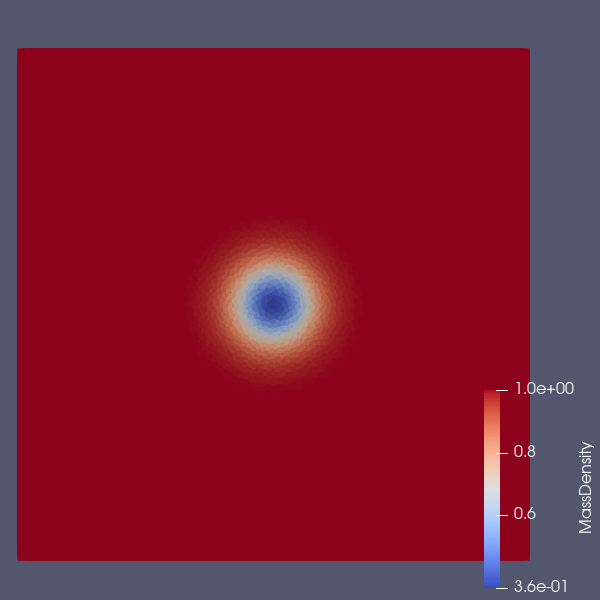
\includegraphics[width=0.47\textwidth]{vortex1.png}
} \hfill
\subcaptionbox{LLS1 reconstruction ($t = 1$).} {
	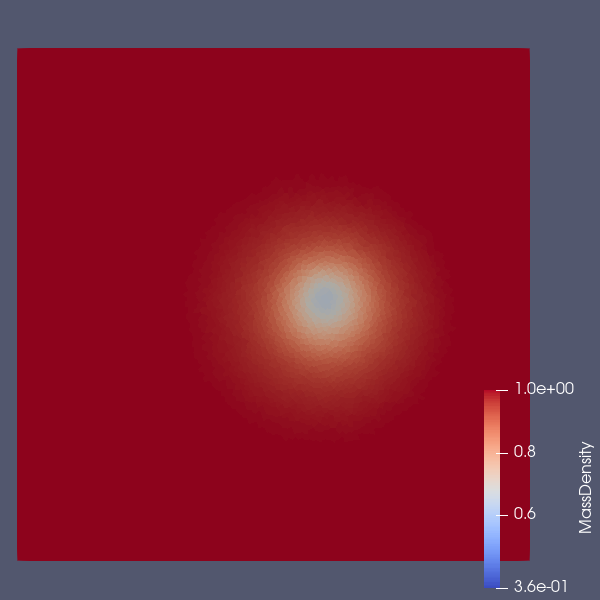
\includegraphics[width=0.47\textwidth]{vortex2.png}
} \\[2em]
\subcaptionbox{LLS2 reconstruction ($t = 1$).} {
	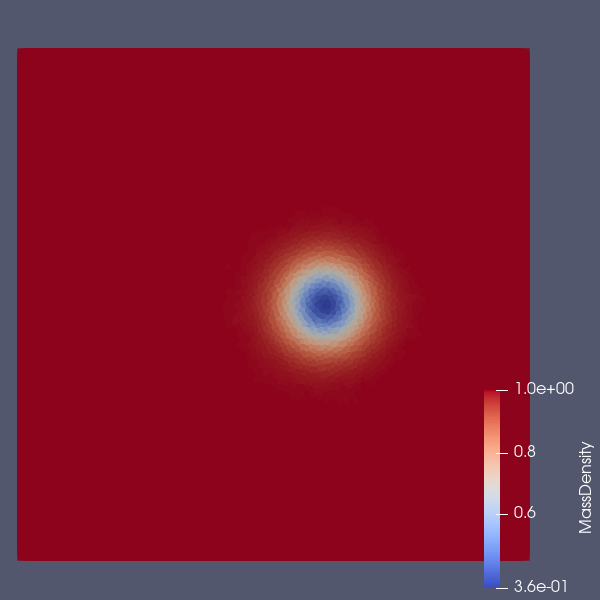
\includegraphics[width=0.47\textwidth]{vortex3.png}
} \hfill
\subcaptionbox{LLS3 reconstruction ($t = 1$).} {
	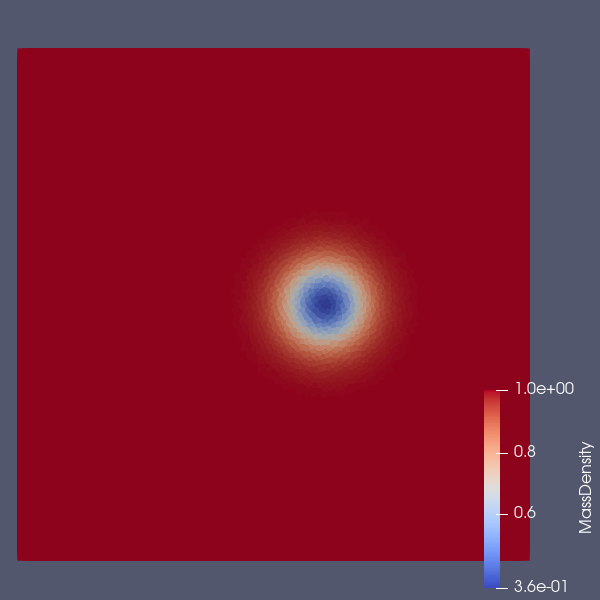
\includegraphics[width=0.47\textwidth]{vortex4.png}
}
\caption{Mass density of the vortex over time.}
\label{fig:comparison-vortex}
\end{figure}

\begin{figure}[p]
\centering
\subcaptionbox{Initial condition ($t = 0$).} {
	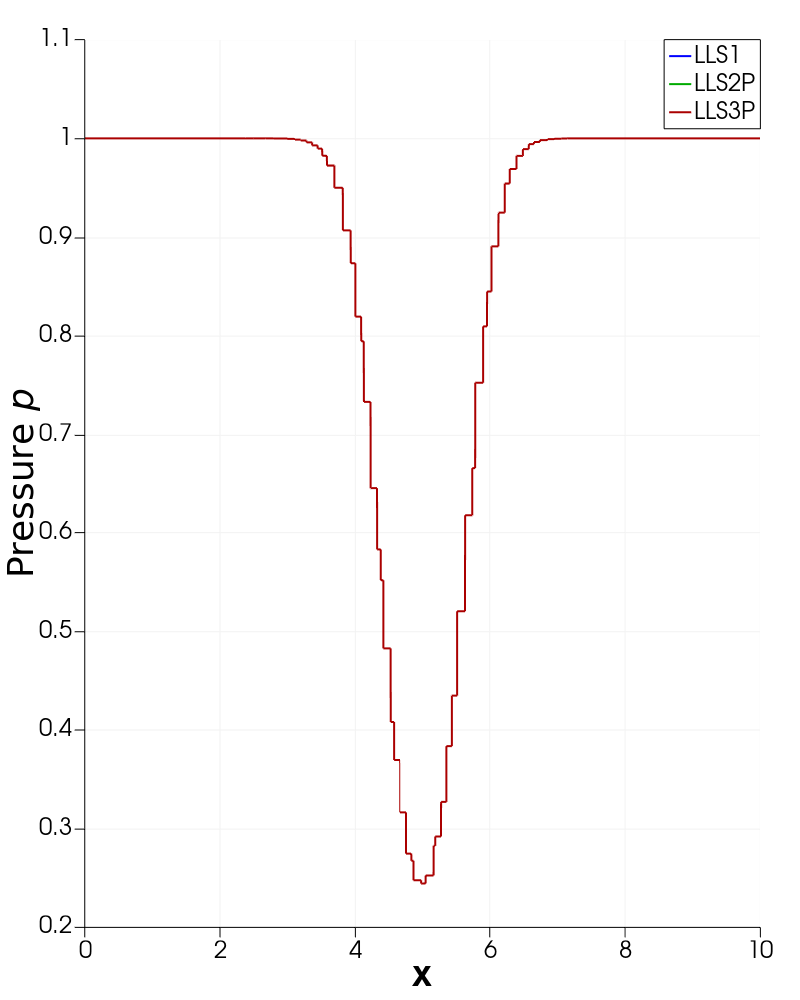
\includegraphics[width=0.47\textwidth]{vortexhor1.png}
} \hfill
\subcaptionbox{Advected vortex ($t = 1$).} {
	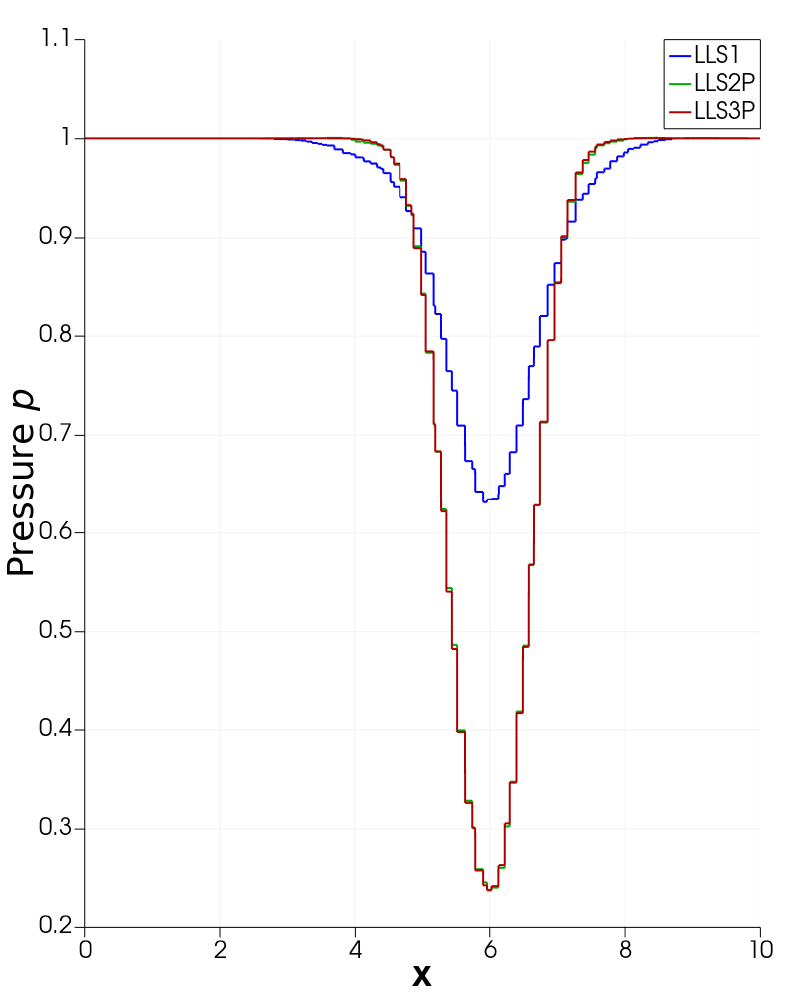
\includegraphics[width=0.47\textwidth]{vortexhor2.png}
}
\caption{Pressure of the vortex over time on the line $y = 0$.}
\label{fig:comparison2-vortex}
\end{figure}

\begin{figure}[p]
\centering
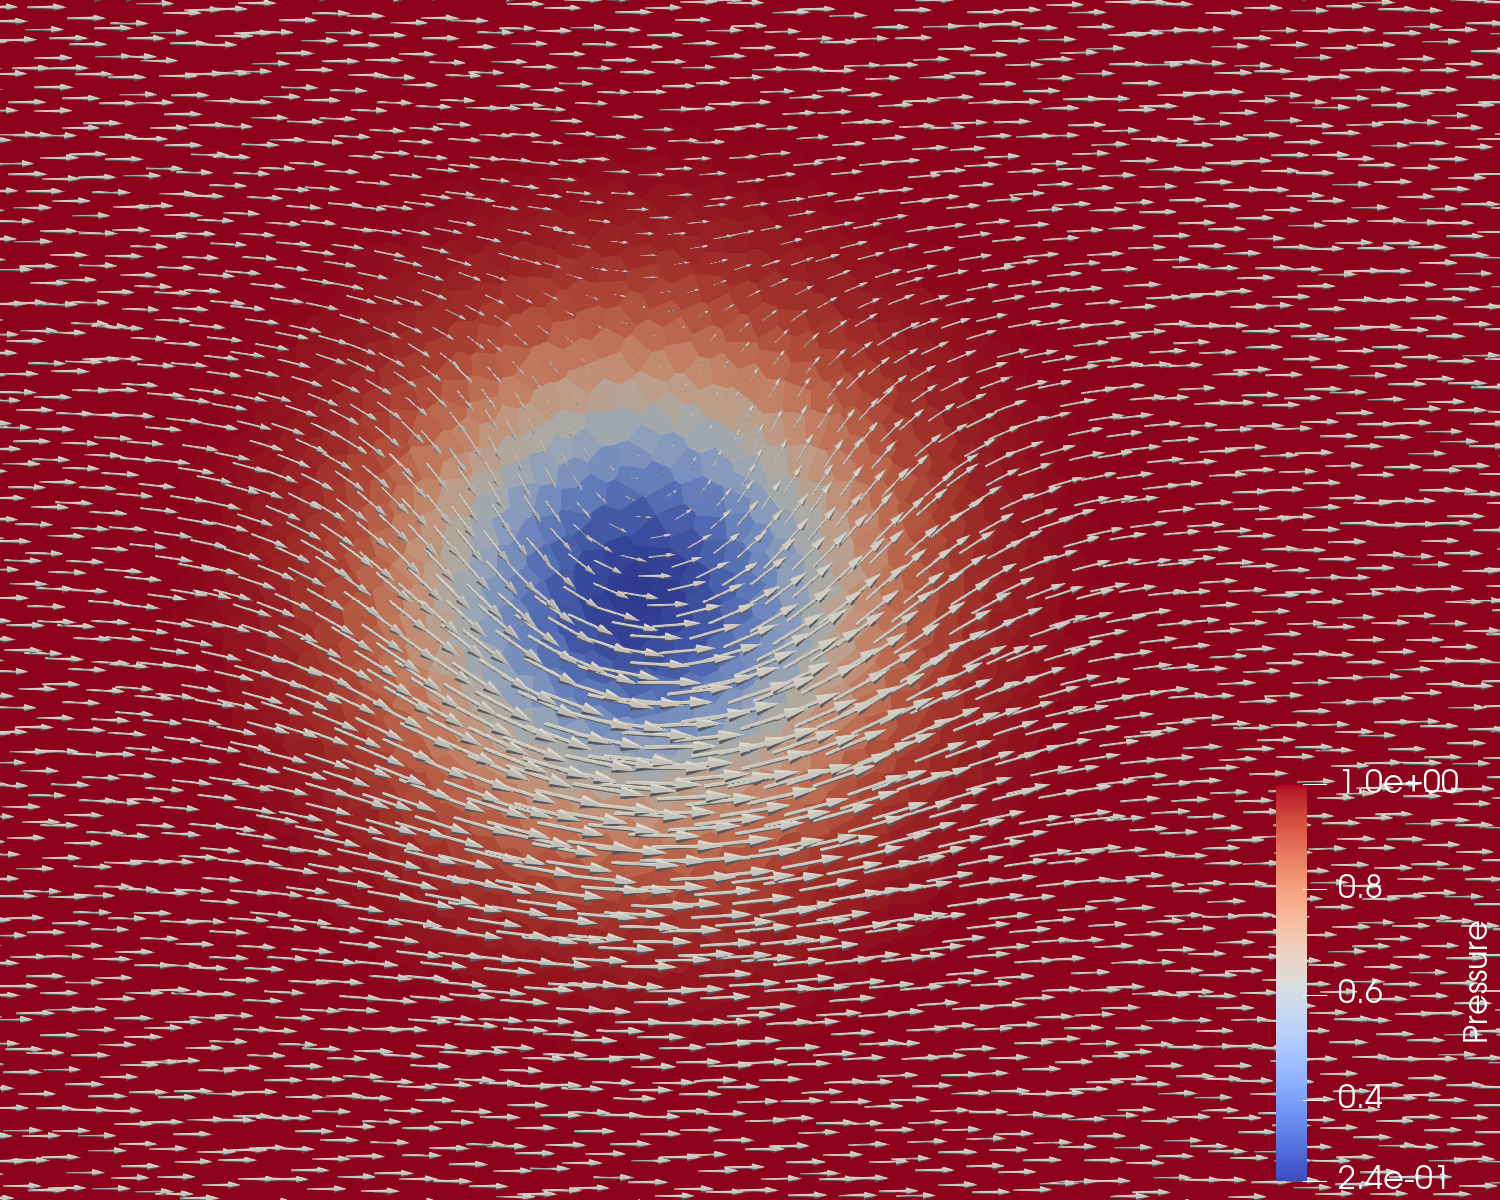
\includegraphics[width=0.9\textwidth]{vortexarrow1.png} \\[2em]
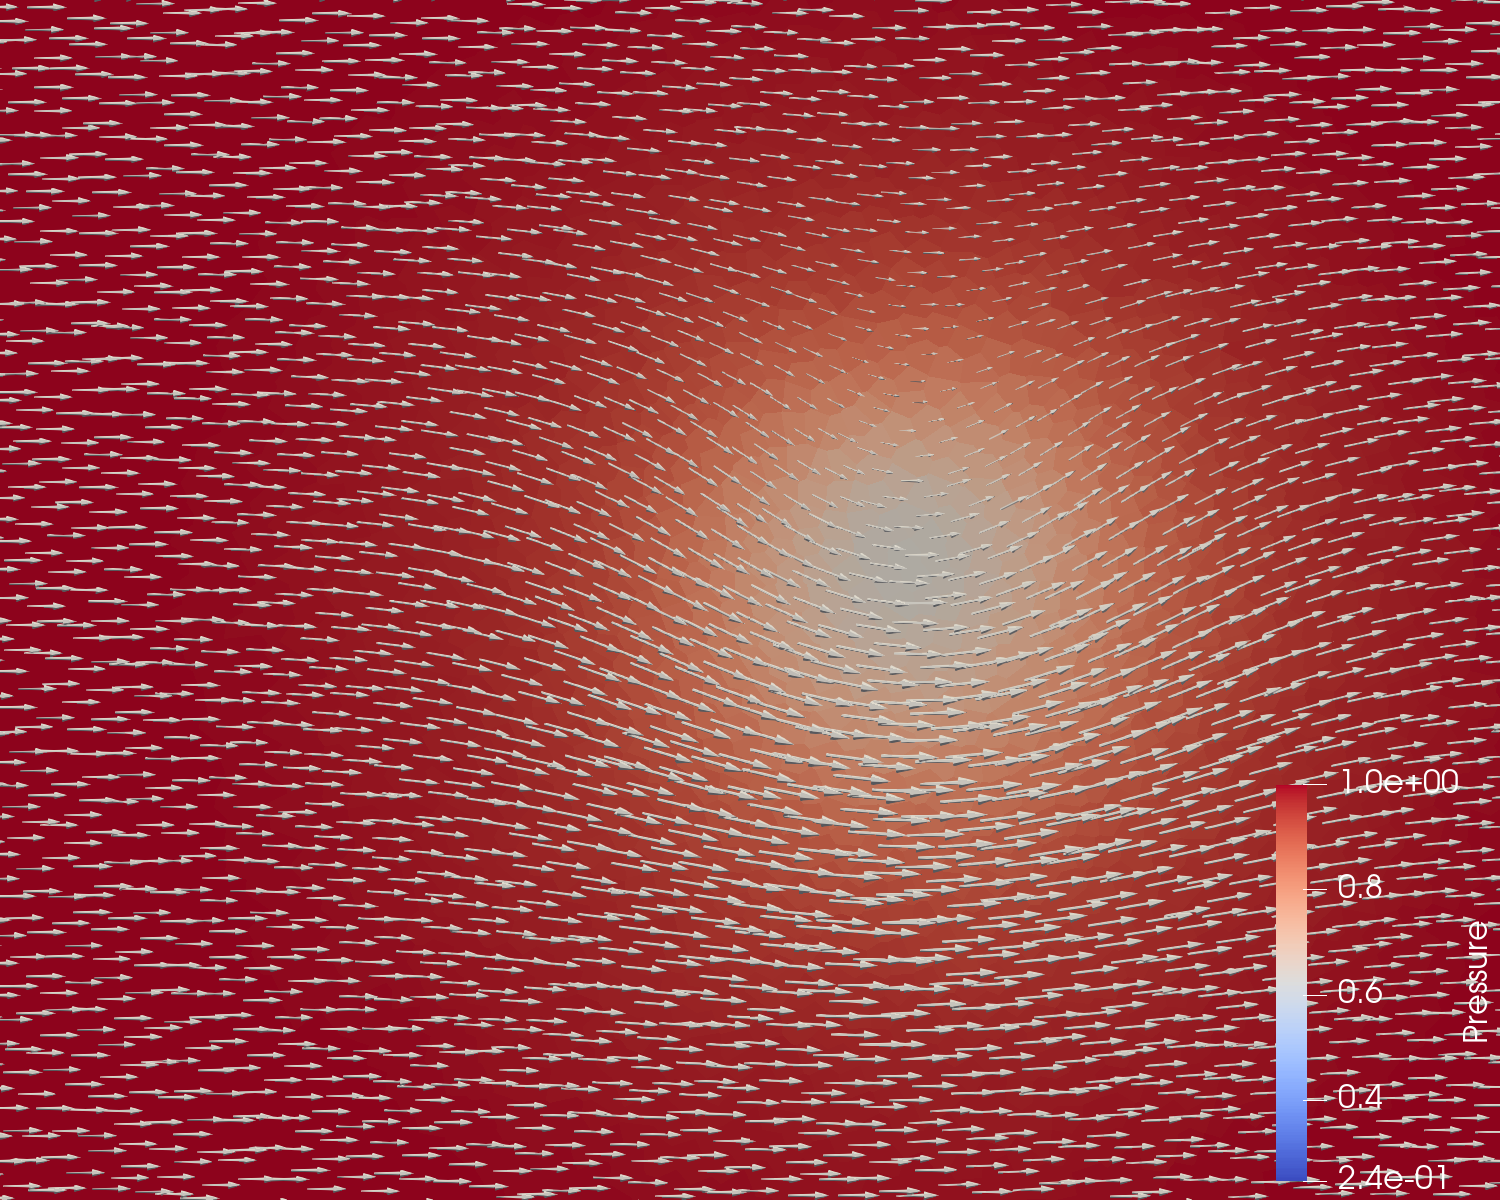
\includegraphics[width=0.9\textwidth]{vortexarrow2.png}
\caption{Attenuation of vortex pressure and velocity by a LLS1 scheme;\\
$t = 0$ above and $t = 1$ below.}
\label{fig:comparison3-vortex}
\end{figure}

\begin{figure}[p]
\centering
\subcaptionbox{Mass density $\rho$.} {
	\begin{tikzpicture}[trim axis left, trim axis right]
	\begin{loglogaxis}[
		xlabel={$h$},
		%ylabel={$L^1$ norm of error on density $\rho$},
		width=0.53\textwidth,
		height=0.4\textheight,
		%ymin=1e-7,
		legend style={anchor=south east,at={(0.975,0.025)}}
	]
	\addplot table[x=h,y=rhoL1] {vortex_regular_LLS1.dat};
	\addplot table[x=h,y=rhoL1] {vortex_regular_LLS2P.dat};
	\addplot table[x=h,y=rhoL1] {vortex_regular_LLS3P.dat};
	\addplot[dashed, domain=0.025:0.2] expression {0.1*x};
	\addplot[dashed, domain=0.025:0.2] expression {0.03*x^2};
	\addplot[dashed, domain=0.025:0.2] expression {0.08*x^3};
	\legend{$\text{LLS1},O(h)$\\$\text{LLS2P},O(h^2)$\\$\text{LLS3P},O(h^3)$\\}
	\end{loglogaxis}
	\end{tikzpicture}
} \hfill
\subcaptionbox{Horizontal momentum $\rho \vec{v}_x$.} {
	\begin{tikzpicture}[trim axis left, trim axis right]
	\begin{loglogaxis}[
		xlabel={$h$},
		%ylabel={$L^1$ norm of error on density $\rho$},
		width=0.53\textwidth,
		height=0.4\textheight,
		%ymin=1e-7,
		legend style={anchor=south east,at={(0.975,0.025)}}
	]
	\addplot table[x=h,y=rhovxL1] {vortex_regular_LLS1.dat};
	\addplot table[x=h,y=rhovxL1] {vortex_regular_LLS2P.dat};
	\addplot table[x=h,y=rhovxL1] {vortex_regular_LLS3P.dat};
	\addplot[dashed, domain=0.025:0.2] expression {0.1*x};
	\addplot[dashed, domain=0.025:0.2] expression {0.08*x^2};
	\addplot[dashed, domain=0.025:0.2] expression {0.2*x^3};
	\legend{$\text{LLS1},O(h)$\\$\text{LLS2P},O(h^2)$\\$\text{LLS3P},O(h^3)$\\}
	\end{loglogaxis}
	\end{tikzpicture}
} \\[2em]
\subcaptionbox{Vertical momentum $\rho \vec{v}_y$.} {
	\begin{tikzpicture}[trim axis left, trim axis right]
	\begin{loglogaxis}[
		xlabel={$h$},
		%ylabel={$L^1$ norm of error on density $\rho$},
		width=0.53\textwidth,
		height=0.4\textheight,
		%ymin=1e-7,
		legend style={anchor=south east,at={(0.975,0.025)}}
	]
	\addplot table[x=h,y=rhovyL1] {vortex_regular_LLS1.dat};
	\addplot table[x=h,y=rhovyL1] {vortex_regular_LLS2P.dat};
	\addplot table[x=h,y=rhovyL1] {vortex_regular_LLS3P.dat};
	\addplot[dashed, domain=0.025:0.2] expression {0.1*x};
	\addplot[dashed, domain=0.025:0.2] expression {0.08*x^2};
	\addplot[dashed, domain=0.025:0.2] expression {0.2*x^3};
	\legend{$\text{LLS1},O(h)$\\$\text{LLS2P},O(h^2)$\\$\text{LLS3P},O(h^3)$\\}
	\end{loglogaxis}
	\end{tikzpicture}
} \hfill
\subcaptionbox{Total energy density $e$.} {
	\begin{tikzpicture}[trim axis left, trim axis right]
	\begin{loglogaxis}[
		xlabel={$h$},
		%ylabel={$L^1$ norm of error on density $\rho$},
		width=0.53\textwidth,
		height=0.4\textheight,
		%ymin=1e-7,
		legend style={anchor=south east,at={(0.975,0.025)}}
	]
	\addplot table[x=h,y=eL1] {vortex_regular_LLS1.dat};
	\addplot table[x=h,y=eL1] {vortex_regular_LLS2P.dat};
	\addplot table[x=h,y=eL1] {vortex_regular_LLS3P.dat};
	\addplot[dashed, domain=0.025:0.2] expression {0.2*x};
	\addplot[dashed, domain=0.025:0.2] expression {0.15*x^2};
	\addplot[dashed, domain=0.025:0.2] expression {0.3*x^3};
	\legend{$\text{LLS1},O(h)$\\$\text{LLS2P},O(h^2)$\\$\text{LLS3P},O(h^3)$\\}
	\end{loglogaxis}
	\end{tikzpicture}
}
\caption{In each plot: $L^1$ norm of the error on the specified
conserved variable.}
\label{fig:comparison-L1-errors-entropy-vortex-regular-grid}
\end{figure}

\begin{figure}[p]
\centering
\subcaptionbox{Mass density $\rho$.} {
	\begin{tikzpicture}[trim axis left, trim axis right]
	\begin{loglogaxis}[
		xlabel={$h$},
		%ylabel={$L^1$ norm of error on density $\rho$},
		width=0.53\textwidth,
		height=0.4\textheight,
		%ymin=1e-7,
		legend style={anchor=south east,at={(0.975,0.025)}}
	]
	\addplot table[x=h,y=rhoLinf] {vortex_regular_LLS1.dat};
	\addplot table[x=h,y=rhoLinf] {vortex_regular_LLS2P.dat};
	\addplot table[x=h,y=rhoLinf] {vortex_regular_LLS3P.dat};
	\addplot[dashed, domain=0.025:0.2] expression {2*x};
	\addplot[dashed, domain=0.025:0.2] expression {0.7*x^2};
	\addplot[dashed, domain=0.025:0.2] expression {3*x^3};
	\legend{$\text{LLS1},O(h)$\\$\text{LLS2P},O(h^2)$\\$\text{LLS3P},O(h^3)$\\}
	\end{loglogaxis}
	\end{tikzpicture}
} \hfill
\subcaptionbox{Horizontal momentum $\rho \vec{v}_x$.} {
	\begin{tikzpicture}[trim axis left, trim axis right]
	\begin{loglogaxis}[
		xlabel={$h$},
		%ylabel={$L^1$ norm of error on density $\rho$},
		width=0.53\textwidth,
		height=0.4\textheight,
		%ymin=1e-7,
		legend style={anchor=south east,at={(0.975,0.025)}}
	]
	\addplot table[x=h,y=rhovxLinf] {vortex_regular_LLS1.dat};
	\addplot table[x=h,y=rhovxLinf] {vortex_regular_LLS2P.dat};
	\addplot table[x=h,y=rhovxLinf] {vortex_regular_LLS3P.dat};
	\addplot[dashed, domain=0.025:0.2] expression {3*x};
	\addplot[dashed, domain=0.025:0.2] expression {1.5*x^2};
	\addplot[dashed, domain=0.025:0.2] expression {7*x^3};
	\legend{$\text{LLS1},O(h)$\\$\text{LLS2P},O(h^2)$\\$\text{LLS3P},O(h^3)$\\}
	\end{loglogaxis}
	\end{tikzpicture}
} \\[2em]
\subcaptionbox{Vertical momentum $\rho \vec{v}_y$.} {
	\begin{tikzpicture}[trim axis left, trim axis right]
	\begin{loglogaxis}[
		xlabel={$h$},
		%ylabel={$L^1$ norm of error on density $\rho$},
		width=0.53\textwidth,
		height=0.4\textheight,
		%ymin=1e-7,
		legend style={anchor=south east,at={(0.975,0.025)}}
	]
	\addplot table[x=h,y=rhovyLinf] {vortex_regular_LLS1.dat};
	\addplot table[x=h,y=rhovyLinf] {vortex_regular_LLS2P.dat};
	\addplot table[x=h,y=rhovyLinf] {vortex_regular_LLS3P.dat};
	\addplot[dashed, domain=0.025:0.2] expression {3*x};
	\addplot[dashed, domain=0.025:0.2] expression {1.5*x^2};
	\addplot[dashed, domain=0.025:0.2] expression {7*x^3};
	\legend{$\text{LLS1},O(h)$\\$\text{LLS2P},O(h^2)$\\$\text{LLS3P},O(h^3)$\\}
	\end{loglogaxis}
	\end{tikzpicture}
} \hfill
\subcaptionbox{Total energy density $e$.} {
	\begin{tikzpicture}[trim axis left, trim axis right]
	\begin{loglogaxis}[
		xlabel={$h$},
		%ylabel={$L^1$ norm of error on density $\rho$},
		width=0.53\textwidth,
		height=0.4\textheight,
		%ymin=1e-7,
		legend style={anchor=south east,at={(0.975,0.025)}}
	]
	\addplot table[x=h,y=eLinf] {vortex_regular_LLS1.dat};
	\addplot table[x=h,y=eLinf] {vortex_regular_LLS2P.dat};
	\addplot table[x=h,y=eLinf] {vortex_regular_LLS3P.dat};
	\addplot[dashed, domain=0.025:0.2] expression {10*x};
	\addplot[dashed, domain=0.025:0.2] expression {5*x^2};
	\addplot[dashed, domain=0.025:0.2] expression {20*x^3};
	\legend{$\text{LLS1},O(h)$\\$\text{LLS2P},O(h^2)$\\$\text{LLS3P},O(h^3)$\\}
	\end{loglogaxis}
	\end{tikzpicture}
}
\caption{In each plot: $L^{\infty}$ norm of the error on the specified
conserved variable.}
\label{fig:comparison-Linf-errors-entropy-vortex-regular-grid}
\end{figure}

%\begin{figure}[p]
%\centering
%\subcaptionbox{$L^1$ norm of the error on a square grid.} {
%	\begin{tikzpicture}[trim axis left, trim axis right]
%	\begin{loglogaxis}[
%		xlabel={$h$},
%		%ylabel={$L^1$ norm of error on density $\rho$},
%		width=0.53\textwidth,
%		height=0.4\textheight,
%		ymin=1e-6, ymax=1e-1,
%		legend style={anchor=south east,at={(0.975,0.025)}}
%	]
%	\addplot table[x=h,y=rhoL1] {waves_regular_LLS1.dat};
%	\addplot table[x=h,y=rhoL1] {waves_regular_LLS2P.dat};
%	\addplot table[x=h,y=rhoL1] {waves_regular_LLS3P.dat};
%	\addplot[dashed, domain=0.025:0.2] expression {0.15*x};
%	\addplot[dashed, domain=0.025:0.2] expression {0.07*x^2};
%	\addplot[dashed, domain=0.025:0.2] expression {0.2*x^3};
%	\legend{$\text{LLS1},O(h)$\\$\text{LLS2P},O(h^2)$\\$\text{LLS3P},O(h^3)$\\}
%	\end{loglogaxis}
%	\end{tikzpicture}
%} \hfill
%\subcaptionbox{$L^1$ norm of the error on a Voronoi grid.} {
%	\begin{tikzpicture}[trim axis left, trim axis right]
%	\begin{loglogaxis}[
%		xlabel={$h$},
%		%ylabel={$L^1$ norm of error on density $\rho$},
%		width=0.53\textwidth,
%		height=0.4\textheight,
%		ymin=1e-6, ymax=1e-1,
%		legend style={anchor=south east,at={(0.975,0.025)}}
%	]
%	\addplot table[x=h,y=rhovxL1] {waves_voronoi_LLS1.dat};
%	\addplot table[x=h,y=rhovxL1] {waves_voronoi_LLS2P.dat};
%	\addplot table[x=h,y=rhovxL1] {waves_voronoi_LLS3P.dat};
%	\addplot[dashed, domain=0.025:0.2] expression {0.15*x};
%	\addplot[dashed, domain=0.025:0.2] expression {0.07*x^2};
%	\addplot[dashed, domain=0.025:0.2] expression {0.2*x^3};
%	\legend{$\text{LLS1},O(h)$\\$\text{LLS2P},O(h^2)$\\$\text{LLS3P},O(h^3)$\\}
%	\end{loglogaxis}
%	\end{tikzpicture}
%} \\[2em]
%\subcaptionbox{$L^{\infty}$ norm of the error on a square grid.} {
%	\begin{tikzpicture}[trim axis left, trim axis right]
%	\begin{loglogaxis}[
%		xlabel={$h$},
%		%ylabel={$L^1$ norm of error on density $\rho$},
%		width=0.53\textwidth,
%		height=0.4\textheight,
%		ymin=1e-6, ymax=1e-1,
%		legend style={anchor=south east,at={(0.975,0.025)}}
%	]
%	\addplot table[x=h,y=rhovyLinf] {waves_regular_LLS1.dat};
%	\addplot table[x=h,y=rhovyLinf] {waves_regular_LLS2P.dat};
%	\addplot table[x=h,y=rhovyLinf] {waves_regular_LLS3P.dat};
%	\addplot[dashed, domain=0.025:0.2] expression {0.25*x};
%	\addplot[dashed, domain=0.025:0.2] expression {0.1*x^2};
%	\addplot[dashed, domain=0.025:0.2] expression {0.4*x^3};
%	\legend{$\text{LLS1},O(h)$\\$\text{LLS2P},O(h^2)$\\$\text{LLS3P},O(h^3)$\\}
%	\end{loglogaxis}
%	\end{tikzpicture}
%} \hfill
%\subcaptionbox{$L^{\infty}$ norm of the error on a Voronoi grid.} {
%	\begin{tikzpicture}[trim axis left, trim axis right]
%	\begin{loglogaxis}[
%		xlabel={$h$},
%		%ylabel={$L^1$ norm of error on density $\rho$},
%		width=0.53\textwidth,
%		height=0.4\textheight,
%		ymin=1e-6, ymax=1e-1,
%		legend style={anchor=south east,at={(0.975,0.025)}}
%	]
%	\addplot table[x=h,y=eLinf] {waves_voronoi_LLS1.dat};
%	\addplot table[x=h,y=eLinf] {waves_voronoi_LLS2P.dat};
%	\addplot table[x=h,y=eLinf] {waves_voronoi_LLS3P.dat};
%	\addplot[dashed, domain=0.025:0.2] expression {0.25*x};
%	\addplot[dashed, domain=0.025:0.2] expression {0.1*x^2};
%	\addplot[dashed, domain=0.025:0.2] expression {0.4*x^3};
%	\legend{$\text{LLS1},O(h)$\\$\text{LLS2P},O(h^2)$\\$\text{LLS3P},O(h^3)$\\}
%	\end{loglogaxis}
%	\end{tikzpicture}
%}
%\caption{Errors in the entropy waves test. All conserved variables give the
%same errors, so only mass density $\rho$ is shown.}
%\label{fig:comparison-errors-entropy-waves}
%\end{figure}
































\graphicspath{{./figures/chapter4/}}
\lstset{inputpath = ../MATLAB}
\pgfplotstableset{search path = ./tables/chapter4}

\chapter{WENO reconstructions} \label{ch:WENO}

The reconstruction strategy based on least squares polynomial interpolation
that was introduced in Chapter \ref{ch:FVM} relies on a key technical assumption
about the exact solution $\vec{u}(\vec{x},t)$ of a hyperbolic system
of conservation laws: its smoothness in the neighborhood of every cell.
As we have seen in Section \ref{sec:conservation-laws}, however,
smooth solutions can develop discontinuities in finite time,
so it is necessary to investigate the behavior of these methods
when applied to discontinuous data, too.

On the one hand, the least squares system $\mat{V}_i \, \vec{p}_i = \bar{\vec{u}}$
is still well-defined even if the stencil $S_i$ of a cell $C_i$ crosses
a discontinuity, because the Vandermonde matrix $\mat{V}_i$ doesn't depend
on $\bar{\vec{u}}$. Hence, $\vec{p}_i$ can still be computed and evaluated
at $\vec{x}_{ijk}$ as before.

On the other hand, there is no guarantee that $\vec{p}_i(\vec{x}_{ijk})$
is an accurate approximation of $\vec{u}(\vec{x}_{ijk})$ anymore,
because error terms in a Taylor expansion of $\vec{u}$ don't hold
across a discontinuity. In the field of approximation theory, it is
well known that using the polynomial space $\Pi_K$ to approximate discontinuous
data is a bad idea, as undesired oscillations are produced in the neighborhood
of any discontinuity. This is exactly what happens when the methods
of the previous chapter are applied to the simulation of nonsmooth flows.

If the jumps in the cell averages $\bar{\vec{u}}_i$ are small enough,
LLS-$K$ methods can still produce quantitatively acceptable results,
despite their oscillatory behavior near the discontinuities.
For larger jumps, however, it may happen that $\vec{p}_i$ oscillates
so much that $\vec{p}_i(\vec{x}_{ijk}) \notin \mathcal{U}$, with $\mathcal{U}$
being the set of admissible values for a solution $\vec{u}(\vec{x},t)$
as defined at the end of Section \ref{sec:derivation-euler}.
For example, in the case of the compressible Euler equations, it may happen
that either the density or the pressure of a reconstruction on the border
of some cell becomes negative, and at that point there is no meaningful
way to continue the simulation.
This is exactly what happens when a LLS-$K$ reconstruction with $K \geq 2$
is used to solve the Riemann problem
\begin{equation} \label{eq:sod-shock-tube}
\vec{u}(x,y,0) = 
\begin{cases}
(1,0,0,(\gamma-1)^{-1}) &\text{if $x < 1/2$} \\
(1/8,0,0,(1/10)(\gamma-1)^{-1}) &\text{if $x \geq 1/2$} \\
\end{cases}
\end{equation}
for the 2D compressible Euler equations on the domain $[0,1] \times [0,1]$,
which is a standard test for the numerical solution of the compressible
Euler equations known as Sod's shock tube problem \cite{sod1978survey}.
The breakdown of the finite volume method was confirmed by a numerical
simulation; Programs \ref{prog:check-state2D} and \ref{prog:check-edges-state2D}
illustrate the MATLAB code that is used to check the admissibility
of the cell averages and of the reconstructions over the course of the simulation.

In the literature, numerous techniques have been developed to combine
high-order schemes with nonoscillatory behavior near discontinuities.
Among them, one of the most popular, versatile and effective technique
is Weighted Essentially NonOscillatory (WENO) approximation,
first introduced for one-dimensional problems by Liu, Osher and Chan in 1994 as an
improvement over earlier ENO interpolation \cite{liu1994weighted}.
Later, WENO reconstructions were generalized to 2D problems on triangular
meshes by Hu and Shu \cite{hu1999weighted}.
For an introduction to WENO schemes and all of its possible
applications in the field of approximation theory, we refer
to the very accessible review article by Shu \cite{shu2009high}.
For the classical theory of WENO schemes on tensor product grids,
we refer to Shu's lecture notes \cite{cockburn2006advanced}
and to Chapter 11 of the recent book by Hestaven \cite{hesthaven2017numerical}.

The main idea behind WENO reconstructions is to choose multiple
interpolation stencils $S_{i\ell}$ on every cell $C_i$, so that different
least squares polynomial reconstructions $\vec{p}_{i\ell}(\vec{x})$ are defined,
and then to take as an approximation of $\vec{u}(\vec{x},t)$ on $\partial C_i$
a convex combination
\begin{equation} \label{eq:WENO-convex-combination}
\vec{p}_i = \sum_{\ell} \omega_{i\ell} \, \vec{p}_{i\ell}
\end{equation}
of all polynomials $\vec{p}_{i\ell}$, each one weighted by a coefficient
$\omega_{i\ell}$ that depends on a \emph{smoothness indicator}
$S\!I(\vec{p}_{i\ell})$ (a better name would be \emph{oscillation functional},
but this is how it is known in the literature).
In this way, oscillatory reconstructions are penalized, and all that is needed
to get an essentially nonoscillatory reconstruction is to have at least one
nonoscillatory polynomial~$\vec{p}_{i\bar{\ell}}$ in the convex combination
\eqref{eq:WENO-convex-combination}.
To achieve this, one-sided stencils that span different directions are used
in addition to a centered stencil like that of Chapter \ref{ch:FVM}:
if the strategy is successful, at least one of the stencils will not cross
a discontinuity and will therefore produce the required nonoscillatory
polynomial~$\vec{p}_{i\bar{\ell}}$.
Since the weights $\omega_{i\ell}$ depend nonlinearly on $\vec{p}_{i\ell}$,
and hence nonlinearly on $\bar{\vec{u}}_i(t)$, WENO schemes are
said to be \emph{nonlinear schemes}, unlike the LLS-$K$ schemes
of Chapter \ref{ch:FVM}.

In \cite{liu2013robust}, Liu and Zhang introduced the distinction
between type-I and type-II WENO interpolations.
The first type consists of WENO reconstructions whose order of accuracy is
not higher than that of the reconstruction on each stencil.
For this type of WENO reconstruction, the nonlinear weights do not
contribute towards the increase of the order of accuracy, because they are
designed purely for the purpose of nonlinear stability and to avoid
spurious oscillations in the numerical solution.
We remark that a convex combination like \eqref{eq:WENO-convex-combination}
of $K$-exact reconstructions $\vec{p}_{i\ell}$ is itself a $K$-exact
reconstruction, so type-I WENO schemes have order $K$ if the
exact solution $\vec{u}(\vec{x},t)$ is sufficiently smooth.

The second type consists of WENO reconstructions whose order of accuracy in regions
where $\vec{u}(\vec{x},t)$ is smooth is higher than that of the reconstruction
on each stencil, typically by a factor of 1.
For example, a third order type-II WENO interpolation on a 2D mesh can be
based on second order linear polynomial reconstructions on each stencil.
For this type of WENO reconstruction, the nonlinear weights contribute
towards the increase of the order of accuracy, because the overall
reconstruction is given at each quadrature node $\vec{x}_{ijk}$ by a weighted
average of the lower order reconstructions (in this case, the weights
$\omega_{i\ell}$ must depend on the indices $j$ and $k$ in addition to $i$ and $\ell$).

In the next section we propose a generalization of type-I WENO reconstructions
to arbitrary polygonal meshes. This is something that, to the best of our
knowledge, has never been tried before; our first results are encouraging.

\section{Type-I WENO reconstructions on polygonal meshes}
Suppose that on each cell $C_i$ a collection
$\{S_{i\ell}\}_{\ell = 1 \dots N_S(i)}$ of $N_S(i)$ distinct stencils
has been defined, and let $m_{i\ell}$ be the size of each stencil $S_{i\ell}$.
Let $\vec{p}_{i\ell}$ be the polynomial of degree $K$ obtained by
the least squares procedure of Chapter \ref{ch:FVM} from the cell averages
$\{\bar{\vec{u}}_\kappa \mid \kappa \in S_{i\ell}\}$.
Then, we define our type-I WENO reconstruction by the convex combination
\begin{equation} \label{eq:WENO}
\vec{p}_i = \sum_{\ell} \omega_{i\ell} \, \vec{p}_{i\ell},
\end{equation}
which is evaluated on every quadrature node $\vec{x}_{ijk}$ of cell $C_i$
to produce either $\vec{u}_{ijk}^+$ or $\vec{u}_{ijk}^-$, depending on whether
the normal $\vec{\nu}_{ij}$ points into $C_i$ or away from $C_i$, respectively.
The weights $\omega_{i\ell}$ are obtained by normalizing another set
of strictly positive weights $\tilde{\omega}_{i\ell}$:
\[
\omega_{i\ell} = \frac{\tilde{\omega}_{i\ell}}
                      {\sum_{\ell=1}^{N_S(i)} \tilde{\omega}_{i\ell}}.
\]
It is these weights $\tilde{\omega}_{i\ell}$ that, as anticipated,
depend on the smoothness indicator $S\!I(\vec{p})$. This indicator should give
us an estimate of how strongly a polynomial $\vec{p}$ oscillates on $C_i$;
a standard choice for $S\!I(\vec{p})$ is to define it as the sum of the squares
of the $L^2$ norms of all the derivatives of $\vec{p}$ of order 1 to $K$:
\[
S\!I(\vec{p}) \deq \sum_{1 \leq \abs{\alpha} \leq K} \frac{1}{\abs{C_i}}
	\int_{C_i} h_i^{2\abs{\alpha}} \bigl(\partial_\alpha \vec{p}(x,y)\bigr)^2 \dxy
\]
The sum is taken over a two-dimensional multi-index $\alpha$.
The terms $\abs{C_i}^{-1}\!$ and $h_i^{2\abs{\alpha}}$ are introduced
to make the smoothness indicator scale-invariant with respect to the
size of $C_i$.
% Under the assumption of shape regularity
%(see Definition \ref{defi:shape-regularity}),
This can be proved by switching to the same local coordinates $(\xi,\eta)$
that were used in Chapter \ref{ch:FVM} to keep the condition number
of the least squares system bounded as $h \to 0$.
%\[
%(\xi,\eta) \deq \left( \frac{x-x_i}{h_i}, \frac{y-y_i}{h_i} \right)
%\qquad \varphi(x,y) \deq \left( \frac{x-x_i}{h_i}, \frac{y-y_i}{h_i} \right)
%\quad \varphi \colon C_i \to \hat{C}_i
%\]
%with $(x_i,y_i)$ barycenter of cell $C_i$.

As in every WENO scheme, the unnormalized weights $\tilde{\omega}_{i\ell}$
are then defined by
\begin{equation} \label{eq:unnormalized-weights}
\tilde{\omega}_{i\ell} = \frac{c_\ell}{(\varepsilon + S\!I(\vec{p}_{i\ell}))^r}
\qquad \varepsilon,r > 0.
\end{equation}
We now see why oscillating reconstructions are penalized: for any
polynomial $\vec{p}_{i\ell}$, a larger value of the functional
$S\!I(\vec{p}_{i\ell})$ corresponds to a smaller unnormalized weight
$\tilde{\omega}_{i\ell}$.
The coefficients $c_\ell > 0$ are known as \emph{linear coefficients} of the
reconstruction, and if dependent on $j$ and $k$ provide type-II WENO
schemes the necessary degrees of freedom to achieve higher orders of convergence.
Since we are only dealing with type-I WENO reconstructions in this work,
we can simply take $c_\ell = 1$ for all $\ell = 1, \dots, N_S(i)$,
on the principle that equally oscillating polynomials should
get the same weights in formula \eqref{eq:WENO}.

The parameters $\varepsilon$ and $r$ in \eqref{eq:unnormalized-weights}
can be tuned depending on the problem that has to be solved.
The parameter $\varepsilon$ is a small positive number used to avoid division by zero.
$S\!I(\vec{p}_{i\ell}) = 0$ if and only if $\vec{p}_{i\ell}$ is a constant
polynomial, so smaller values of $\varepsilon$ emphasize the fact
that constant reconstructions are assigned larger weights compared
to nonconstant ones.
The positive exponent $r$ controls the sensitivity of the unnormalized weights
with respect to the oscillation indicator. When $r \to \infty$, the reconstruction
$\vec{p}_i$ converges to the least oscillating polynomial among
$\{\vec{p}_{i\ell}\}_{\ell = 1 \dots N_S(i)}$,
whereas for $r \to 0$ the reconstruction $\vec{p}_i$ converges to the
arithmetic mean of all the polynomials $\{\vec{p}_{i\ell}\}_{\ell = 1 \dots N_S(i)}$.
In practice, the choices $\varepsilon = 10^{-6}$ and $r = 4$ give satisfactory
results for most problems.

\subsection*{Choice of stencils}
As we have already pointed out in the introduction to this chapter,
WENO reconstructions are nonoscillatory only if at least one of the
stencils $S_{i\ell}$ does not cross a discontinuity.
Therefore, it makes sense in this context to consider stencils
that look like circular sectors rather than circles: in this way,
even if a cell $C_i$ is right next to a shock, we can find a stencil
that points in the opposite direction of the shock, and that stencil
should give us the nonoscillatory reconstruction that we are looking for.

To make this idea mathematically precise, let us denote the barycenter
of each cell $C_i$ with $\vec{x}_i$, and let
$A(\vec{x}_i,\vec{x}_\ell,\vec{x}_\kappa)$ be the angle in $\R^2$
formed by the left and right rays
\[
\{ \vec{x}_i + \tau (\vec{x}_\ell - \vec{x}_i) \mid \tau \geq 0 \},
\qquad
\{ \vec{x}_i + \tau (\vec{x}_\kappa - \vec{x}_i) \mid \tau \geq 0 \}.
\]
Then, for each cell $C_i$ and for each pair $C_\mu, C_\lambda$
of adjacent cells in consecutive counterclockwise order with respect
to $C_i$, we would like to define a one-sided stencil $S_{i\ell}$
that covers a region of $\R^2$ with a shape that resembles
$A(\vec{x}_i,\vec{x}_\lambda,\vec{x}_\mu)$ as much as possible.
The idea is to once again consider the adjacency graph $G$ of the given
tessellation $\mathcal{T}_h$ and define the set
\[
D_A(C_i,r) = \{ C_\ell
	\mid d(C_i,C_\ell) \leq r \text{ and } C_\ell \cap A \neq \emptyset\}
\]
as the collection of all cells in $\mathcal{T}_h$ that have graph distance
at most $r$ from $C_i$ and that touch a given angle $A$. Let $n_i$ be the
dimension of the polynomial space $\Pi_K$. Then, for each pair $C_\mu, C_\lambda$
of adjacent cells in consecutive counterclockwise order with respect
to $C_i$, our heuristic is to define $S_{i\ell}$ as the set
$D_{A(\vec{x}_i,\vec{x}_\lambda,\vec{x}_\mu)}(C_i,\bar{r})$,
with $\bar{r} \in \N$ being the smallest non-negative integer such that
$D_{A(\vec{x}_i,\vec{x}_\lambda,\vec{x}_\mu)}(C_i,\bar{r})$ has at least
$n_i$ elements.

\begin{figure}[tbp]
\centering
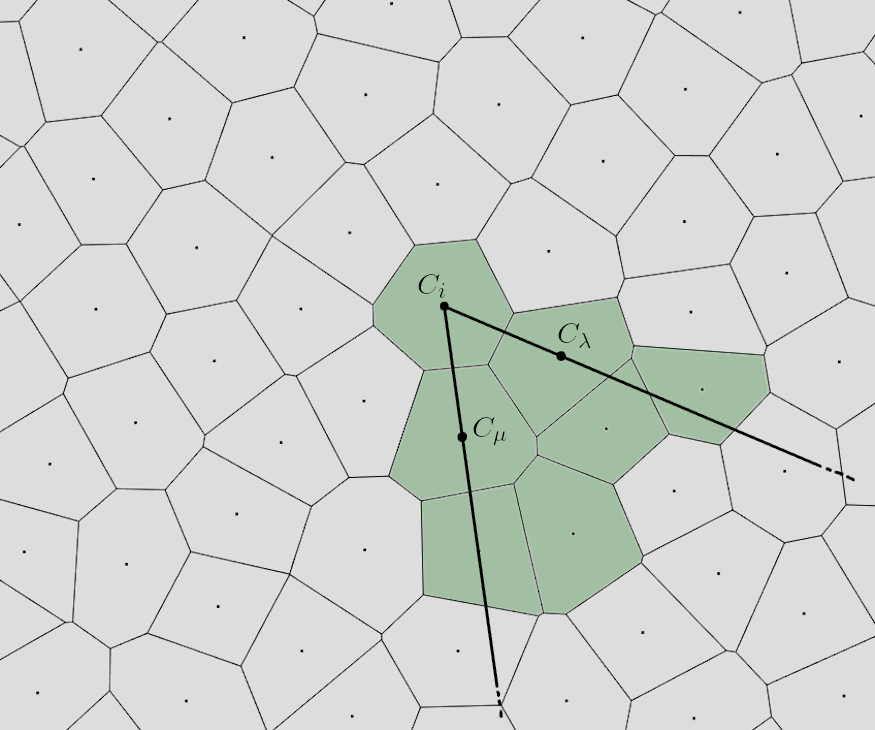
\includegraphics[width=0.48\textwidth]{cellsWENO1.png}
\hfill
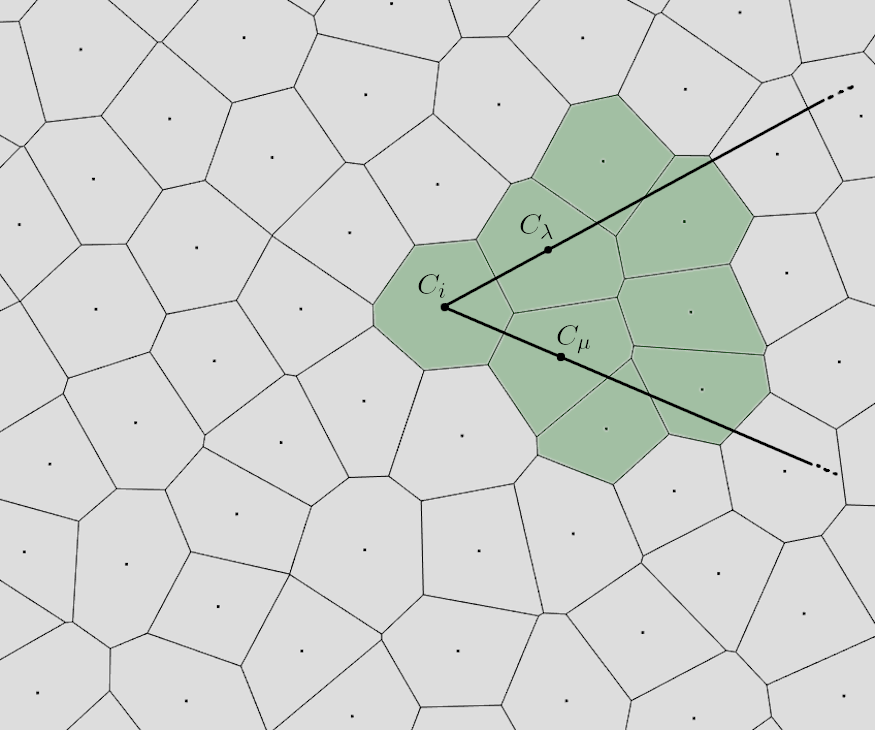
\includegraphics[width=0.48\textwidth]{cellsWENO2.png}
\caption{Examples of one-sided stencils for quadratic WENO reconstructions.}
\label{fig:stencils}
\end{figure}

\subsection*{Implementation details}
Once again, the stencils $S_{i\ell}$ can be efficiently computed
by a breadth-first search algorithm on the graph $G$ with starting node
$C_i$ and with the angle $A(\vec{x}_i,\vec{x}_\lambda,\vec{x}_\mu)$
working as a kind of filter on the cells, as implemented in the
\code{C++} function \code{build\_onesided\_stencil()} contained in
Program \ref{prog:reconstruction}.
Figure \ref{fig:stencils} shows some typical outputs of this algorithm.
Green cells belong to the one-sided stencils, while gray cells do not;
the barycenters $\vec{x}_i, \vec{x}_\lambda, \vec{x}_\mu$ are highlighted.

WENO reconstructions of order $K$ up to 3 are implemented in
Program \ref{prog:reconstruction-T1WENO}. The condition number
of $\mat{V}_{i\ell}$, even if bounded by switching to local coordinates
$(\xi,\eta)$, could be much higher for a one-sided stencil compared to
a centered stencil. Therefore, while solving the least squares problem
in function \code{least\_squares\_and\_condition\_number} of Program
\ref{prog:reconstruction} we use the LAPACK routine \code{DTRCON}
on the upper-triangular factor R of the QR decomposition
of $\mat{V}_{i\ell}$: in this way, we get almost for free an estimate
on the condition number of $\mat{V}_{i\ell}$ and, if it is above
a certain threshold, we remove the polynomial $\vec{p}_{i\ell}$ from
the convex combination \eqref{eq:WENO-convex-combination}.
Just to make sure that we do not discard all stencils, we always include
in \eqref{eq:WENO-convex-combination} the polynomial reconstruction
given by a centered stencil (the same as in LLS-$K$ schemes).

The numerical treatment of boundary conditions that we have
seen in Section \ref{sec:boundary-condtions} is also adequate
for WENO schemes; the only difference is that, for added robustness
when a planar shock wave hits a wall, we progressively reduce the order
of the WENO scheme next to the boundary of the domain.

\section{Numerical tests in the nonsmooth case}

\subsection*{Sod's shock tube problem}
As a first test, we solve Sod's shock tube problem
\eqref{eq:sod-shock-tube} using WENO reconstructions of increasing order.
The domain $\Omega = [0,1] \times [0,1]$ is discretized with
a 512$\times$512 square grid. Since the Riemann problem
described by \eqref{eq:sod-shock-tube} is essentially
a 2D extension of a 1D problem, we put periodic boundary conditions
on the top and bottom sides of $\partial\Omega$.
As for the left and right sides, we choose wall boundary conditions,
although this is not really important because we stop the
simulation before any of the perturbations in the fluid can reach
the end of the tube.
If $K = 1$ or $K = 2$, we put one quadrature point on each edge, else two.
An SSPRK method of order $K$ is used for the numerical solution
of the system of ordinary differential equations produced by the
finite volume method. As for WENO parameters, we choose
$\varepsilon = 10^{-12}$ and $r = 4$. Such a small $\varepsilon$
is well-suited for Riemann problems like \eqref{eq:sod-shock-tube},
because we expect large regions of the solution to be constant.

Figure \ref{fig:sod} shows the density of the numerical solution
at time $T = 0.2$ as a function of~$x$ (both the continuous and the discrete
solutions are constant with respect to $y$). The exact solution contains
a rarefaction wave between $x \approx 0.263$ and $x \approx 0.486$,
a contact discontinuity at $x \approx 0.685$, and a shock wave at $x \approx 0.85$.
Figure \ref{fig:sod-closeup} zooms in on the most interesting
parts of the previous figure. We can clearly see that higher order
WENO methods have sharper transitions around discontinuities,
especially the contact discontinuity, but are nevertheless nonoscillatory.
This is exactly the behavior that we hoped to achieve by introducing
WENO reconstructions.

\begin{figure}[p]
\centering
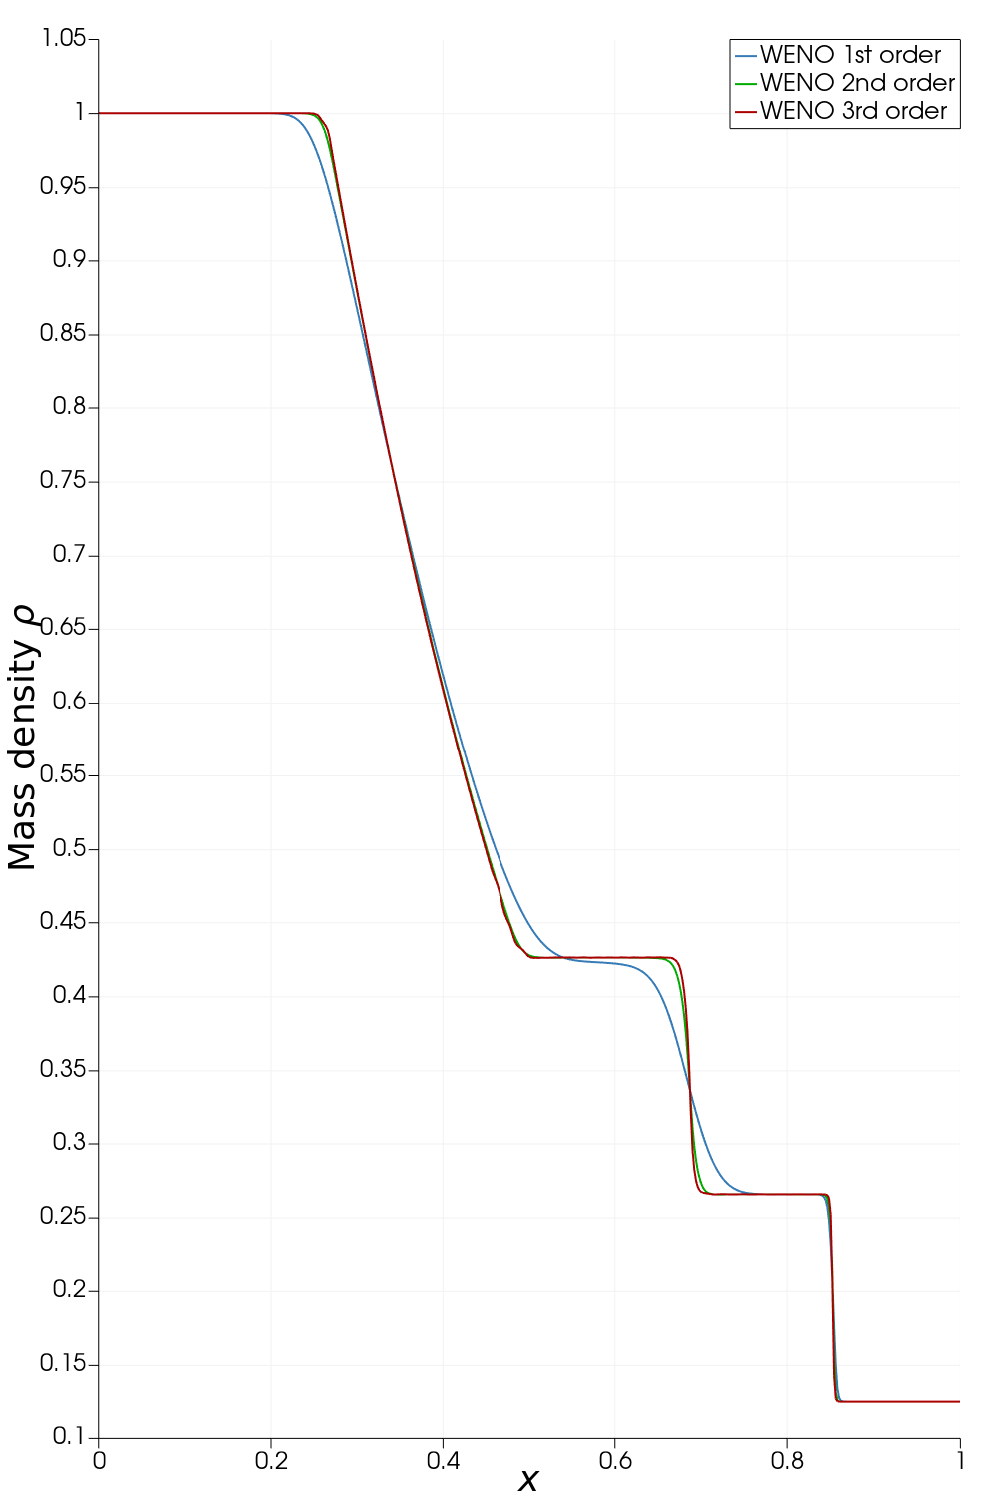
\includegraphics[width=0.98\textwidth]{sod1.png}
\caption{Numerical solution of Sod's shock tube problem at $t = 0.2$.}
\label{fig:sod}
\end{figure}

\begin{figure}[p]
\centering
\subcaptionbox{Left end of the rarefaction wave.} {
	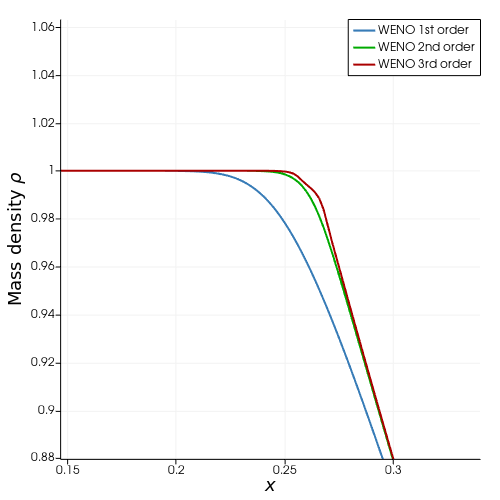
\includegraphics[width=0.47\textwidth]{sod2.png}
} \hfill
\subcaptionbox{Right end of the rarefaction wave.} {
	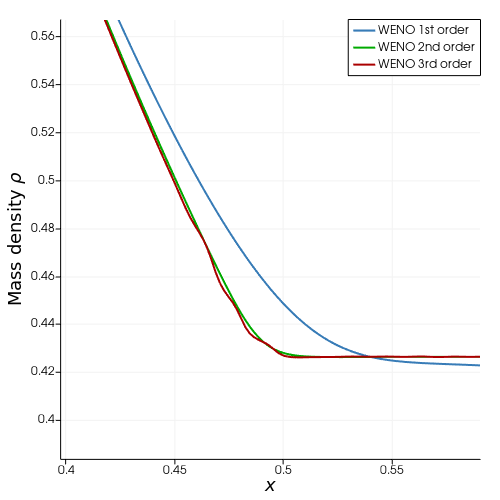
\includegraphics[width=0.47\textwidth]{sod3.png}
} \\[2em]
\subcaptionbox{Contact discontinuity.} {
	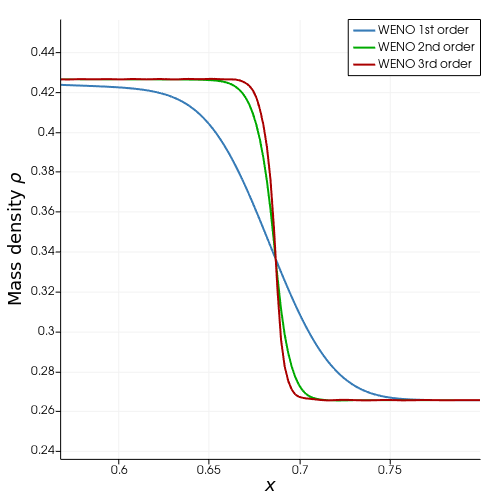
\includegraphics[width=0.47\textwidth]{sod4.png}
} \hfill
\subcaptionbox{Shock wave.} {
	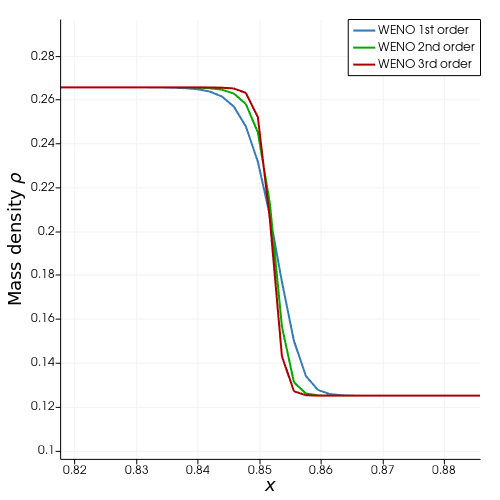
\includegraphics[width=0.47\textwidth]{sod5.png}
}
\caption{Details of the numerical solution of Sod's shock tube problem at $t = 0.2$.}
\label{fig:sod-closeup}
\end{figure}

\subsection*{Elliptical whispering gallery}
Consider an elliptical domain $\Omega$ whose border is defined implicitly
by the equation
\[
\frac{x^2}{a^2} + \frac{y^2}{b^2} = 1,
\]
with semi-major axis $a > 0$ and semi-minor axis $b \in (0,a)$.
Then, the foci $\vec{F}_1, \vec{F}_2$ of the ellipse have coordinates
\[
\vec{F}_1 = (-\sqrt{a^2 - b^2}, 0), \quad \vec{F}_2 = (\sqrt{a^2 - b^2}, 0)
\]
and it is possible to prove that $\partial \Omega$ is the locus
of points $\vec{x}$ in the Euclidean plane such that the sum of the distances
$\norm{\vec{x}-\vec{F}_1}$ and $\norm{\vec{x}-\vec{F}_2}$ is equal to $2a$:
\[
\partial\Omega = \{ \vec{x} \in \R^2 \mid
\norm{\vec{x}-\vec{F}_1} + \norm{\vec{x}-\vec{F}_2} = 2a \}.
\]
An interesting geometrical property of an ellipse is that, for each point
$\vec{x} \in \partial\Omega$, the normal $\vec{\nu}(\vec{x})$ to the
border is a bisector of the angle formed by the rays
\[
\{ \vec{x} + \tau (\vec{F}_1 - \vec{x}) \mid \tau \geq 0 \},
\qquad
\{ \vec{x} + \tau (\vec{F}_2 - \vec{x}) \mid \tau \geq 0 \}.
\]
This in turn implies that the reflection on $\partial\Omega$ of any ray
originating from one of the foci necessarily passes through the other
focus after having traveled a distance $2a$.
An acoustic consequence of this property is that, in an elliptical room
under ideal conditions, a whisper by a person standing at $\vec{F}_1$
will be heard by another person standing at $\vec{F}_2$ regardless
of the distance $2a$: elliptical rooms make excellent whispering galleries.

In this second numerical test, our aim is to reproduce this acoustic
phenomenon using a finite volume scheme based on WENO reconstructions
of order two. For this purpose, we fix an elliptical domain $\Omega$
and simulate the time evolution of a very narrow Gaussian perturbation on
the initial pressure and density fields localized at $\vec{F}_1$.
Let $A$ be the amplitude and $\sigma$ be the width of the Gaussian perturbation.
Then, we consider the following initial conditions for $\vec{u}$, here
expressed in the more convenient variables $(\rho,\vec{v},p)$:
\begin{equation} \label{eq:ellipse-initial-conditions}
\begin{gathered}
\vec{u}_0(\vec{x}) =
\begin{pmatrix}
\rho_\infty  \bigl( 1 + A \exp(-\norm{\vec{x}-\vec{F}_1}/(2\sigma^2) \bigr) \\ 
\vec{v}_\infty \\
p_\infty \bigl( 1 + A \exp(-\norm{\vec{x}-\vec{F}_1}/(2\sigma^2) \bigr)
\end{pmatrix} \\
\rho_\infty = \SI{1,225}{\kg\per\meter\cubed},
\quad \vec{v}_\infty = 0,
\quad p_\infty = \SI{101325}{\pascal},
\quad A = 0.1,
\quad \sigma = 0.2
\end{gathered}
\end{equation}
%The freestream values $(\rho_\infty,\vec{v}_\infty,p_\infty)$ are
The initial condition is smooth, but also very steep in a neighborhood
of $\vec{F}_1$. Since a numerical scheme can hardly distinguish
between discontinuities and very strong gradients in the data,
WENO schemes are required to prevent spurious oscillations
near the wave fronts.
The size of the ellipse $\Omega$ is defined using a Pythagorean triple, so that
\[
a = 29, \quad b = 21, \quad \vec{F}_1 = (-20,0), \quad \vec{F}_2 = (20,0),
\]
and $\Omega$ is discretized by the Voronoi technique explained in
Section \ref{sec:mesh-generation}. Figure \ref{fig:ellipse-2500} shows what a
tessellation of $\Omega$ looks like with $N_c = 1415$; for our simulation we choose
a much finer partition with $N_c = 21599$. Wall boundary conditions
are chosen on the entirety of $\partial\Omega$. Since $K = 2$, a single
quadrature point on each edge will suffice. An SSPRK method of order $2$
is used for the numerical solution of the system of ordinary differential
equations produced by the finite volume method. As for WENO parameters,
we choose $\varepsilon = 10^{-8}$ and $r = 4$.
The speed of sound in the unperturbed fluid is
\[
c_\infty = \sqrt{\frac{\gamma p_\infty}{\rho_\infty}}
\approx \SI{340,3}{\meter\per\second},
\]
therefore we expect the sound waves caused by the perturbation
of the initial data to reach $\vec{F}_2$ after approximately
$t_f \deq 2a/c_\infty \approx \SI{0.17}{\second}$.
Indeed, looking at the results in Figure \ref{fig:ellipse-simulation}
we can see that, after an initial dispersion of the Gaussian perturbation,
the acoustic waves reflect on the walls as expected and eventually
reach $\vec{F}_2$.
Of course, numerical diffusion prevents the spike in pressure
at $\vec{F}_2$ to be as high and localized as it was in the initial
conditions, but it is still significantly higher than every single
wave front at time $t_f/2$, meaning that a simultaneous superposition
of waves was achieved. Figure \ref{fig:ellipse-F2} confirms that the spike
in pressure is exactly at $\vec{x} = (20,0)$, as expected.

The significance of this test is manifold. First of all, the correct
treatment of the wall boundary conditions is checked, since waves
are able to correctly reflect off the walls at every possible angle
of incidence.
Second, the test confirms that waves are traveling at the correct speed,
since they all reach $\vec{F}_2$ at the same time.
Third, the values of pressure are nonoscillatory. Figure
\ref{fig:ellipse-P001} shows a section of the numerical solution
on the horizontal line $y = 0$ at time $t = 0.01$,
and the transition from the wave fronts to the unperturbed fluid
are indeed monotone.
The bump in pressure at $\vec{F}_1$ is not a numerical artifact,
but an actual feature of the exact solution.

\begin{figure}[tbp]
\centering
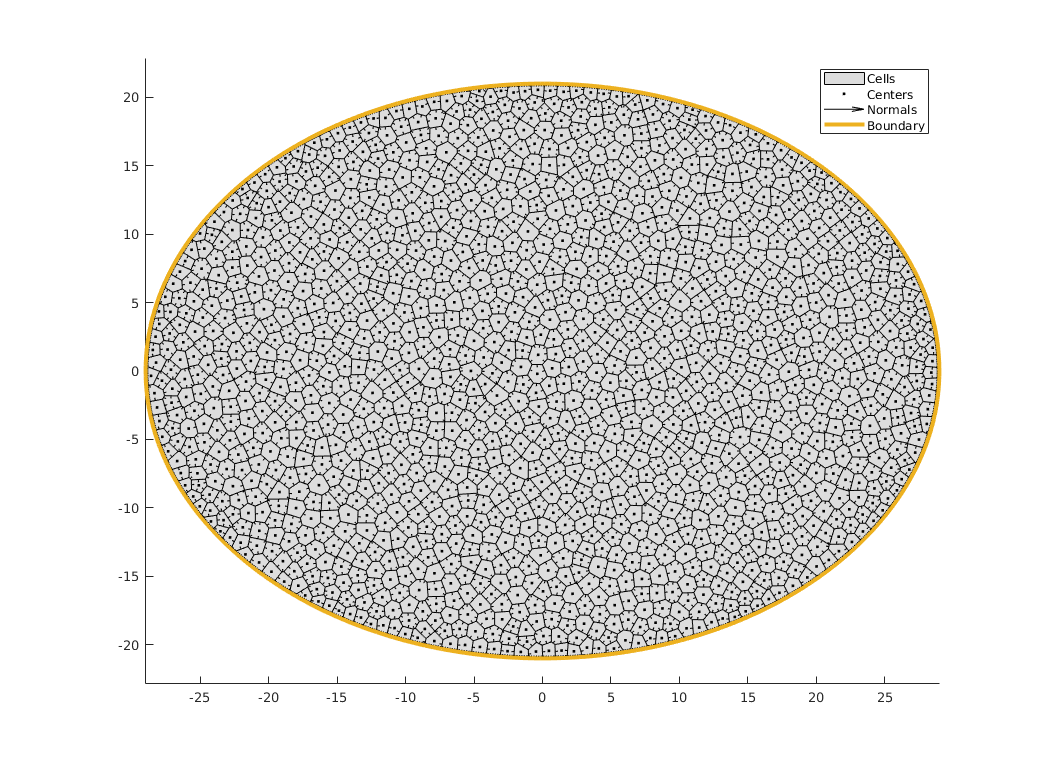
\includegraphics[width=0.8\textwidth]{ellipse2500.png}
\caption{Polygonal discretization of the ellipse, 1415 Voronoi cells.}
\label{fig:ellipse-2500}
\end{figure}

\clearpage

\begin{figure}[p]
\centering
\subcaptionbox{Pressure at $t = 0$} {
	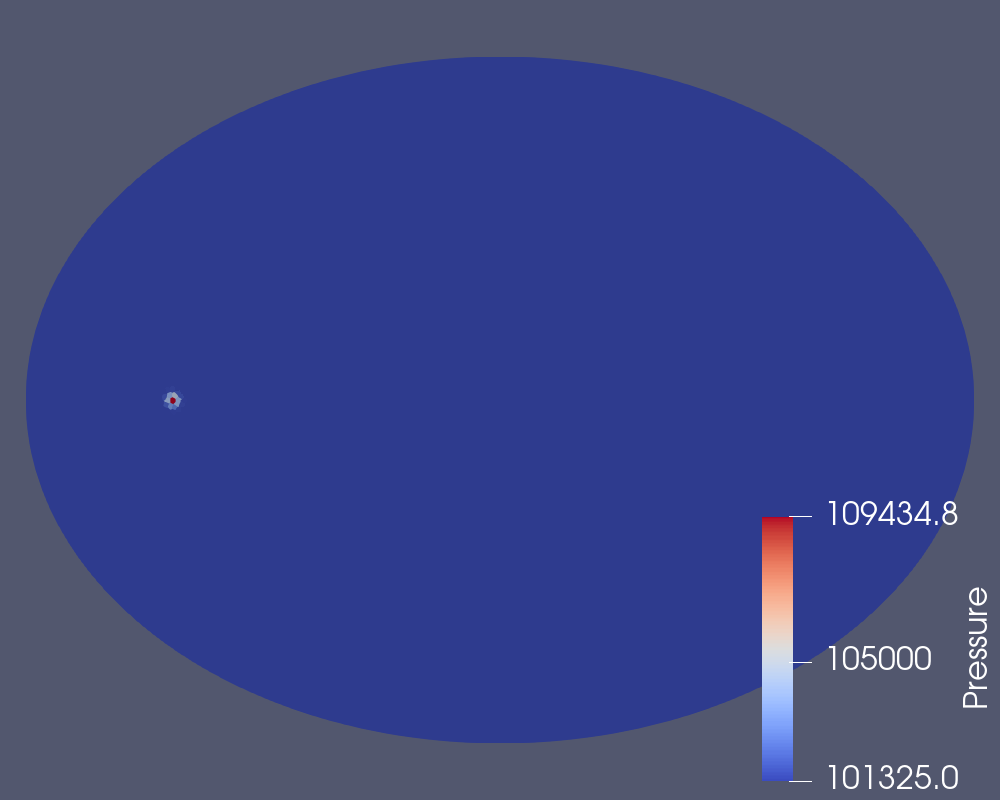
\includegraphics[width=0.47\textwidth]{ellipset0.png}
} \hfill
\subcaptionbox{Pressure at $t = 0.01$} {
	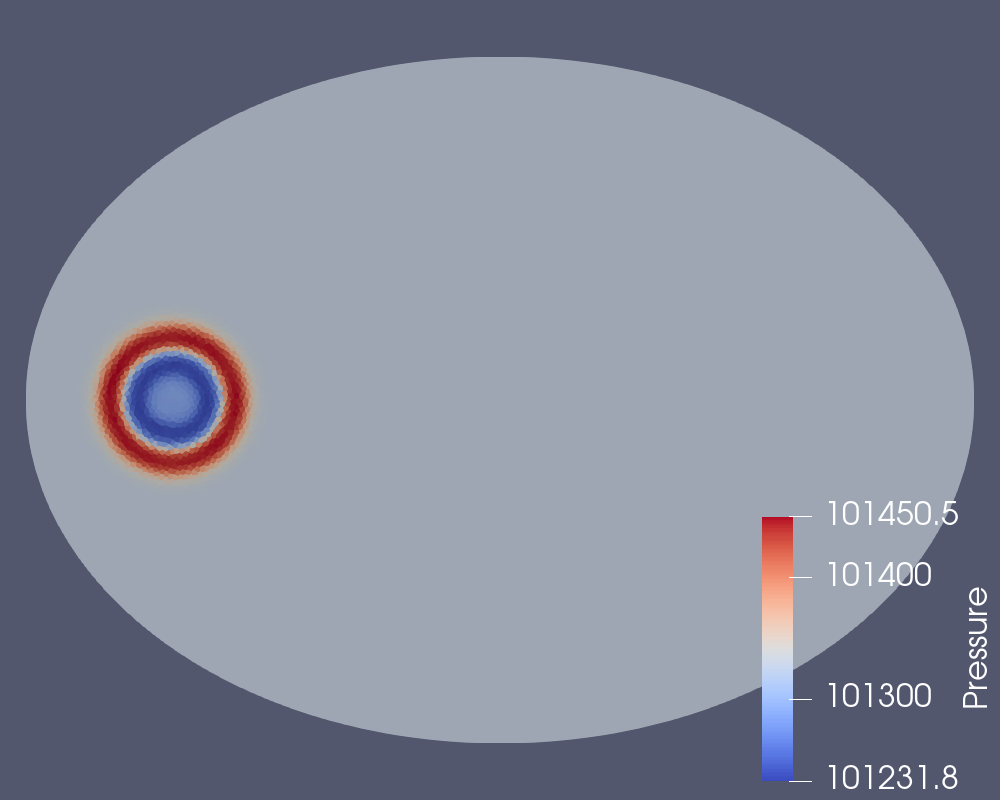
\includegraphics[width=0.47\textwidth]{ellipset001.png}
} \\[2em]
\subcaptionbox{Pressure at $t = 0.05$} {
	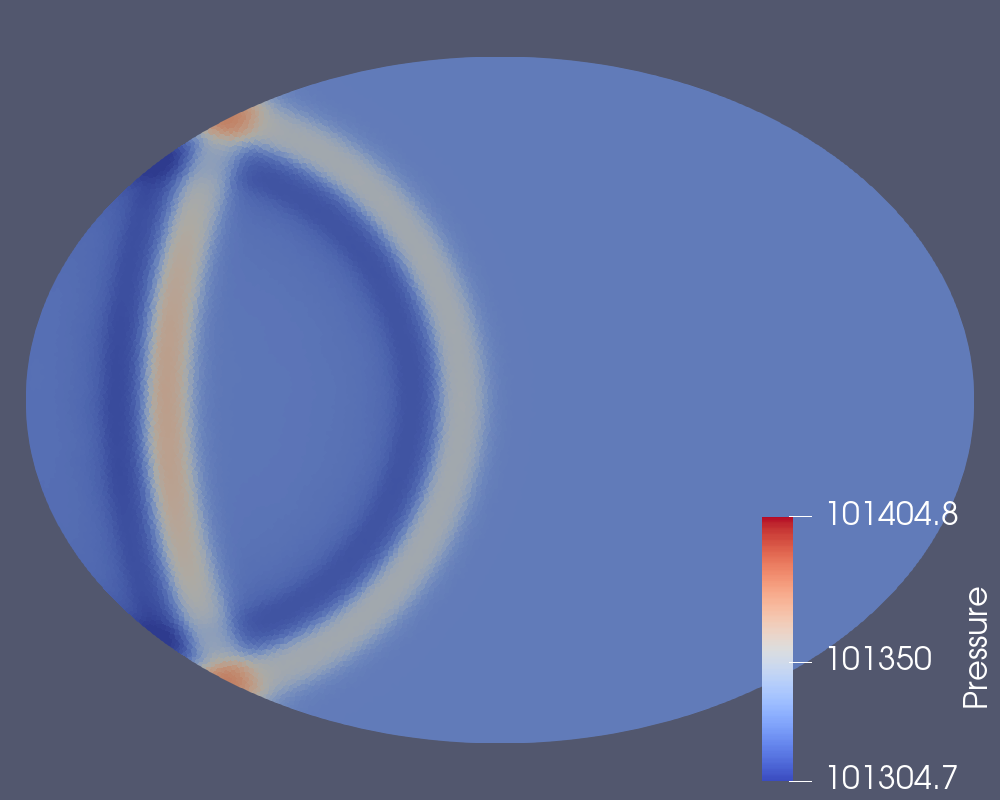
\includegraphics[width=0.47\textwidth]{ellipset005.png}
} \hfill
\subcaptionbox{Pressure at $t = 0.1$} {
	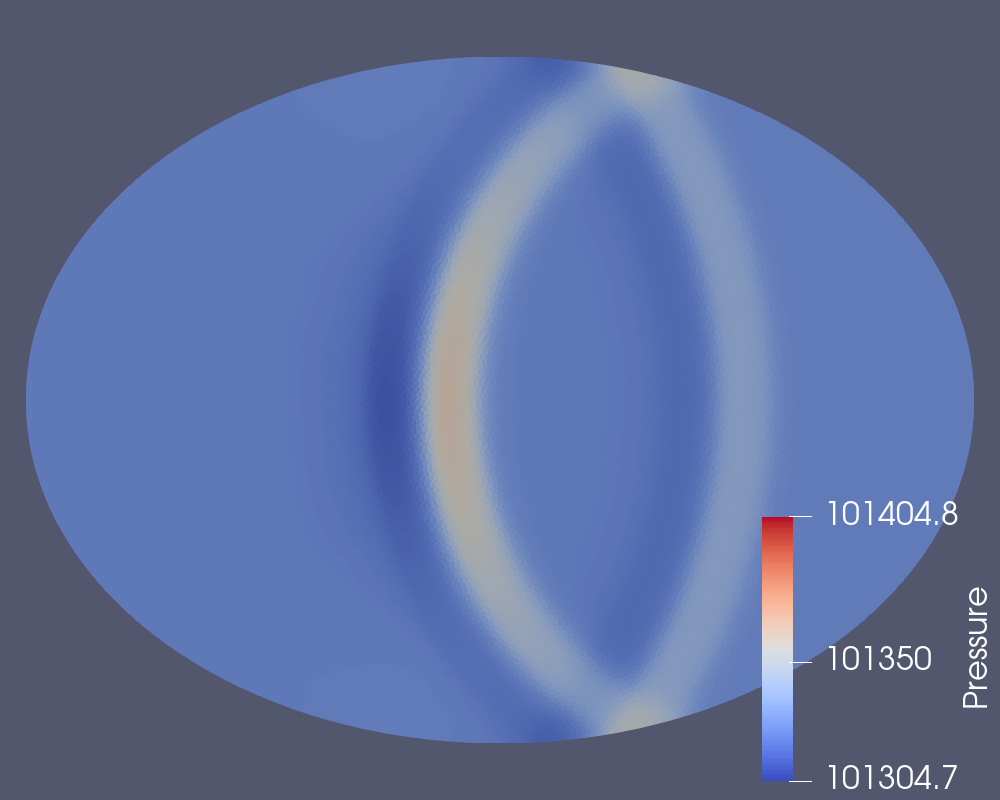
\includegraphics[width=0.47\textwidth]{ellipset010.png}
} \\[2em]
\subcaptionbox{Pressure at $t = 0.15$} {
	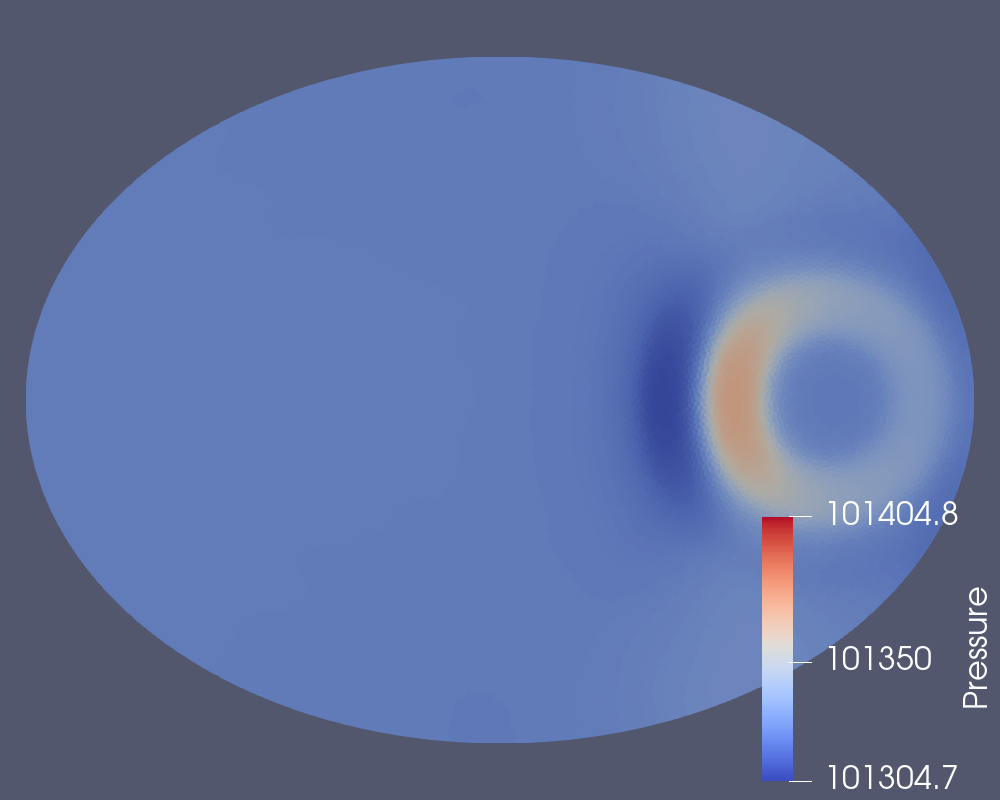
\includegraphics[width=0.47\textwidth]{ellipset015.png}
} \hfill
\subcaptionbox{Pressure at $t = 0.1645$} {
	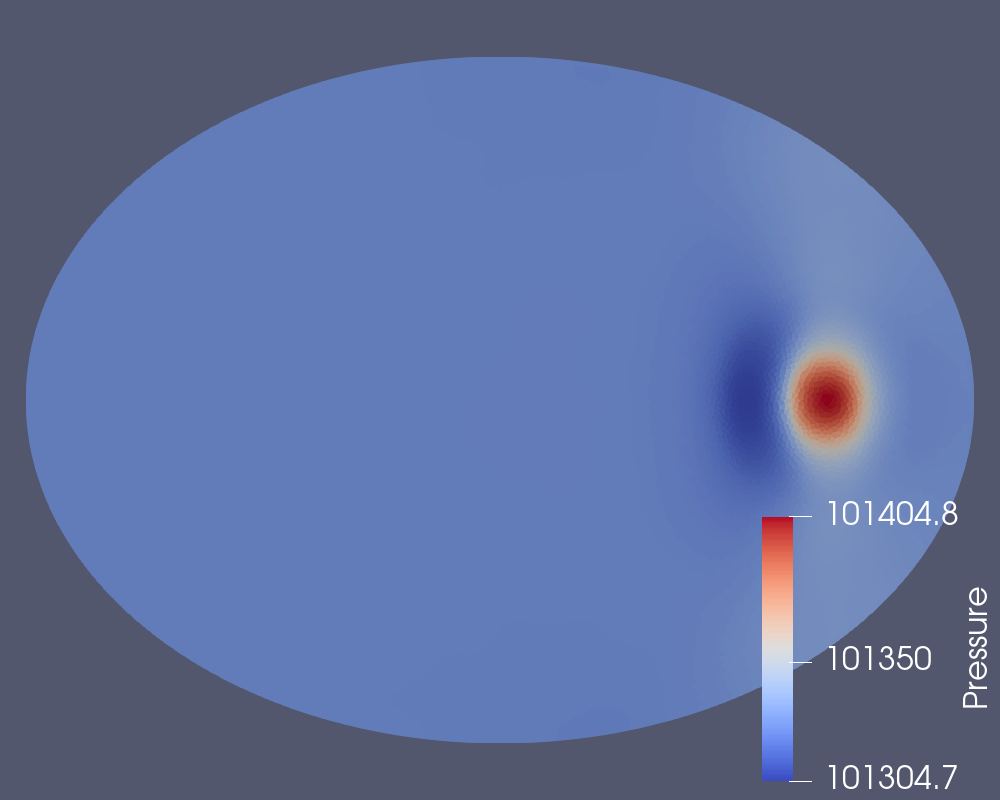
\includegraphics[width=0.47\textwidth]{ellipset01645.png}
}
\caption{Elliptical whispering gallery problem with initial conditions
\eqref{eq:ellipse-initial-conditions}.}
\label{fig:ellipse-simulation}
\end{figure}

\begin{figure}[p]
\centering
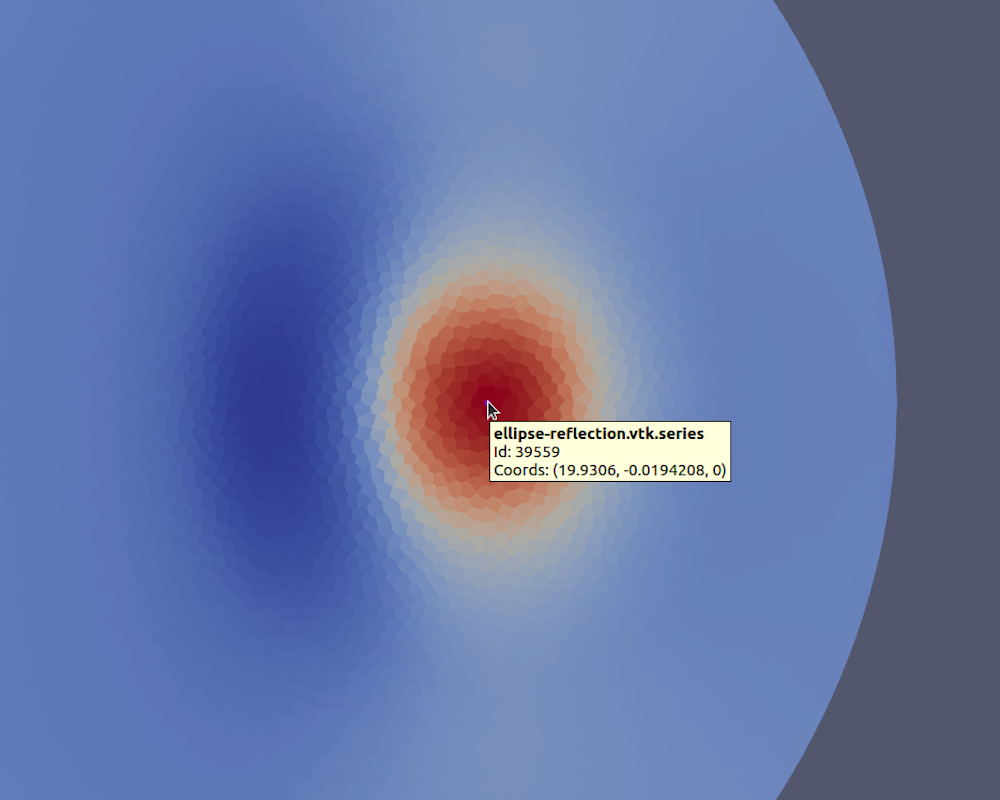
\includegraphics[width=0.65\textwidth]{ellipseF2.png}
\caption{Coordinates of the pressure spike at $t = 0.1645$.}
\label{fig:ellipse-F2}
\end{figure}

\begin{figure}[p]
\centering
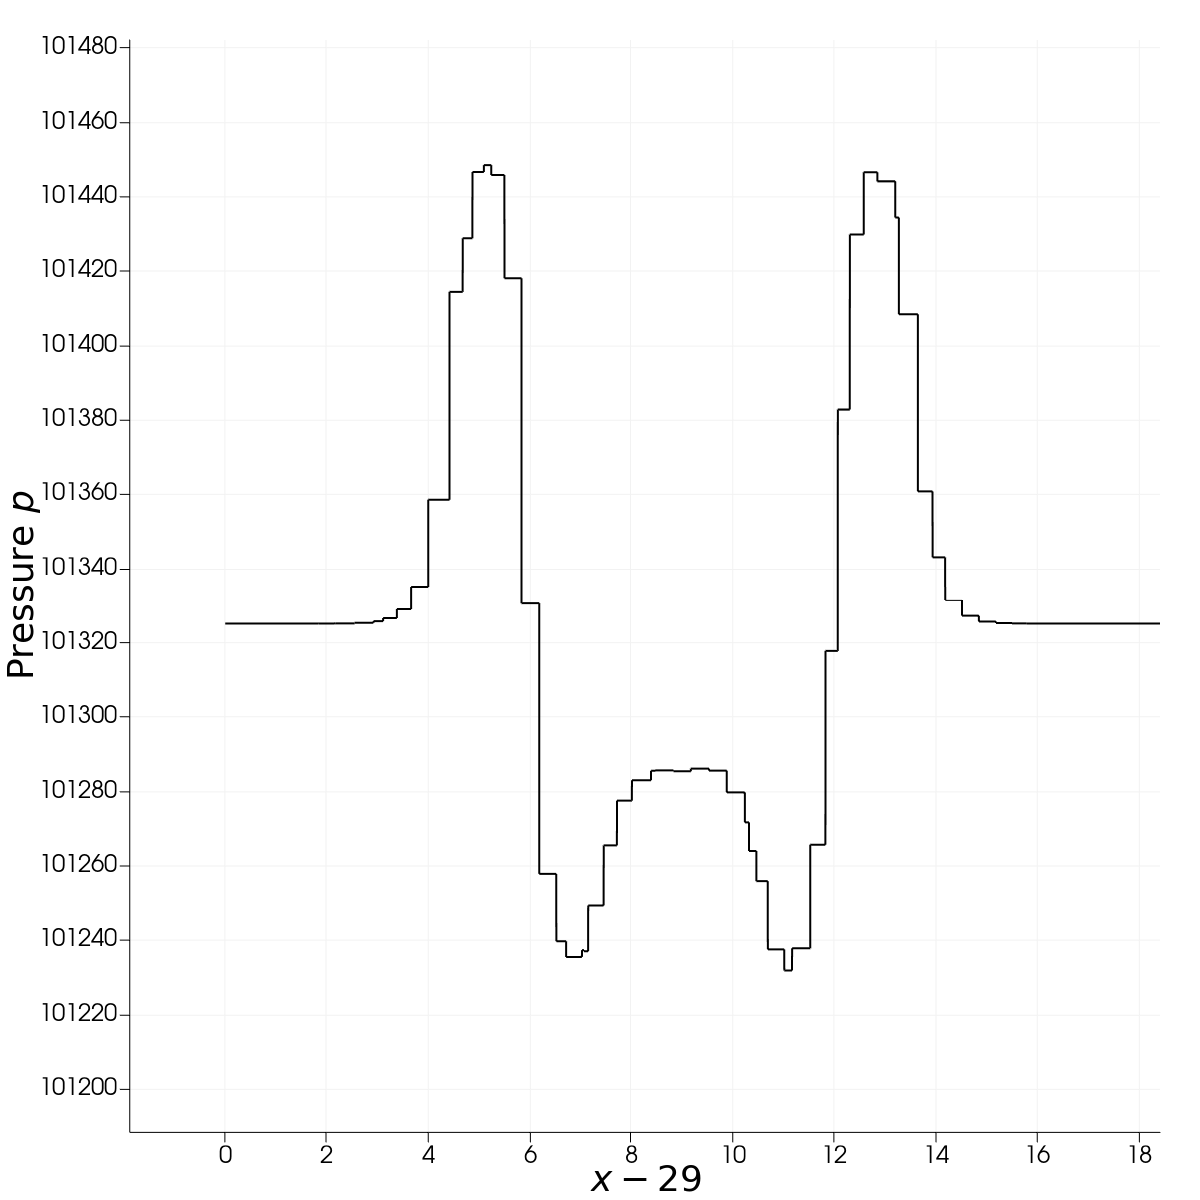
\includegraphics[width=0.85\textwidth]{ellipseP001.png}
\caption{Pressure on the $x$-axis at time $t = 0.01$.}
\label{fig:ellipse-P001}
\end{figure}










































\begin{appendices}
\chapter{Tensor calculus} \label{ch:appendix-tensors}

A matrix is more than just a 2D array of numbers: a matrix represents
a linear transformation between vector spaces.
If we choose different basis for the vector spaces, then the entries of the matrix
must change accordingly, so that the underlying transformation remains
the same: in some sense, the two changes must cancel out.

Likewise, a tensor is more than just an $n$-dimensional array of numbers:
a tensor represents an element of the tensorial product of two or more
vector spaces with respect to a (tensorial) basis.
Once again, the key difference is that the entries of a tensor must
change in a well-defined way every time a different basis is chosen
for the vector spaces. This is why it is quite common in physics and other sciences
to define tensors as \emph{anything that transforms like a tensor},
without getting into the details of how the tensor product is really defined
or how tensors could be introduced in a coordinate-free way.

It should be clear already that the same word, \emph{tensor},
has two slightly different meanings: a tensor can be the element
of the tensor product of two or more vector spaces (i.e.\ an intrinsic object),
but also its representation with respect to a fixed tensorial basis
(i.e.\ an array of real numbers).
As a rule of thumb, the first definition is better suited for proofs,
whereas the second one is better suited for calculations.
In the following, we will switch back and forth between the two
definitions; in Chapter 2, however, the word \emph{tensor} always has
the latter meaning.
Sometimes, a \emph{tensor field} (that is, a map which assigns
a tensor to each point of a domain) will also be referred to as a tensor.
This is why we speak of \emph{stress tensor} in a continuum instead of
\emph{stress tensor field}, for example.

%The rest of the appendix is organized as follows.
%First, the tensor product of two vector spaces is defined in the case in
%which a basis is fixed on both spaces (a coordinate-free definition
%would be too abstract for our purposes).
%Second, the standard notation of tensorial calculus is introduced,
%including the Einstein summation convention.
%Lastly, we explain how the entries of a tensor change when
%a different basis is chosen for the vector spaces on which the
%tensor is defined.

\subsection*{Definition of tensor product}

Let $U,V$ be finite dimensional real vector spaces with basis
$\{\vec{u}_i\}_{i = 1 \ldots m}$ and $\{\vec{v}_j\}_{j = 1 \ldots n}$, respectively.
We define the vectorial space $U \otimes V$ as the space of formal
linear combinations of the elements $\vec{u}_i \otimes \vec{v}_j$,
which by definition will then form a basis of $U \otimes V$.
Moreover, we endow the space $U \otimes V$ with a map
\[
\varphi \colon U \times V \to U \otimes V
\qquad
\varphi(\vec{u}_i,\vec{v}_j) = \vec{u}_i \otimes \vec{v}_j
\]
extended by bilinearity on the whole domain,
which allows us to give meaning to the expression $\vec{u} \otimes \vec{v}$
for all $\vec{u}$ in $U$ and all $\vec{v}$ in $V$: $\vec{u} \otimes \vec{v}$
is simply $\varphi(\vec{u},\vec{v})$.

It is a universal property of the tensor product that every bilinear map
$h \colon U \times V \to \R$ can be factored uniquely as the composition of
$\varphi$ and a linear map $\tilde{h} \colon U \otimes V \to \R$.
The vector space $U \otimes V$ has dimension $mn$, so it is trivially isomorphic
to the space $V \otimes U$. However, by using the coordinate-free definition
of tensor product, it is possible to prove that this isomorphism is canonical,
i.e.\ it can be defined without fixing any base on $U$ and $V$.
Likewise, it is also possible to prove that the space $(U \otimes V) \otimes W$
is canonically isomorphic to $U \otimes (V \otimes W)$: the tensor
product is, up to isomorphisms, a commutative and associative operation
between vector spaces.

\subsection*{Type $(r,s)$ tensors}

Let $V^*$ be the dual space of $V$, and let $\{\vec{v}^j\}$ be the dual basis
on $V^*$ (that is, the basis of functionals such that
$\vec{v}^j(\vec{v}_k) = \delta_{jk}$).
Commutativity and associativity of the tensor product together imply that,
in the definition of the following space, there is no loss of generality
given by the order of the factors involved:
\[
T^r_s(V) = \underbrace{V \otimes \dots \otimes V}_{\text{$r$ times}}
\otimes
\underbrace{V^* \otimes \dots \otimes V^*}_{\text{$s$ times}}.
\]
An element of the space $T_s^r(V)$ is known as \emph{type $(r,s)$ tensor}
on the space $V$. By definition, a type $(0,0)$ tensor is a scalar,
a type $(1,0)$ tensor is a vector, and a type $(0,1)$ tensor is a covector.
Tensor fields in differential geometry, continuum mechanics,
etc, are usually type $(r,s)$ tensors on the tangent space of some manifold.

Let $\tns{T}$ be an element of the space $T_s^r(V)$.
The representation of the tensor $\tns{T}$ with respect to the
tensorial basis
\[
\vec{v}_{i_1} \otimes \dots \otimes \vec{v}_{i_r}
\otimes
\vec{v}^{j_1} \otimes \dots \otimes \vec{v}^{j_s}
\]
is given by the $n^{r+s}$ scalars $\tns{T}^{i_1 \dots i_r}_{j_1 \dots j_s}$
such that
\[
\tns{T} = \sum_{i_1=1}^n \dots \sum_{i_r=1}^n \;\;
\sum_{j_1=1}^n \dots \sum_{j_s=1}^n \;\;
\tns{T}^{i_1 \dots i_r}_{j_1 \dots j_s} \;\;
\vec{v}_{i_1} \otimes \dots \otimes \vec{v}_{i_r}
\otimes
\vec{v}^{j_1} \otimes \dots \otimes \vec{v}^{j_s}.
\]
The indices $i_1, \dots, i_r$ of the coefficients are known as
\emph{contravariant indices}, and are always written as superscripts,
whereas the indices $j_1, \dots, j_s$ are known as \emph{covariant indices},
and are always written as subscripts.
Hence, the type of a tensor can be deduced by counting the number
of superscripts and subscripts. Sometimes, uppercase multi-indices are
used to group indices and simplify notation:
\[
\tns{T} = \sum_{I \in [1,n]^r} \; \sum_{J \in [1,n]^s}
\tns{T}^I_J \; \vec{v}_I \otimes \vec{v}^J.
\]

\subsection*{Contraction of tensors}

The most important operation involving tensors is \emph{contraction}.
Let $\tns{T}$ be a tensor of type $(r,s)$ with $r,s \geq 1$, let
$i$ be one of its contravariant indices and let $j$ be one of its
covariant indices.
The contraction of $\tns{T}$ with respect to $i$ and $j$ is the
type $(r-1,s-1)$ tensor obtained by substituting $i$ and $j$ with
a common index (say, $k$) and then summing over it:
\begin{equation} \label{eq:def-contraction}
\tns{T}^{\dots i \dots}_{\dots j \dots}
\quad \longrightarrow \quad
\tns{T}^{\dots k \dots}_{\dots k \dots}
\quad \longrightarrow \quad
\sum_{k=1}^n \tns{T}^{\dots k \dots}_{\dots k \dots}
\end{equation}
The fact that contraction produces a tensor and not just any multidimensional
array of numbers is a remarkable fact. The most elegant way to prove
this property would be to define contraction in an intrinsic way, using the
natural pairing of a vector space with its dual, and then to show
that this abstract definition corresponds to \eqref{eq:def-contraction}
as soon as a basis is fixed on $V$. For the sake of brevity, however,
we shall skip this proof.

Whenever two tensors of type $(p,q)$ and $(r,s)$ are written
one next to the other with no indices in common, they can be thought
of as a single tensor of type $(p+r,q+s)$, whose elements are
the product of the elements of the two tensors with corresponding indices:
\[
\tns{A} \in T^p_q(V), \; \tns{B} \in T^r_s(V) \qquad
(\tns{AB})^{IK}_{JL} = \tns{A}^I_J \tns{B}^K_L.
\]
This operation is known as \emph{outer product}, and sometimes
is written explicitely using the tensor product symbol $\otimes$.
If one contravariant index of a tensor is labeled with the same letter
as one covariant index of the other tensor, however,
contraction is implied and a tensor of type $(p+r-1,q+s-1)$ is produced.
This is known as \emph{Einstein summation convention}, and allows us
to drastically reduce the number of summation symbols required
to write most tensorial identities. For example, the contraction
$\sum_{j=1}^n \tns{A}^i_j \tns{v}^j$
can be written more succintly as $\tns{A}^i_j \tns{v}^j$.
This contraction of a type $(1,1)$ tensor with a type $(1,0)$ tensor
(which, by definition, is just a vector) is particularly meaningful:
the result is again a type $(1,0)$ tensor, so we have shown that a type
$(1,1)$ tensor can be naturally though of as a linear application from $V$
to itself. Following this idea, it is possible to prove that the space
$T^1_1(V)$ is canonically isomorphic to the space of linear operators on $V$,
and that, once a basis is fixed on $V$, a type $(1,1)$ tensor is essentially
a matrix. It is in this sense that contravariant indices and covariant indices
of tensors can be understood as generalizations of column indices
and row indices of matrices, respectively.

\subsection*{Change of basis formula}

Let $\{\tilde{\vec{v}}_j\}_{j = 1,\dots,n}$ be another basis on $V$,
and let $\mat{M}$ be the change of basis matrix from $\{\vec{v}_j\}$
to $\{\tilde{\vec{v}}_j\}$, i.e.\ the matrix such that
\[
\tilde{\vec{v}}_j = \sum_{k=1}^n \mat{M}^k_j \vec{v}_k.
\]
Let $\tns{T}^{i_1 \dots i_r}_{j_1 \dots j_s}$ be the representation
of a type $(r,s)$ tensor $\tns{T}$ with respect to the basis $\{\vec{v}_j\}$.
Then, it can be proved that the representation of the same tensor $\tns{T}$
with respect to the new basis $\{\tilde{\vec{v}}_j\}$ is given by
\begin{equation} \label{eq:tensor-change-of-basis}
\tilde{\tns{T}}^{k_1 \dots k_r}_{\ell_1 \dots \ell_s}
= \tns{T}^{i_1 \dots i_r}_{j_1 \dots j_s} \,
(\tns{M}^{-1})_{i_1}^{k_1} \dots (\tns{M}^{-1})_{i_r}^{k_r} \,
\tns{M}^{j_1}_{\ell_1} \dots \, \tns{M}^{j_s}_{\ell_s}.
\end{equation}
The converse is also true: if a multidimensional array of numbers
satisfies this change of basis formula, then the array is a tensor
(that is, there exists an \emph{intrinsic} tensor in $T^r_s(V)$ whose
representation is given by the array). This gives us another way of proving
that contraction, as defined above, is a well-defined operation.
On the other hand, it's easy to see that contraction with respect
to a pair of contravariant indices or a pair of covariant indices would be
ill-defined, because the result wouldn't transform like a type $(r-2,s)$
tensor or type $(r,s-2)$ tensor, respectively.

\subsection*{Metric tensor}

The contraction $\tns{A}_{ij} \tns{v}^i \tns{w}^j$, which produces
a real number, is also of great importance, because it shows
that the space $T^0_2(V)$ is canonically isomorphic to
the space of bilinear forms on $V$. Working with coordinates, this means
that a type $(0,2)$ tensor like $\tns{A}_{ij}$ is just a Gram matrix.

Let $\langle \cdot, \cdot \rangle$ be a positive-definite scalar product
on $V$, and let $\mat{G}$ be its Gram matrix with respect to the same
basis on $V$ that was used to define the tensorial basis on the spaces $T^r_s(V)$.
Let $\tns{g}_{ij}$ be the type $(0,2)$ tensor associated to $\mat{G}$.
Then, $\tns{g}_{ij}$ is known as \emph{metric tensor}, and $\tns{g}_{ij}$
can be used to calculate the scalar product between any two vectors
$\vec{v}$ and~$\vec{w}$:
\[
\langle \vec{v}, \vec{w} \rangle = \tns{g}_{ij} \tns{v}^i \tns{w}^j.
\]
If the basis on $V$ is orthonormal with respect to the chosen scalar
product, then the metric tensor is given by Knonecker's delta:
$\tns{g}_{ij} = \delta_{ij}$. The metric tensor can also be used
to \emph{lower} an index of a tensor. Let $\tns{A}^{Ik}_J$ be
any type $(r+1,s)$ tensor with at least one contravariant index,
in this case~$k$. Then, if we contract $\tns{A}$ with $\tns{g}$ we
say that we are \emph{lowering} the index $k$, as a new tensor $\tns{B}$
of type $(r,s+1)$ is produced:
\[
\tns{B}^I_{J \ell} = \tns{A}^{Ik}_J \tns{g}_{k \ell}.
\]
The name of this operation comes from the fact that, in the common case in which
the metric tensor is equal to Knonecker's delta, the result is obtained by
literally lowering the index $k$. However, in the general case, the
presence of the metric tensor is required to ensure that the result
satisfies the change of basis formula \eqref{eq:tensor-change-of-basis}
(in other words, that the operation is intrinsic).

The metric tensor $\tns{g}_{ij}$ has an inverse, namely $\tns{g}^{jk}$,
that satisfies the identity $\tns{g}_{ij} \tns{g}^{jk} = \delta_{ik}$
and that is given by the inverse of the Gram matrix $\mat{G}$
(this is always possible, because $\mat{G}$ is positive definite).
The inverse of the metric tensor can be used to \emph{raise} indices
in the same way that the metric tensor can be used to lower indices.

We've seen that contraction of a tensor is only well-defined when
a contravariant index is paired with a covariant one.
However, by lowering or raising indices appropriately first, contraction
can also be done with respect to a pair of contravariant indices
or covariant ones: the presence of the metric tensor or its inverse
makes the change of basis formula hold this time.

\subsection*{Differential operators}

Let $\tns{T}^I_J(\vec{x})$ be a type $(r,s)$ tensor field on an open subset
of $\R^n$ (the more general case of a differential manifold
is not needed for our purposes), let $V = \R^n$ and
let $\{\vec{e}_k\}_{k = 1,\dots,n}$ be the canonical basis of $\R^n$.
Just like with scalar and vector fields, the $k$-th partial derivative
$\partial_k \tns{T}^I_J$ of the tensor field $\tns{T}^I_J$ in $\vec{x}$
can be defined as the limit
\[
\partial_k \tns{T}^I_J(\vec{x})
= \lim_{h \to 0} \frac{
	\tns{T}^I_J(\vec{x}+h\vec{e}_k) - \tns{T}^I_J(\vec{x})
	}{h},
\]
provided that such a limit exists (i.e.\ the tensor field is sufficiently
regular). Partial derivatives are linear operators and satisfy the product
rule and the chain rule. The fact that $k$ is written as a subscript
is not by chance: it can be proved that $\partial_k \tns{T}^I_J(\vec{x})$
is a type $(r,s+1)$ tensor field, called \emph{total derivative}
of $\tns{T}^I_J(\vec{x})$. The \emph{gradient} of a tensor field is
defined by raising the covariant index $k$ using the metric tensor:
\[
\nabla \tns{T}^I_J(\vec{x}) = \partial^k \tns{T}^I_J(\vec{x}).
\]
In this way, we generalize to tensors the fact that the gradient of
a scalar field is a column vector, whereas the total derivative
(or \emph{total differential}) of a scalar field is a row vector.

The divergence of a tensor field can be defined by pointwise
contraction of a contravariant index of the tensor field with
the covariant index of $\partial_k$. For example, given a vector
field $\vec{v}^j(\vec{x})$, its divergence $\diver(\vec{v})$
is the scalar field $\partial_k \vec{v}^k(\vec{x})$.
When the tensor field has more than one contravariant index, it is good
practice to add a subscript to $\diver(\cdot)$ for additional clarity:
compare $\diver_i(\tns{T}^{ij})$ with $\diver_j(\tns{T}^{ij})$.

% divergence theorem with dot product?



















\lstset{inputpath = ../MATLAB}

\chapter{Source code}  \label{ch:appendix-source-code}

\end{appendices}

\printbibliography[heading=bibintoc]

\end{document}


























